
\documentclass[12pt]{article}

\title{Semiparametric SDF Estimators \\ for Pooled, Non-Traded Cash Flows}

\author{
	Christian Tausch  \\
	AssetMetrix GmbH  \\
	Theresienh\"{o}he 13, D-80339 Munich \\
	christian.tausch@quant-unit.com \\
	\and 
	Alexander Bohnert  \\
	Munich University of Applied Sciences \\
	Am Stadtpark 20, D-81243 Munich \\
	alexander.bohnert@hm.edu \\
}

\date{\today}



% Packages
\usepackage{amssymb}
\usepackage{amsmath}
\usepackage{natbib}
\usepackage{graphics}
% use smaller margins
\usepackage[margin=1.1in]{geometry} % 1.25in
\usepackage[margin=1.1cm]{caption}
% use double spacing
\usepackage{setspace}
\usepackage{amsthm}
\usepackage{url}
\usepackage[outdir=./]{epstopdf}
\usepackage{booktabs}
\usepackage{float}
\usepackage{standalone}
\usepackage{xcolor}
\usepackage{tabularx}


\newtheorem{assume}{Assumption}
\newtheorem{lemma}{Lemma}
\newtheorem{proposition}{Proposition}
\newtheorem{corollary}{Corollary}
\newtheorem{remark}{Remark}
\newtheorem{definition}{Definition}
\newtheorem{example}{Example}
\newtheorem{theorem}{Theorem}


% logo
\usepackage{fancyhdr}
\usepackage{graphicx }



\begin{document}
	
\maketitle


\section*{Keywords}
Stochastic Discount Factor,
Semiparametric Estimation,
Spatial Dependence,
Generalized Method of Moments (GMM),
Private Equity,
Illiquid Assets


\section*{Acknowledgements}
We thank Nicolas D\"{u}tsch, Philipp Abel, and Kai Urban for valuable feedback and helpful comments that greatly improved the paper.
%Further, we want to thank Jingzhi Huang, the editor, and two anonymous referees for their inspiring suggestions that helped to significantly improve the depth and robustness of our paper.


\section*{Declaration of interest}
The authors report no conflict of interest. 
The authors alone are responsible for the content and writing of the paper.


\newpage
%\doublespacing

\begin{center} 
	\section*{Semiparametric SDF Estimators \\ for Pooled, Non-Traded Cash Flows}
\end{center}



\abstract{
	This paper analyzes stochastic discount factor estimation methodologies suited for pooled, non-traded cash flow streams such as the fund-level cash flows of private equity funds.
	The asymptotic inference framework for our semiparametric nonlinear least squares estimator draws on a spatial notion, i.e., the idea that the economic distance between distinct private equity funds can be measured.
	The empirical and Monte Carlo simulation results indicate (i) that our method can improve the popular Generalized Method of Moments approach of \cite{DLP12}, but (ii) that estimator variance for typical data sizes is still high.
	Thus, we conjecture that traditional semiparametric extremum estimators like the one described by us shall be exclusively used for single-factor models until considerably more vintage year information for private equity funds is available.
}


%% main text
\section{Introduction}

Private equity has outgrown its niche, sitting today on more than \$9 trillion in assets under management, yet rigorous asset-pricing tools have not kept pace with this ascent.
The empirical analysis and risk assessment of private equity and other non-traded cash flows remain fundamentally challenging due to the absence of market-based valuations and the inherent frictions of private markets (i.e., under incomplete information). 
Unlike public assets with trusted and tradeable valuations (in liquid secondary markets), private equity investments generate irregular, infrequently observed cash flows for which standard return-based asset pricing techniques are unsuitable.

We address this gap by proposing a semiparametric stochastic discount factor (SDF) estimator tailored to fund-level cash flows that refines the SDF estimators of \cite{DLP12} and \cite{KN16}.
Our nonlinear least squares estimator stems from the class of Least-Mean-Distance (LMD) estimators, which are easier to handle than traditional Generalized Method of Moments (GMM) approaches \citep{PP97}.
Our LMD estimator arguably both simplifies and generalizes the GMM methodology of \cite{DLP12}, where we provide the asymptotic inference framework that was missing in the original paper.
The asymptotic inference formulations rely on the concept of spatial (near-epoch) dependence between funds as proposed by \cite{KN16}.
In this context, it is paramount to quantify the economic distance between funds by a measure like absolute vintage year difference or cash flow overlap\footnote{However, this economic inter-fund \emph{distance} refers \textbf{not} to the term Least-Mean-\emph{Distance} estimator.}.`

For fund-level cash flow data of private equity funds, we document an asymptotic bias term for cash-flow-based SDF estimators like \cite{DLP12} and \cite{KN16} that persists also in large samples.
The bias term arises due to the pooled nature of fund-level cash flows and more specifically because of the different starting dates of the underlying deals (in the fund investment period).
Our estimator offers simple averaging over multiple discounting dates as one option to control (but not eliminate) the bias term.

In the empirical application of our new estimator, we test simple linear and exponentially affine SDF models that can draw on the five return factors associated with the $q^5$ investment factor model recently proposed by \cite{HXZ20}.
Based on a Spatial Heteroskedasticity and Autocorrelation Consistent (SHAC) covariance matrix estimator, we calculate asymptotic standard errors for the model coefficients.
Moreover, we assess the small-sample variance of coefficient estimates and the out-of-sample performance of the different SDF models by $hv$-block cross-validation, which accounts for the inter-vintage-year dependence of private equity funds \citep{R00}.
We test one- and two-factor models for the most prominent private capital fund types Private Equity (PE) and Venture Capital (VC).
The empirical two-factor model results are rather disappointing; not more than the single-market-factor model results seem reasonable given the high estimator variance.

The paper is structured as follows. 
% Section \ref{sec:literature} reviews the related literature.
Section \ref{sec:spatial_sdf_methodology} introduces our semiparametric LMD estimator and its corresponding asymptotic inference framework.
Section \ref{sec:empirical_application} applies the method to estimate $q^5$-investment-factor SDFs for various private equity fund types using simulated and real-world cash flows.
Section \ref{sec:spatial_sdf_conclusion} concludes.


\iffalse

\section{Literature}
\label{sec:literature}

For private equity funds, performance evaluation under the SDF framework is currently an active research topic \citep{DLP12,FNP12,B14,B16a,B16b,KN16,ACGP18,GSW19}.
Previously, SDF performance evaluation was already applied for public stock markets by, e.g., \cite{FFJT02} and for hedge fund returns by \cite{LXZ16}.

In our literature review, we focus on the most relevant parametric and semiparametric estimation methods for private capital fund cash flows.


\subsection{Parametric approach}

\cite{ACGP18} contribute a parametric approach using Bayesian Markov Chain Monte Carlo methods to estimate latent return factors from present value ratios.
\cite{ACGP18} use fund-level data provided by Preqin to estimate a "PE return index based on historical fund cash flows."
As Data Generating Process (DGP), they assume a log-linear factor model for each fund distribution
\begin{equation}
	\label{eq:data_generating_process}
	D_T = C_t \prod_{\tau=t+1}^{T} g_{\tau}
\end{equation}
where $D_T$ is a given fund distribution and $C_t$ a contribution with $t<T$.
The return dynamics $\ln (g_t) = \ln (g_t^M) + \epsilon_t$ where $g_t^M$ is the market component of the fund return and $\epsilon_t$ its idiosyncratic part that is normal and i.i.d.
The state space dynamics of the filtering problem describe the factor model structure of $g$ as
\[
g_t^M = \alpha + r_t^{\mathrm{free}} + \beta^{\top} F_t + f_t^{\mathrm{PE}}
\]
where $\alpha$ is the average excess return, $r_t^{\mathrm{free}}$ is the risk-free rate, $F_t$ is a vector of public market (long-short) factor returns, $\beta$ the corresponding factor loadings, and $f_t^{\mathrm{PE}}$ is "an asset-class-specific latent factor with mean zero that is orthogonal to the traded factors, $F_t$."
They assume each fund holds $N$ investments $i=1,2,\dots,N$; $t_i$ notes the investment date of the first deal and $T_i$ is the corresponding exit date.
For each fund, they then postulate the following Present Value Ratio ($PVR$) to hold
\begin{equation}
	\label{eq:pvr_ang_2018}
	PVR = \ln \left(\frac{PV_D}{PV_C}\right) \cong \ln (u) \qquad \mathrm{where} \quad \ln (u) \sim N \left( - 0.5 \sigma^2, \sigma^2 \right)
\end{equation}
with present value of distributions
\[
PV_D = \sum_{i=1}^N \frac{D_{T_i}}{g_{t_1} \dots g_{T_i}}
\]
and present value of contributions
\[
PV_C = \sum_{i=1}^N \frac{C_{i}}{g_{t_1} \dots g_{T_i}} U_{t_i, T_i}
\]
where $U_{t_i, T_j}$ contains the idiosyncratic terms
\[
U_{t_i, T_j}^i = \exp \left( \epsilon_{t_i + 1} + \dots + \epsilon_{T_i} \right)
\]
Here, the approximation ($\cong$) of the PVR by $\ln (u)$ relies on a lognormal central limit theorem (CLT) obtained from the textbook of \cite{BT13}.
For this CLT to hold, they need the two \textbf{regularity conditions} that there is no dominantly (i) large or (ii) long investment as $N$ goes to infinity.
They estimate all relevant model parameters, i.e., $\alpha,\beta$ and the latent residual return time-series $f^{\mathrm{PE}}$, by a Bayesian Markov Chain Monte Carlo method that minimizes "one large error term per fund in the estimation process".
Thus \cite{ACGP18} provide the first SDF estimation method in the literature that not only estimates the public market factors but additionally an \textbf{asset-class-specific latent factor}.
Because of the high dimensionality of $f^{\mathrm{PE}}$ (i.e., a return time-series), they need to employ an estimation method like Gibbs sampling that can handle more parameters to estimate than actual data points.
Inspired by these ``latent factors", \cite{TP24} propose a machine-learning approach to estimate the error-term time series of public factor models for private capital funds.

\subsection{Semiparametric approaches}

Semiparametric approaches omit (i) parametric specifications for the idiosyncratic error term and (ii) often also formulations of the concrete Data Generating Process (DGP).

\cite{DLP12} develop the first SDF estimator tailored for typical PE fund-level cash flows.
Their goal is to estimate a linear factor model that minimizes the squared $DNCF$ of PEFs.
Generically, they solve the following minimization problem
\begin{equation}
	\label{eq:dlp12_minimization}
	\theta^{\mathrm{SDF}} = 
	\arg \min_{\theta^{\mathrm{SDF}}} \sum_{i=1}^N 
	\left[ 
	\sum_{t=1}^{T_i}
	\left(
	\frac{D_{it} - C_{it}}{\Psi_{t}^{-1}}
	\right)
	\right]^2
\end{equation}
where $N$ is the number of PEF portfolios in the dataset.
$\theta^{\mathrm{SDF}}=(\alpha, \beta)$ are the coefficients of a linear factor model SDF with $\Psi_t=(\prod_{\tau=0}^t R_{\tau})^{-1}$ where $R_{\tau}$ follows a \textbf{linear return factor model}
\begin{equation}
	R_{\tau}=1+\alpha_{\tau}+\beta^{\top}F_{\tau}+\epsilon_{\tau}
\end{equation}
where the risk-free rate is the first element of the vector $F_{\tau}$.
Plugging these terms into Equation \ref{eq:dlp12_minimization} yields
\[
\left( \alpha, \beta \right) 
= 
\arg \min_{\alpha, \beta} 
\sum_{i=1}^N 
\left( 
\sum_{t=1}^{T_i}
\frac{D_{i,t} - C_{i,t}}{\prod_{\tau=0}^t (1 + \alpha_{\tau}+\beta^{\top}F_{\tau}+\epsilon_{\tau}) } 
\right)^2
\]
which constitutes a nonlinear least squares optimization problem.
However, \cite{DLP12} \textbf{interpret their approach as Generalized Method of Moments (GMM) estimator} with $N$ moment conditions and identity weighting matrix where asymptotically the number of underlying investments per portfolio $i$ tends to infinity.
In our view, this cross-sectional GMM interpretation is both unnecessarily (i) complex and (ii) unrealistic.
Especially, their GMM derivation (in the internet appendix) takes as starting point a DGP similar to Equation \ref{eq:data_generating_process} but does not show why their nontraditional GMM interpretation is favorable to traditional (and simpler) non-linear least squares as defined, e.g., by \cite{PP97}.
Instead of using individual funds, they form $N$ \textbf{vintage year portfolios} where they pool all fund cash flows from a given vintage "to lower the effect of idiosyncratic shocks," similar to \cite{FNP12}.
To obtain standard errors for their coefficient estimates, the authors rely on cross-sectional bootstrapping \textbf{instead of providing} an asymptotic inference formula.
Empirically, the paper draws on the problematic Thomson Venture Economics (TVE) fund-level dataset that exhibits some now well-known data errors as discussed by \cite{HJK14}.
For VC, they estimate a one-factor model with a market beta factor of 2.73 and an annualized negative alpha of -12.3\%. For BO, one-factor model coefficients are 1.31 for the market factor, and the annualized alpha is again negative with -4.8\%.
These highly negative alpha terms can be at least partially attributed to the aforementioned data errors in the TVE dataset.
However, surprisingly from a methodological viewpoint, both alpha terms must be considered insignificantly different from zero due to high bootstrap standard errors.
In summary, we still consider the \cite{DLP12} paper a seminal contribution to the PE literature as it proposes the first semiparametric SDF estimator for typical PEF (fund-level) datasets.  


\cite{KN16} introduce the Generalized Public Market Equivalent (GPME) framework, which is a new SDF-based performance evaluation methodology for PE fund-level cash flows.
The general idea is to first estimate a given SDF just on a public market dataset and then, in the second step, evaluate PEF cash flows by a traditional NPV approach
\[
GPME = \sum_t \Psi_t^{\mathrm{public}} CF_t^{\mathrm{PEF}}
\]
where $\Psi_t^{\mathrm{public}}$ is a generic SDF estimated on public data and $CF_t^{\mathrm{PEF}}$ are all cash flows of a (liquidated) PEF.
Here, GPME is simply our DNCF from Equation \ref{eq:net_present_value}.
However, their paper also offers one new and important methodical insight for SDF estimation using PE cash flow data.
They are the first to realize that for asymptotic statistical inference, a \textbf{spatial heteroskedasticity and autocorrelation consistent (SHAC)}\footnote{A SHAC estimator will be later applied and defined by Equation \ref{eq:hac}.} covariance matrix estimator that incorporates the economic distance between PE fund pairs proves very useful.
To estimate their exponentially affine SDF, they apply a time-series Generalized Method of Moments (GMM) approach where they, for simplicity, assume an identity weighting matrix.
This corresponds to a very similar minimization problem as the one from Equation \ref{eq:dlp12_minimization}, which is used by \cite{DLP12}. 
They form public replication portfolios that mimic PEF contributions and distributions patterns and use these synthetic cash flows for SDF estimation. 
Interestingly, they claim that an exponentially affine SDF is especially suited for "irregularly spaced, skewed, and endogenously timed payoffs" of VC investments.
Moreover, they state: "With irregularly spaced and skewed VC cash flow data, \textbf{linear factor models are not readily applicable} without strong distributional assumptions."
Empirically, the authors calculate their GPME metric for VC funds from the Preqin fund-level dataset and start-ups from Sand Hill Econometrics' deal-level data.
Unfortunately, they relinquish to also test a linear factor model as an alternative to their exponential affine SDF to underpin their strong allegation about the correct SDF choice.
It is also not clear why they cannot use a public SDF that has been estimated on a traditional public stock return (not cash flow) dataset (comparable to the \cite{GSW19} approach, which is discussed in the next paragraph).
From this perspective, their non-traditional GMM estimator and the construction of the public benchmark portfolio cash flows seem unnecessarily complicated and artificial.

In a more recent paper \cite{KN22} extend their GPME methodology to obtain risk-adjusted benchmarks for single PE funds.
\cite{NSS22} adapt the GPME method to estimate their so-called Credit Market Equivalent which relies on an SDF that prices the bonds issued by buyout-held companies.
Interestingly, \cite{NSS22} find that public credit market factors can better price PE cash flows than the traditional public stock market factors.
Similarly, \cite{GJ21} test the GPME approach using a CAPM SDF and a "Discount Rate News" SDF.
Although we think pricing PE cash flows instead of public market cash flows is the more natural approach (as \cite{GJ21} and \cite{NSS22} did), \cite{KN16,KN22} still mark highly significant contributions to the PE-related SDF literature.

The unpublished working paper of \cite{GSW19} evaluates PE fund-level cash flows by means of asset pricing tests for ``off-the-shelf" SDFs.
They examine SDFs that shall be presumably better aligned with typical PE investor preferences than traditional factor models like \cite{FF15}.
Specifically, they test two leading consumption-based asset pricing models: the long-run risk model of \cite{BY04} and the external habit formation model of \cite{CC99} among other simpler SDF alternatives.
Notably, in the first place, the authors take SDF parameters from the existing literature rather than estimating their own SDF coefficients.
This is comparable to the \cite{KN16} generalized PME framework, which also does not uses any PE cash flows for SDF estimation.
Their SDF can thus be considered as universal SDFs that can price all cash flows in a given economy (not just PE cash flows specifically).
Just in their additional results section \cite{GSW19} ``are trying to 'fine-tune' the off-the-shelf SDFs to reduce the benchmark pricing errors".
Empirically, they obtain unrealistically large negative risk-free rate parameters when fitting SDFs to fund cash flows from the Burgiss database.
Most interestingly, they claim to ``show that cash flow NPV-based measures of performance for long-duration investment vehicles like PE funds are biased relative to per-period abnormal return estimates."
In other words, they criticize asset pricing tests that are based on a general NPV-equal-to-zero condition (cf.\ Equation \ref{eq:basic_pricing_relation}).
Their derived bias term is non-zero if there exits any auto-correlation in the time-series of (unobserved) pricing errors $e_t = \Psi_t R_t - 1$ were $\Psi_t$ is a SDF and $R_t$ is the latent periodic PE return.
Here they assume a data generating process similar to Equation \ref{eq:data_generating_process}, which is used by \cite{ACGP18}.
\textcolor{red}{
	To better understand their ``compounding error" \textbf{small-sample bias}, it is important to mention that in small samples, we may measure a nonzero autocorrelation for some error terms even if this effect vanishes asymptotically and the true expected autocorrelation is zero.
	}
So, we generally agree that asset pricing tests for PE cash flow datasets are always weaker than standard time-series asset pricing tests that could draw on the latent true return time-series of PE returns.
Moreover, their idea to \textbf{price the difference between PE cash flows and a suitable public replication strategy} instead of just PE cash flows (as a resolution of their bias issue) is picked up by the quadratic hedging strategies derived by \cite{T19}.

\fi


\section{Methodology}
\label{sec:spatial_sdf_methodology}

Our general SDF estimation framework is similar to that of \cite{DLP12} and \cite{KN16}; 
the subtle but important differences are discussed in Section \ref{sec:comparison_to_similar_estimators}.

In a nutshell, the \cite{DLP12} estimator determines the optimal alpha and beta parameters of a linear factor model by minimizing the net present value (NPV) of all $N$ fund cash flows.
\begin{equation}
	\min_{\alpha,\beta} = \sum_{i=1}^N \left[ {NPV}_i(\alpha,\beta) \right]^2
\end{equation}
with NPV for the $i$th fund
\[
{NPV}_i(\alpha,\beta) =
\sum_{t \in \left\{ t_{0,i}, t_{0,i} + 1, \dots \right\}}
\frac{\mathrm{CashFlow}_{t,i}}{
	\prod_{s=t_{0,i}}^{t}
	\left( 
	1 + r_{\mathrm{free}, s} + \alpha + \beta r_{\mathrm{market}, s}
	\right)
} 
\]
In this Methodology section, we will show:
\begin{enumerate}
	\item Why this estimator is usually asymptotically biased for pooled cash flows (Section \ref{sec:asset_pricing_pooled}).
	\item How to modify the estimator to be able to control the bias term (Sections \ref{sec:fundwise_lmd_estimator} and \ref{subsec:npv_vs_fv}).
	\item How we can estimate asymptotic standard errors for the parameters alpha and beta (Sections \ref{sec:asymptotic_framework} and \ref{sec:asymptotic_inference}).
\end{enumerate}


\subsection{Asset Pricing for Pooled Cash Flows}
\label{sec:asset_pricing_pooled}

Let fund $i=1,2,\dots,n$ be characterized by its net cash flows ${CF}_{t,i}$ (i.e., distributions minus contributions) and its net asset values ${NAV}_{t,i}$ with discrete time index $t=0,1,2,\dots,T$.
To increase the mathematical tractability of the problem, we assume a  deal-by-deal data generating processes (DGP) for $CF$ where each fund deal consists exactly of one investment and one divestment cash flow in combination with a simple return model for the multi-period deal returns.
This means the fund-level cash flow process $(CF_{i,t})_{t=0,1,...,T}$ is an aggregation of deal-level cash flow pairs consisting of one negative at deal inception and at least one positive cash flow later $CF_{t,i} = \sum_j^J {cf}_{j,i,t}$.
\begin{assume}
	\label{ass:deal_level_dgp}
	Deal-level data generation process: \\
	1. Each fund $i$ consists of $J$ underlying deals. \\
	2. Each deal is characterized by exactly one, negative investment cash flow, denoted by $\mathrm{Inv}_{i,j}$, which occurs at time $t_{i,j}^{\mathrm{Inv}} \in \{ 0,1,\dots, T-1 \}$. 
	It holds $\mathrm{Inv}_{i,j} < 0$. \\
	3. Each deal is characterized by a positive divestment cash flow stream, denoted by $(\mathrm{Div}_{i,j,k})_{k=1,\dots,K}$, which occur at after the investment cash flow $t_{i,j,k}^{\mathrm{Div}} > t_{i,j}^{\mathrm{Inv}}$ for all $k$.
	It holds $\mathrm{Div}_{i,j,k} > 0$. \\
	4. The cumulative fund cash flows are generated by summarizing over all deal-level cash flows, i.e., 
	$\sum_{t=0}^T {CF}_{i,t} = \sum_{j=1}^J \left( \mathrm{Inv}_{i,j} + \sum_k^K \mathrm{Div}_{i,j,k} \right)$ for all $i$.
\end{assume}

From asset pricing theory, we know that we can use a stochastic discount factor $\Psi_t$ to price each underlying deal
\begin{equation}
	\label{eq:deal_pricing}
	\mathbb{E} \left[ 
	\delta_{i,j}
	\left| \mathcal{F}_{t_{i,j}^{\mathrm{Inv}}} \right.
	\right] = 0
	\quad \forall \ i,j
\end{equation}
where we denote the deal-level pricing error by
\begin{equation}
	\delta_{i,j} :=
	\label{eq:deal_pricing_error}
	\mathrm{Inv}_{i,j} +
	\sum_k^K
	\frac{\Psi_{t_{i,j,k}^{\mathrm{Div}}}}{\Psi_{t_{i,j}^{\mathrm{Inv}}}}
	\mathrm{Div}_{i,j,k}
\end{equation}

For the pooled, fund-level cash flow stream, we assume that the true fund valuation $V_{i,\tau}$ is not observable for us
\begin{equation}
	\label{eq:fund_valuation}
	V_{i,\tau} :=
	\mathbb{E} \left[ 
	\sum_{t = \tau}^T
	\frac{\Psi_{t}}{\Psi_{\tau}}
	{CF}_{i,t}
	\left| \mathcal{F}_{\tau} \right.
	\right]
	\quad \forall \ \tau \geq \ \min_j \mathrm{Inv}_{i,j}
\end{equation}
to acknowledge the stale-pricing problem inherent to private capital fund net asset values (NAVs).
In other words, we only trust fund cash flows but not fund NAVs in private markets\footnote{In the empirical section, we empirically treat the most recent NAV as the final distribution cash flow for non-liquidated funds.}.

In this realistic setting, the absence of observable market valuations considerably contributes to the difficulty of our pricing problem.
However, also the existence of only pooled cash flows, instead of granular deal-by-deal cash flows, introduces issues for pricing approaches like \cite{DLP12} that discount to the fund inception date (see Equation \ref{eq:dlp12_minimization}).
In the following, we will demonstrate why we cannot easily price pooled fund-level cash flow streams without introducing \textbf{inevitable bias terms} (even for fund inception date $\tau = \min_j t_{i,j}^{\mathrm{Inv}}$).
Generally, all deal-level cash flows will produce the following ``bias term"
\begin{equation}
	\label{eq:deal_level_bias}
	\mathbb{E} \left[ 
	\frac{\Psi_{t_{i,j}^{\mathrm{Inv}}}}{\Psi_{\tau}}
	\delta_{i,j}
	\left| \mathcal{F}_{\tau} \right.
	\right]
	=
	\mathrm{Cov} \left[ \frac{\Psi_{t_{i,j}^{\mathrm{Inv}}}}{\Psi_{\tau}}, \ \delta_{i,j} \right]
	\quad \forall \ \tau < t_{i,j}^{\mathrm{Inv}}
\end{equation}
Only for the trivial case of Equation \ref{eq:deal_pricing}, where the investment date coincides with the discounting date $\tau =  t_{i,j}^{\mathrm{Inv}}$, the covariance term necessarily equals zero.

For the fund-level cash flows, we therefore introduce the following proposition.
\begin{proposition}
	\label{theo:pooled_bias}
	Price of a pooled cash flow stream at fund inception: \\
	\begin{equation}
		\label{eq:price_pooled_cash_flows}
		\mathbb{E} \left[ 
		\sum_{t = \tau}^T
		\frac{\Psi_{t}}{\Psi_{\tau}}
		{CF}_{i,t}
		\left| \mathcal{F}_{\tau} \right.
		\right]
		=
		\sum_{j=1}^J
		\mathrm{Cov} \left[ \frac{\Psi_{t_{i,j}^{\mathrm{Inv}}}}{\Psi_{\tau}}, \ \delta_{i,j} \right]
		\ \forall \ i
	\end{equation}
	with fund inception date $\tau = \ \min_j \mathrm{Inv}_{i,j}$.
\end{proposition}

We can simply proof the proposition as follows.
\begin{proof}
		We start with using Point 4 of Assumption \ref{ass:deal_level_dgp} which states that fund-level cash flows are the sum of deal-level cash flows.
		Further, we stipulate in the proposition that no deal-level cash flow occurs before $\tau$.
		Thus, the expected value of discounted fund-level cash flows needs to equal the expected value of discounted deal-level cash flows. 
		\begin{equation}
		\label{eq:price_pooled_cash_flows_proof_1}
		\mathbb{E} \left[ 
		\sum_{t = \tau}^T
		\frac{\Psi_{t}}{\Psi_{\tau}}
		{CF}_{i,t}
		\left| \mathcal{F}_{\tau} \right.
		\right]
		=
		\mathbb{E} \left[ 
		\sum_{j=1}^J
		\frac{\Psi_{t_{i,j}^{\mathrm{Inv}}}}{\Psi_{\tau}}
		\delta_{i,j}
		\left| \mathcal{F}_{\tau} \right.
		\right]
	\end{equation}
	Using Equation \ref{eq:deal_level_bias}, we can rewrite
	\begin{equation}
		\label{eq:price_pooled_cash_flows_proof_2}
		\mathbb{E} \left[ 
		\sum_{j=1}^J
		\frac{\Psi_{t_{i,j}^{\mathrm{Inv}}}}{\Psi_{\tau}}
		\delta_{i,j}
		\left| \mathcal{F}_{\tau} \right.
		\right]
		=
		\mathbb{E} \left[ 
		\sum_{j=1}^J
		\mathrm{Cov} \left[ \frac{\Psi_{t_{i,j}^{\mathrm{Inv}}}}{\Psi_{\tau}}, \ \delta_{i,j} \right]
		\left| \mathcal{F}_{\tau} \right.
		\right]
	\end{equation}
	Linearity of expectations then yields the result we want to proof.
		\begin{equation}
		\label{eq:price_pooled_cash_flows_proof_3}
		\mathbb{E} \left[ 
		\sum_{j=1}^J
		\mathrm{Cov} \left[ \frac{\Psi_{t_{i,j}^{\mathrm{Inv}}}}{\Psi_{\tau}}, \ \delta_{i,j} \right]
		\left| \mathcal{F}_{\tau} \right.
		\right]
		=
		\sum_{j=1}^J
		\mathrm{Cov} \left[ \frac{\Psi_{t_{i,j}^{\mathrm{Inv}}}}{\Psi_{\tau}}, \ \delta_{i,j} \right]
	\end{equation}
\end{proof}


\begin{corollary}
	\label{cor:same_investment_dates}
	If and only if all deal investment dates coincide with the fund inception date, i.e., $\mathrm{Inv}_{i,j} = \min_j \mathrm{Inv}_{i,j} \forall j$, we have
	\begin{equation}
		\label{eq:price_pooled_cash_flows_corollary}
		\mathbb{E} \left[ 
		\sum_{t = \tau}^T
		\frac{\Psi_{t}}{\Psi_{\tau}}
		{CF}_{i,t}
		\left| \mathcal{F}_{\tau} \right.
		\right]
		=
		0
	\end{equation}
	for the standard case where we do not assume independence between $\Psi$ and $\delta_{i,j}$.
\end{corollary}

The asset pricing problem for realistic private equity fund cash flows is aggravated by bridge financing, management fees and carry cash flows that further distort the deal-level cash flows.


\subsection{Least-Mean-Distance estimator}
\label{sec:fundwise_lmd_estimator}

In this subsection, we introduce a new SDF estimator designed to analyzed the effect of different discounting dates $\tau$ on the bias and variance of the estimated SDF parameters.
In the previous subsection, we demonstrated that for a pooled cash flow stream, consisting of at least two deals with different investment start dates, \textbf{no correct discounting date exists}.
Thus our general idea is to rather average over multiple suitable discounting date candidates $\tau$ than to try to select only one candidate for the ``best" discounting date (which is empirically unknown).

Henceforth, we assume that the underlying transactions within a private equity fund cannot be distinguished individually, and that only the fund’s total (pooled) cash flows are observable.
The stochastic discount factor $\Psi_{\tau,t}$ is used to calculate the time-$\tau$ ``price" $P_{\tau,t,i}$ of a \textbf{single} time-$t$ cash flow of any given PE fund $i$
\begin{equation}
\label{eq:price}
P_{\tau,t,i} := \Psi_{\tau,t} \cdot CF_{t,i}
= \frac{\Psi_{t}}{\Psi_{\tau}} \cdot CF_{t,i}
\qquad \forall \quad \tau,t,i
\end{equation}
with multi-period SDF $\Psi_t = \prod_{k=0}^t M_k$.
As SDFs are commonly parameterized by a vector $\theta \in \mathbb{R}^{p}$, i.e., $\Psi_{t,\tau} \equiv \Psi_{t,\tau} (\theta)$, our goal is to find an estimation method for the optimal $\theta$.
We denote this optimal/best/true parameter vector as $\theta_0$.
We call the numerator $\Psi_{t}$ the discount part of the multi-period SDF $\Psi_{\tau,t}$ (used for present value calculations) and the denominator $\Psi_{\tau}$ the compound part (used for future value calculations).
For each fund $i$ and all points $\tau$ within a common fund lifetime, the empirical "pricing error" $\epsilon_{\tau,i}$ of \textbf{all} fund cash flows is calculated as time-$\tau$ ``present value"
\begin{equation}
\label{eq:pricing_error}
\epsilon_{\tau,i} := \sum_{t=1}^T P_{\tau,t,i} 
\qquad \forall \quad \tau,i
\end{equation}
We use the terms ``price", ``pricing error`" and ``net present value" in quotation marks to acknowledge the theoretical asset pricing problem which can arise for pooled cash flows and has been described in the previous subsection.


\iffalse


We start with the following classical ``fair pricing" relation for $\tau = 0$
\marginpar{\scriptsize Analyze \\ the case \\ $\tau \neq 0$}
\begin{equation}
	\label{eq:basic_pricing_relation}
	\mathbb{E} \left[ 
	\epsilon_{\tau,i}
	\left| \mathcal{F}_{0} \right.
	\right] = 0
	\quad \forall \ i, \ \tau = 0
\end{equation}

% Wrong investment date in future
Now let us analyze special cases for $\tau > 0$ that could be interesting for private capital funds or other \emph{pooled} cash flow streams.
First, we assume the investment decision for a given deal is formed at the later date $\tau > 0$ and thus we have the following correct pricing relation $\mathbb{E} \left[ \epsilon_{\tau,i} \left| \mathcal{F}_{\tau} \right. \right] = 0$.
In this case, the classical fair pricing Equation \ref{eq:basic_pricing_relation} vice versa introduces the reciprocal non-zero expected pricing error term 
\marginpar{\scriptsize  Pricing with future information}
\begin{equation}
	\label{eq:wrong_date_pricing_relation}
	\mathbb{E} \left[ 
	\epsilon_{0,i}
	\left| \mathcal{F}_{0} \right.
	\right] = 
	\mathrm{Cov}_{0} \left[ \frac{\Psi_{\tau}}{1}, \epsilon_{\tau,i} \right]
	\quad \forall \ i, \ \tau > 0
\end{equation}
This means for pooled cash flow stream, consisting over several projects with distinct starting dates, and thus without a correct global $t=0$, we always introduce  non-zero expected pricing errors and no classical pricing relation holds.
Without detailed knowledge about the underlying sub-projects of given fund (i.e., deal-level cash flows), it is impossible to exactly distinguish Equations \ref{eq:future_value_pricing_relation} from \ref{eq:wrong_date_pricing_relation}.

% Compounding as solution?
Generally, we know for $\tau > 0$
\marginpar{\scriptsize How to proof that Cov is small? \\ Deal-level cash flows are discounted too much!}
\begin{equation}
	\label{eq:future_value_pricing_relation}
	\mathbb{E} \left[ 
	\epsilon_{\tau,i}
	\left| \mathcal{F}_{0} \right.
	\right] = 
	\mathrm{Cov}_0 \left[ \frac{1}{\Psi_{\tau}}, \epsilon_{0,i} \right]
	\quad \forall \ i, \ \tau > 0
\end{equation}
This means we introduce a non-zero expected pricing error term on purpose, which seems odd.

\fi

To better analyze the impact of different discount date $\tau$ on the estimator's bias and variance, we define the ($w_i$-weighted) average pricing error $\bar{\epsilon}_{i}$ that averages over the set $\mathcal{T}_i$
\begin{equation}
\label{eq:average_pricing_error}
\bar{\epsilon}_{i} =
w_{i} \cdot
\frac{1}{ \mathrm{card}(\mathcal{T}_{i}) }
\sum_{\tau \in \mathcal{T}_{i}}
\epsilon_{\tau,i}
\qquad \forall \quad i
\end{equation}
where $\mathcal{T}_i$ gives the set of discounting dates $\tau$ for fund $i$ which is more thoroughly described in the next Subsection \ref{subsec:npv_vs_fv}.
Additionally, each fund $i$ is characterized by its vintage year which can be expressed by $v_{i}=\min(\mathcal{T}_i) \in \left\{ 1,2,\dots,V \right\}$, where $V$ denotes the maximum vintage year used in a given data set.
Finally, the scalar weighting factor $w_i$ can be (i) one divided by the fund's invested capital for equal weighting of funds, (ii) one divided by the vintage year sum of invested capital for vintage year weighting, (iii) the scalar one for fund-size weighting, or (iv) some macroeconomic deflator.

To find the optimal value for $\theta$, we select an estimator from the broad class of extremum estimators.
\begin{definition}
	\label{def:extremum_estimator}
	Extremum estimator \cite[Equation 1.1]{NM94}: \\
	An estimator $\hat{\theta}$ is an extremum estimator if there is an objective function $Q_n(\theta)$ such that
	\[
	\hat{\theta} = \max_{\theta} \ Q_n(\theta)
	\]
	for $\theta \in \Theta$ where $\Theta$ is the set of all possible parameter values.
\end{definition}

Concretely, our Least Mean Distance (LMD) estimator \cite[Equation 7.1]{PP97} minimizes the average loss of $\bar{\epsilon}$
\begin{equation}
\label{eq:estimator}
\hat{\theta} = 
\mathrm{arg \ min}_{\theta \in \Theta}
\enspace
Q_n(\theta)
\quad
\mathrm{with}
\quad
Q_n(\theta) = 
\frac{1}{n}
\sum_{i=1}^n
L \left( \bar{\epsilon}_{i} \right) 
\end{equation}
where $L: \mathbb{R}^{1} \rightarrow \mathbb{R}^1$ denotes a loss function, e.g., $L(x)=(x-0)^2$ in the case of nonlinear least squares.
Throughout the paper, the weighted average fund pricing error $\bar{\epsilon}_i \equiv \bar{\epsilon}_i(\theta)$ is regarded as nonlinear random function of the SDF parameter $\theta$.



\subsection{Future and present value dates: the set $\mathcal{T}$}
\label{subsec:npv_vs_fv}

This subsection helps to explain the importance of the set $\mathcal{T}$ from Equation \ref{eq:average_pricing_error}.
Initially, we introduced averaging over $\mathcal{T}$ to counter the ``exploding alpha" issue, first described by \cite{DLP12}, for cash flow streams with a very small initial cash flow.
The exploding alpha problem depicts the mathematical fact that in a net present value formula, a discount factor with a very large alpha term discounts all cash flows (after the first one) close to zero.
Thus, in this degenerate situation, the beta factors become irrelevant -- an infinite alpha almost perfectly prices the cash flow stream.
Even more importantly, our simulation study in Section \ref{sec:simulation_study} indicates that averaging over $\mathcal{T}$ seems to decrease the asymptotic bias of the estimator empirically.

A discounting date $\tau \in \mathcal{T}_{i}$ is a discretionary point in time where all fund cash flows are discounted to.
The cardinality $\mathrm{card}(\mathcal{T}_{i}) = \left| \mathcal{T}_{i} \right|$ gives the number of discounting dates used for the $i$th fund.
The smallest possible set $\mathcal{T}_i$ contains just the fund's starting date; in this case, $\mathrm{card}(\mathcal{T}_{i})$ consequently is one.
This corresponds to a typical NPV calculation in finance and is also used by \cite{DLP12} and \cite{KN16}.
In contrast, the largest candidate set for $\mathcal{T}$ contains all time periods bigger than the fund's starting date until now.
In Subsection \ref{sec:simulation_study}, we study the optimal set size of $\mathcal{T}$ by Monte Carlo simulations.
There we show in our example that controlling for the optimal size of $\mathcal{T}$ can control the asymptotic bias and variance of the original \cite{DLP12} estimator that just discounts all cash flows to the fund inception date.
As we average over $\mathcal{T}_i$ in Equation \ref{eq:average_pricing_error} we call $\bar{\epsilon}_{i}$ the $\mathcal{T}_i$-averaged pricing error, as visualized in Figure \ref{fig:npvs}.

\begin{figure}[ht]
	\centering
	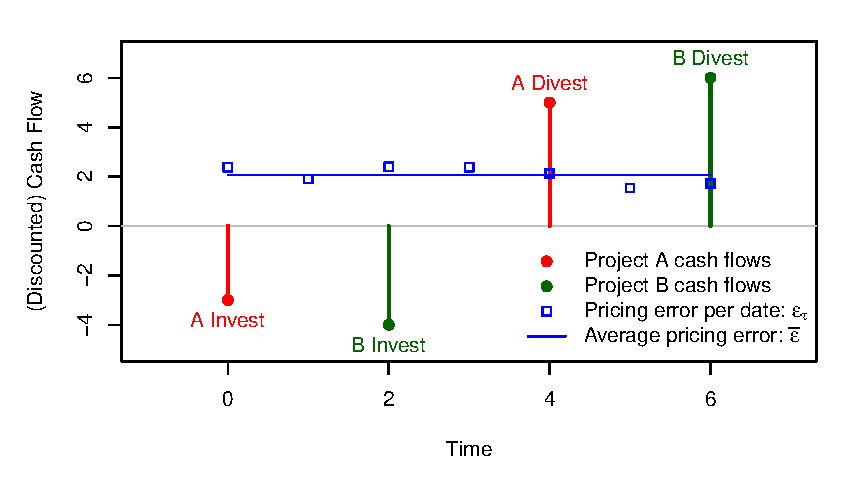
\includegraphics[width=0.9\textwidth]{Figures/spatial/npvs3.eps}
	\caption{
		How to calculate and interpret the average pricing error?
		The time index $t$ is relevant for the net cash flows (black dots).
		The time index $\tau$ is used for the pricing error, i.e., the sum of discounted net cash flows (blue boxes).
		The weighted average of these "pricing errors" gives the average pricing error $\bar{\epsilon}$ as defined in Equation \ref{eq:average_pricing_error} (solid blue line).
		In this example, $\mathrm{card}(\mathcal{T}_{i})=7$, i.e., the number of blue boxes.
	}
	\label{fig:npvs}
\end{figure}

\subsection{Cross-sectional unit: individual fund vs.\ portfolio of funds}
\label{sec:cross_sectional_unit}

According to the classical value-additivity assumption in \cite{HR87}, SDF models invariably shall hold for all pooled or unpooled assets.
As discussed in Subsection \ref{sec:asset_pricing_pooled}, it is best to use the underlying deals as test assets for SDF estimation to avoid the bias terms caused by pooled fund cash flows.
For the second best alternative, it is theoretically not important if the test assets for our SDF are portfolio or individual fund cash flows when the investment dates are the same (see Corollary
\ref{cor:same_investment_dates}).
Empirically it makes a difference, and there are arguments both for and against portfolio formation.

In the risk premium literature, portfolio formation mainly helps to attenuate the errors-in-variables bias connected to two-pass asset pricing methods \citep{JNPR19,PRS19}.
As this is no issue in our case, we could use individual funds.
\cite{C11} argues that portfolio sorting (seen as an auxiliary nonparametric regression that imposes linearity on the relationship between returns and characteristics) shall be replaced by multivariate panel models due to the curse of dimensionality.
Following the same nonparametric regression viewpoint, \cite{CCF19} derive a nonparametric framework where the optimal number of portfolio sorts acts as a data-dependent tuning parameter that grows with sample size.
Generally, the larger the portfolios, the easier any given SDF can price their cash flows since fewer test assets remain.

In the case of private equity funds, the pooling of fund cash flows helps to counter GP financial engineering\footnote{GPs may use bridge credit facilities below the hurdle rate to boost the fund's internal rate of return. This increases the probability of observing funds with only positive or only negative cash flows. However, we want to avoid (the possibility of) cross-sectional units that exhibit just cash flows with the same algebraic sign. Realistic SDFs never can price these cash flow streams.}, which might both change and mask the true risk profile of observed LP cash flows.
Especially for private equity funds, portfolio formation based on vintage years is compelling due to its time-series-like indexing as done by \cite{DLP12}.
This procedure also offers substantial computational benefits as it drastically decreases the number of cross-sectional units.
Further, as stated in \cite{ALS20}, portfolio formation allows more precise factor loading estimates due to decreasing idiosyncratic risk, but at the expense of sacrificing cross-sectional information.
Finally, small (or fixed) $T$ and large $N$ set-ups may face finite sample problems \citep{RRZ20}.
\begin{assume}
	\label{as:portfolio}
	For each vintage year, we pool fund cash flows to form $n_v$ portfolios that serve as cross-sectional units.
	Thus, $n = \sum_{v=1}^V n_v$.
	The two boundary cases are (i) single fund portfolios and (ii) just one portfolio per vintage year. 
\end{assume}
Without loss of generality, we refer to our cross-sectional units as funds, although this corresponds to a special case of our portfolio concept.
In the simulation study in Subsection \ref{sec:simulation_study}, we compare both boundary cases (i) individual funds and (ii) vintage year portfolios.

Thinking more broadly, we could even imagine more extreme boundary cases: 
(iii) on the one hand, we could pool \emph{all} fund cash flows to form only \emph{one} global moment condition for private equity similar to \cite{KN16} and accept potential under-identification; 
(iv) on the other hand, we could operate on underlying deal level like \cite{B14,B16a,B16b} and use gross-of-fee cash flows.

\subsection{Asymptotic framework}
\label{sec:asymptotic_framework}

To allow for multiple funds from the same vintage year in Assumption \ref{as:portfolio}, we employ an auxiliary ``spatial" notion as originally proposed by \cite{KN16}.
The spatial viewpoint is only a technical means to switch from time-series-like to more panel-data-like indexing.
Unlike typical panel data, we do not follow multiple subjects over time, but for each point in time, we exclusively observe multiple new cross-sectional units (i.e., funds from that vintage year).
This unusual two-dimensional indexing causes problems in the PE literature as it neatly fits neither in the (i) time-series, (ii) cross-sectional, nor (iii) panel data literature.
Thus, we generally consider $\bar{\epsilon}$ from Equation \ref{eq:average_pricing_error} as random field (cf. Figure  \ref{fig:randomfields}).
In our case, it is convenient to interpret the fund vintage year $v_i$ as second dimension in our pricing error random field, i.e., $\bar{\epsilon}_{i} \equiv \bar{\epsilon}_{i, v_i}$.
`
Yet, in this section, we mainly follow the time-series asymptotic framework of \cite{PP97} since our ``spatial" distance measure (between vintage years) is time, and adaption to our case is thus straightforward.
If we observe only one fund per vintage year (or, equivalently, form vintage year portfolios), we will easily see that the framework of \cite{PP97} with time-series indexing can be applied without any major modification.


\subsubsection{Vintage year asymptotics}

We assume that the ``spatial" (i.e., economic) distance between cross-sectional units, i.e., private equity funds/portfolios, can be measured quantitatively\footnote{Generally, the economic distance measure could include multiple dimensions, e.g., temporal, geographic, and industry sector proximity. This could be an interesting topic for future research.}.
Our "cross-sectional" asymptotic theory lets the number of funds go to infinity $n \to \infty$.
% However, empirical identification of model parameters requires a sufficient number of funds from different vintage years in the fund-level data set used for model estimation, as emphasized by \cite{DLP12} and \cite{KN16}.
To expose our SDF to many distinct covariate realizations (economic conditions), we also want the number of vintages to increase asymptotically.
\begin{assume}
	\label{as:vya}
	Vintage year asymptotics:
	\begin{enumerate}
		\item The number of vintage years $V \to \infty$ as $n \to \infty$.
		\item The number of funds per vintage year is bounded by some positive constant.
		\item The maximal fund lifetime is also bounded by a positive constant.
		\item The economic distance between fund $i$ and $j$ is measured by the vintage year difference $d_{i,j} = | v_i - v_j | +  \rho_0 1_{i \neq j}$ with minimum distance $\rho_0 > 0$.
	\end{enumerate}
\end{assume}
In terms of the spatial estimation literature, this assumption postulates increasing domain asymptotics and rules out so-called infill asymptotics (cf.\ Figure \ref{fig:randomfields}).
The minimum distance term $\rho_0$ is a means to ensure these increasing domain asymptotics \cite[Assumption 1]{JP12}.
Infill asymptotics corresponds to the assumption of \cite{DLP12} that the number of funds per vintage tends to infinity.

\begin{figure}[ht]
	\centering
	\includegraphics[width=0.9\textwidth]{Figures/spatial/randomfields.pdf}
	\caption{
		Visualization of generic random field types.
		Each black dot marks a different observation $i$ of the cash flow data.
		Importantly, the time axis does \textbf{not} correspond to the index $t$ in $CF_{t,i}$ (rather to vintage years $v_i$).
		Comparing the four choices, we want to avoid an infill random field but prefer our data to constitute an increasing domain random field.
		The infill random field is even asymptotically ``too clustered" or better ``too unrepresentative" to allow for meaningful estimation and inference.
		The time-series and cross-sectional random fields correspond to the standard cases in the literature but could turn out too restrictive for a general approach.
		By smart design (like portfolio formation), we often can map an increasing domain random field to simpler time-series or cross-sectional versions.
	}
	\label{fig:randomfields}
\end{figure}

GMM estimators typically have a fixed number of moment conditions.
Thus, GMM estimators, where the number of moment conditions is allowed to grow with sample size, require special attention \citep{HP06,NW09}.
In many cases, it is probably most convenient to limit the maximum to a finite number of moment conditions (i.e., not each vintage year should form a moment condition).
In this paper, we employ nonlinear least squares estimators since they do not suffer from this ``number of moment condition" issue.


\subsubsection{Law of large numbers}

The global moment condition underlying our estimation approach is that the expected value of $\bar{\epsilon}$ shall be as close as possible to zero if we use the optimal SDF parameter $\theta_0$ (it is nonzero due to Proposition \ref{theo:pooled_bias}). 
To approach this expected value, we rely on a spatial (cross-sectional) law of large numbers instead of applying a time-series law of large numbers.
Here, we want to explicitly acknowledge the statistical dependence of pricing errors from adjacent vintage years.

\begin{assume}
	\label{as:lln}
	Uniform Law of Large Numbers (ULLN) for random fields \cite[Equation 6]{JP09}: \\
	The (i) time-trend and (ii) dependence structure of $\bar{\epsilon}$ shall allow
	\[
	\sup_{\theta \in \Theta} \left| Q_n(\theta) -  \mathbb{E} \left[ Q_n(\theta) \right] 
	\right| \xrightarrow{p.} 0
	\quad {as} \quad n \to \infty
	\]
	where $Q_n(\theta)$ is given by Equation \ref{eq:estimator}.
\end{assume}
Specifically, we could assume (as a so-called primitive condition) the random field $\bar{\epsilon}$ to be spatial near-epoch dependent with respect to fund vintage years \citep{JP09,JP12}, i.e., two funds with distance $d_{i,j}>D$ are assumed to be independent.
	
To satisfy the time trend part (i) of this law of large number assumption, the weighting factor $w$, introduced in Equation \ref{eq:average_pricing_error}, can be used to make $\bar{\epsilon}$ stationary.
Spatial near-epoch dependence with respect to fund vintage years formalizes the simple idea that two fund pricing errors $\bar{\epsilon}$ with a small absolute vintage year difference are supposed to be dependent since they are exposed to the same macroeconomic conditions.
In contrast, two funds with a large absolute vintage year difference can be assumed independent.


\subsubsection{Consistency}

The estimator $\hat{\theta}$ shall converge in probability to the true parameter value $\theta_0$ as the number of distinct vintage years in our data set goes to infinity.
Multiple funds for a specific vintage year are not necessarily required but provide additional information that we want to exploit if available.

\begin{lemma}
	\label{lem:consistency}
	A modified version of \citep[Theorem 2.1]{NM94} holds, i.e.,
	if there is a function $Q_0(\theta)$ such that 
	\begin{enumerate}
		\item Identification: $Q_0(\theta)$ is uniquely minimized at $\theta_0$,
		\item Boundedness: $\Theta$ is compact,
		\item Continuity: $Q_0(\theta)$ is continuous,
		\item Uniform convergence: $\hat{Q}_n(\theta)$ converges uniformly in probability to $Q_0(\theta)$,
	\end{enumerate}
	then $\hat{\theta} \xrightarrow{p} \theta_0$ as $n \rightarrow \infty$.
\end{lemma}

\begin{proof}
	The general proof is given in \cite[Chapter 2]{NM94} for a $\max$ instead of $\min$ extremum estimator.
	Thus, we only recapitulate the four conditions required by the lemma in our specific context.
	\begin{enumerate}
		\item 
		Obviously, we have to replace ``maximized at $\theta_0$" by ``minimized at $\theta_0$" compared to the exposition of \cite[Chapter 2]{NM94}.
		Then, we need to first show that $\mathbb{E} \left[ \bar{\epsilon} (\theta_0) \right] = x$, where $x$ is the minimum bias achievable, see Proposition \ref{theo:pooled_bias}.
		Secondly, we know $Q_0(\theta_0) = \mathbb{E} \left[ L \left( \bar{\epsilon} (\theta_0) \right) \right] \geq 0$, e.g., for $L(x)=x^2$ we have $Q_0(\theta) = \mathbb{E} \left[ \left( \bar{\epsilon} (\theta) \right)^2 \right] = \mathrm{Var} \left[ \bar{\epsilon} (\theta) \right] +  \left( \mathbb{E} \left[ \bar{\epsilon} (\theta) \right] \right)^2 $ where the second summand can be perceived as bias term that is zero for $\theta_0$.
		The variance term $\mathrm{Var} \left[ \bar{\epsilon} (\theta) \right]$ for a simplified DGP is analyzed by Corollary \ref{coro:epsilon_variance_bounds}.
		\item 
		Compactness of $\Theta$ can be assured by lower and upper bounds for all parameters that can be justified by economic reasoning. 
		In our case, e.g., a market beta factor of ten seems implausible for PE funds because of the implied risk and return expectations.
		\item 
		Continuity of the limit is a quiet weak and thus a standard regularity condition.
		\item 
		The second standard regularity condition is given by Assumption \ref{as:lln} which satisfies the definition of uniform convergence in probability \cite[Section 2.1]{NM94} . 
		To make this obvious, we can write $\hat{Q}_n(\theta) = Q_n(\theta) = n^{-1} \sum_{i=1}^n L \left( \bar{\epsilon}_i \right)$ and $Q_0(\theta) = \mathbb{E} \left[ Q_n(\theta) \right]$ and compare it to Assumption \ref{as:lln}.
	\end{enumerate}
	$\square$
\end{proof}


\subsubsection{Central limit theorem}

To assess the large-sample significance of our parameter estimates (as done in the following Subsection \ref{sec:asymptotic_inference}), we want to describe the asymptotic distribution of the parameter vector as a normal distribution.

\begin{proposition}
	\label{prop:clt}
	With estimator consistency established in Lemma \ref{lem:consistency}, and the five (technical) conditions from \cite[Theorem 3.1]{NM94} satisfied, it holds
	\begin{enumerate}
		\item $\sqrt{n}(\hat{\theta} - \theta_0) \overset{d}{\to} \mathcal{N}(0,{\Sigma})$ as $V,n \to \infty$ with covariance matrix ${\Sigma}$, and
		\item The covariance matrix ${\Sigma}$ can be characterized by \citet[Theorem 11.2.b, Theorem H.1]{PP97} (as outlined in the next Section \ref{sec:asymptotic_inference}).
	\end{enumerate}
\end{proposition}

\begin{proof}
	The extended proof of Proposition \ref{prop:clt} may be derived in analogy to the GMM case in \cite[Theorem 4]{JP12} that shows that the general structure of the \cite{PP97} framework also applies to the spatial near-epoch dependent case.
	Alternatively (and easier), the estimator from Equation \ref{eq:estimator} can be clearly formulated as extremum estimator in alignment with our Definition \ref{def:extremum_estimator}.
	In consequence, \cite[Theorem 3.1]{NM94}, which generally describes the asymptotic normality of extremum estimators, is directly applicable to obtain the stated result.
	Thus, all details of the proof can be found in the original reference \cite[Chapter 3]{NM94}.
	$\square$
\end{proof}



\subsection{Large sample inference}
\label{sec:asymptotic_inference}

In this subsection, we demonstrate how to empirically apply Proposition \ref{prop:clt} to obtain the asymptotic standard errors for our estimator from Equation \ref{eq:estimator}.
In the time-series, near-epoch-dependent LMD literature, the covariance matrix ${\Sigma}$ can be characterized according to \citet[Theorem 11.2.b, Theorem H.1]{PP97}:
\[
{\Sigma} = H^{-1} \Lambda (H^{-1})^\top
\]
with expected Hessian matrix converging to $H$ as $n \to \infty$
\[
\mathbb{E}
\left[
\nabla_{\theta \theta} Q_n
\right]
\overset{p}{\to}
H
\]
and the expected covariance matrix of gradients converging to $\Lambda$ as $n \to \infty$
\[
n \cdot \mathbb{E}
\left[
\nabla_{\theta} Q_n
(\nabla_{\theta} Q_n)^\top
\right]
\overset{p}{\to}
\Lambda
\]
Here, the gradient vector $\nabla_{\theta} Q_n$ is denoted as column vector.
We define the corresponding finite sample estimators analogously to \citet[Chapters 12, 13.1]{PP97}, and numerically approximate the first and second partial derivatives by finite differences\footnote{As an alternative to finite differences the widespread Broyden-Fletcher-Goldfarb-Shanno (BFGS) algorithm can be applied to approximate the Hessian \cite[Section 6.1]{NW06}.}.
Specifically, we use the following central difference approximations (with "small" $\delta$) \cite[Algorithm 2]{E17}:
% https://espace.curtin.edu.au/bitstream/handle/20.500.11937/70491/Eu%20C%202017.pdf?sequence=1&isAllowed=y
\[
f_{x}(x,y) \approx \frac{f(x+\delta,y) - f(x-\delta,y)}{2\delta}
\]
\[
f_{xx}(x,y) \approx \frac{f(x+\delta,y) + f(x-\delta,y) - 2  f(x,y)}{\delta^2}
\]
\[
f_{xy}(x,y) \approx \frac{f(x+\delta,y+\delta) + f(x-\delta,y-\delta) -  f(x+\delta,y-\delta) - f(x-\delta,y+\delta)}{4\delta^2}
\]
The Hessian term $\hat{H}$ is relatively straightforward
\[
\hat{H} = \frac{1}{n} \sum_{i=1}^n \nabla_{\theta \theta} L \left( \epsilon_i \right)
\]
Due to the spatial near-epoch dependence, the involved and computationally expensive part is to consistently estimate $\hat{\Lambda}$ by a Spatial Heteroskedasticity and Autocorrelation Consistent (SHAC) covariance matrix estimator \cite[Equation 2]{KS11}
\begin{equation}
\label{eq:hac}
\hat{\Lambda} = \frac{1}{n} \sum_{i=1}^n \sum_{j=1}^n
k_{i,j}
\left[
\nabla_{\theta} L \left( \epsilon_i \right)
\left(
\nabla_{\theta} L \left( \epsilon_j \right)
\right)^\top
\right]
\end{equation}
We define the kernel weight $k$ as
\[
k_{i,j} \equiv K \left( \frac{d_{i,j}}{b_n} \right)
\]
with kernel function $K: \mathbb{R} \to [0,1]$ satisfies $K(0)=1$, $K(x)=K(-x)$, $\int_{-\infty}^{\infty} K^2(x) dx < \infty$, and $K(\cdot)$ continuous at zero and at all but a finite number of other points.
A common choice is the Bartlett kernel $K_{BT}(x)= \max(0, 1-|x|)$; see equation 2.7 in \cite{A91} for other popular kernel choices.
This means absolute vintage year differences larger than the bandwidth (or truncation) parameter $b_n=D$ are considered independent and are thus excluded from the $\hat{\Lambda}$ estimation formula.

In large samples, the vector of parameter standard errors can thus be estimated by
\begin{equation}
	\label{eq:asy_se}
	\mathrm{SE}(\hat{\theta}) = 
	\sqrt{
		\mathrm{diag} \left[
		n^{-\frac{1}{2}}
		\hat{H}^{-1} \hat{\Lambda} (\hat{H}^{-1})^\top
		(n^{-\frac{1}{2}})^\top
		\right] 
	}
	=
	\sqrt{
		\mathrm{diag} \left[
		\hat{H}^{-1} \hat{\Lambda} (\hat{H}^{-1})^\top
		\right] 
		\cdot \frac{1}{n}
	}
\end{equation}
The Wald test statistic for linear hypotheses $H_0: R \theta = r$ and $H_1: R \theta \neq r$ is constructed as (where, $H_0$ and $H_1$ are hypotheses and not Hessian terms $H$)
\[
W = 
(R \hat{\theta} - r)^\top
\left[
R
\frac{\hat{H}^{-1} \hat{\Lambda} (\hat{H}^{-1})^\top}{n}
R^\top
\right]^{-1}
(R \hat{\theta} - r)
\stackrel{H_0}{\sim}
\chi_q^2
\]
where $\hat{\theta}$ is the $p \times 1$ parameter vector, $R$ is a $q \times p$ matrix, and $r$ is a $q \times 1$ vector.
Usually, we select $R$ as $p \times p$ identity matrix, and $r$ as $p \times 1$ vector (e.g., of zeros).
Under the null hypothesis, $W$ is chi-squared distributed with $q$ degrees of freedom. As large values of $W$ indicate the rejection of $H_0$, the corresponding p-value is calculated as $1 - F_{\chi_q^2}(W)$ where $F_{\chi_q^2}$ is the cumulative distribution function of a chi-squared random variable with $q$ degrees of freedom.

However, given the limited amount of available private equity data (typically the oldest vintages start in the 1980s), asymptotic characterizations of ${\Sigma}$ and $\mathrm{SE}(\hat{\theta})$ are of limited importance. 
In empirical applications, the small sample behavior of an estimation method for private equity data is more relevant than its asymptotic theory.
Moreover, the standard asymptotic distribution associated with an estimator is generally not valid for post-model-selection inference, i.e., if a model selection procedure is applied to find the best model from a collection of competitors \citep{LP05}.





\subsection{Comparison to similar estimators}
\label{sec:comparison_to_similar_estimators}

Our Least-Mean-Distance (LMD) estimator introduced in Section \ref{sec:fundwise_lmd_estimator} belongs to the class of semiparametric nonlinear M-estimators as defined in \cite{PP97} which are extremum estimators.
To gain more flexibility and avoid unneeded complexity, we intentionally opt against the most prominent semiparametric nonlinear M-estimator framework, i.e., classical time-series Generalized Method of Moments (GMM) \citep{H82,H12}.
A classical GMM approach requires the construction of stationary, ergodic time-series of moment conditions that are used to empirically estimate the expected value of pricing errors in Equation \ref{eq:pricing_error}.
The stationarity requirement of classical time-series GMM limits (i) more elaborate weighting schemes for $w$, like fund-size weighting, and (ii) the usage of fund cash flows from non-realized vintages.

\subsubsection{Comparison to \cite{DLP12}}

The \cite{DLP12} approach is most closely related to our methodology.

One important difference is that we select a simpler and more flexible LMD estimator instead of a cross-sectional GMM approach.
In our view, the choice of the more complex cross-sectional GMM just causes some conceptional issues, whereas the underlying formulas are basically the same as for our LMD estimator\footnote{The formulas are this similar because \cite{DLP12} use the identity matrix as GMM weighting matrix and skip the second GMM step.}.
As a first limitation, they have to regard vintage-year portfolios as their cross-sectional units; we can also use individual funds.
In this context, we also question their statement that ``to identify $\beta$, it is essential that the different FoFs are exposed to different market returns" since it is perfectly fine to perceive their estimator as cross-sectional approach\footnote{In a classic cross-sectional regression, we only have one market return realization.}.
Second, the \cite{DLP12} asymptotic theory assumes the number of funds (or deals) per vintage year portfolio to go to infinity.
To comply with standard GMM assumptions, the number of vintage years, which corresponds to the number of moment conditions in their approach, \emph{must be considered fixed} and thus cannot grow asymptotically \citep{HP06,NW09}.
For a typical LMD estimator (e.g., nonlinear least squares), this constraint does not exist.
Our asymptotic theory lets both (i) the number of vintage years and (ii) the number of funds go to infinity but bounds the number of funds per vintage year.

Further, \cite{DLP12} discount all fund cash flows just to the first cash flow date (like in a classical net present value calculation).
In contrast, we additionally average over all dates within $\mathcal{T}_{i}$ to tackle the problem arising from pricing pooled cash flows, which we thoroughly analyzed in subsection \ref{sec:asset_pricing_pooled}.
Although \cite{DLP12} describe their estimator as a one-step GMM approach, we consider it a special case of our LMD estimator.
Specifically, Equation \ref{eq:estimator} from our methodology is a generalization of equation 3 from their paper.
Consequently, if someone accepts the assumptions from Subsection \ref{sec:asymptotic_framework}, our large sample inference framework from Subsection \ref{sec:asymptotic_inference} applies to their case without any significant modification.
Finally, \cite{DLP12} apply simple cross-sectional bootstrapping to obtain standard errors; in contrast, in Subsection \ref{sec:model_selection}, we use a cross-validation technique that is adapted to the near-epoch dependence of the PE fund data.

\subsubsection{Comparison to \cite{KN16}}

\cite{KN16}, first of all, realized the usefulness of employing an auxiliary spatial framework to establish asymptotic inference results for a fund-level panel dataset of private equity funds.
To account for the cross-sectional dependence between funds, they measure the economic distance between two private equity funds (by the degree of cash flow overlap).
Concretely, their asymptotic inference framework draws on the spatial HAC estimator of \cite{C99}; our spatial HAC framework uses \cite{PP97,KS11,JP12}.
However, they ultimately utilize a classical GMM estimator, thus a time-series law of large numbers.
Specifically, we obtain the estimator of \cite[Equation 18]{KN16} in our framework if we replace $Q_n(\theta)$ in Equation \ref{eq:estimator} by Equation \ref{eq:kn16_estimator}.
\begin{equation}
\label{eq:kn16_estimator}
Q_n(\theta) = 
L \left(
\frac{1}{n}
\sum_{i=1}^n
\bar{\epsilon}_{i} 
\right)
\quad
\mathrm{with}
\quad
L(x) = x^{\top} W x = x^{\top} I x
\end{equation}
with identity matrix $I$ as weighting matrix $W$.
In accordance with classical GMM, the function $\frac{1}{n} \sum_{i=1}^n \bar{\epsilon}_{i}: \mathbb{R}^{n \times T} \times \Theta \to \mathbb{R}^m$ should be perceived as multidimensional where the dimensionality of the function output corresponds to the number of moment conditions.

Time-series GMM estimators inherently bear the risk of under-identification if the corresponding time-series is constructed by pooling all fund cash flows from a given fund type.
Exactly this happens in Equation \ref{eq:kn16_estimator} with $m=1$ where we consequentially obtain a GMM estimator with just one moment condition\footnote{In contrast, our estimator corresponds to the opposite edge case with asymptotically an infinite number of LMD ''moment conditions" (units to price) as we let $n \to \infty$.}.
To counter under-identification, additional characteristic-based fund portfolios could be formed to increase the number of moment conditions per fund type; also, random portfolios combined with bootstrapping could make sense.
Yet, \cite{KN16} take another approach and introduce the concept of Generalized Public Market Equivalent (GPME), which elegantly avoids the under-identification issue.
Firstly, a public market SDF model is estimated by pricing public trading strategies that shall replicate PE funds instead of directly pricing the observed PE fund cash flows.
Only in a second step these public market SDF models are applied to evaluate private equity fund cash flows.

Given these differences, our approach may not be perceived as a straightforward generalization of the \cite{KN16} framework.
In contrast, our LMD estimator generalizes the \cite{DLP12} method. 
Table \ref{tab:comparison} summarizes the most prominent distinctions between the three approaches.

\begin{table}[ht]
	\centering
	\resizebox{0.9\textwidth}{!}{%
		\begin{tabular}{llll}
			& \cite{DLP12} & \cite{KN16} & Our approach \\ 
			\hline
			\hline
			M-estimator & Cross-sectional Generalized & Time-series Generalized  & Least-Mean-  \\
			& Method of Moments & Method of Moments & Distance \\
			\hline
			Pricing error averaging & No & No & Yes \\
			\hline
			Cash flows priced & PE cash flows & public cash flows & PE cash flows \\
			\hline
			Asymptotics & cross-sectional & time-series & spatial \\
			& \#funds $\to \infty$ & \#vintages $\to \infty$ & \# of both $\to \infty$ \\
			\hline
			Inference & bootstrap & spatial HAC & cross-validation \\
			& & & \& spatial HAC \\
			\hline
			Cross-sectional unit & vintage year portfolio & single fund & testing both \\
			\hline
			SDF & simple linear & exponentially affine & testing both \\
			\hline
			\hline
		\end{tabular}
	}
	\caption{Comparison to similar estimation frameworks.} 
	\label{tab:comparison}
\end{table}



\section{Empirical application}
\label{sec:empirical_application}

\subsection{Data}

We use the Preqin cash flow data set as of 26th February 2020 that is well known in the academic private equity literature \citep{HJK14,KN16,ACGP18}.
For an overview of the available asset classes and strategies in the unprepared raw Preqin dataset, see Table  \ref{tab:summary_preqin_strategy}.
After data preparation, we pool all regions and group the remaining funds according to the Preqin asset class classification:
PE ("Private Equity"; 2248 distinct funds in data set; 36 vintage years) and
VC ("Venture Capital"; 871; 36).
%RE ("Real Estate"; 742; 27),
%PD ("Private Debt"; 441; 31),
%INF ("Infrastructure", 144; 17), 
%NR ("Natural Resources", 138; 26).
For these fund types, we extract all (i) equal-weighted and (ii) fund-size-weighted cash flow series.
For non-liquidated funds, we treat the latest net asset value as final cash flow.
We explicitly refrain from excluding the most recent vintage years.
Thus, the minimum vintage year is 1983 (just for PE), and the maximum is 2019.

The public market factors that enter our SDF draw on the US data set of the recently popularized $q^5$ investment factor model sourced from \url{http://global-q.org/factors.html} \citep{HXZ15,HXZ20}. 
Their five-factor model includes the market excess return (MKT), a size factor (ME), an investment factor (IA), a return on equity factor (ROE), and an expected growth factor (EG).

% latex table generated in R 3.4.2 by xtable 1.8-4 package
% Fri Nov 19 08:43:30 2021
\begin{table}[H]
	\centering	
	\begin{tabularx}{0.9\textwidth}{lcXr}
			\hline
			Type & Asset Class & Strategy & Fund Count \\ 
			%\hline
			%Infrastructure & Infrastructure Core &   32 \\ 
			%Infrastructure & Infrastructure Core Plus &   58 \\ 
			%Infrastructure & Infrastructure Debt &   26 \\ 
			%Infrastructure & Infrastructure Fund of Funds &    6 \\ 
			%Infrastructure & Infrastructure Opportunistic &   12 \\ 
			%Infrastructure & Infrastructure Secondaries &    4 \\ 
			%Infrastructure & Infrastructure Value Added &   36 \\ 
			%\hline
			%Natural Resources & Energy &    2 \\ 
			%Natural Resources & Natural Resources &  146 \\ 
			%Natural Resources & Timber &   19 \\ 
			%\hline
			%Private Debt & Direct Lending &    3 \\ 
			%Private Debt & Direct Lending - Blended / Opportunistic Debt &   21 \\ 
			%Private Debt & Direct Lending - Junior / Subordinated Debt &    9 \\ 
			%Private Debt & Direct Lending - Senior Debt &   89 \\ 
			%Private Debt & Direct Lending - Unitranche Debt &    4 \\ 
			%Private Debt & Distressed Debt &  153 \\ 
			%Private Debt & Mezzanine &  147 \\ 
			%Private Debt & Private Debt Fund of Funds &    4 \\ 
			%Private Debt & Special Situations &   58 \\ 
			\hline
			PE & Private Equity & Balanced &   63 \\ 
			PE & Private Equity & Buyout & 1251 \\ 
			PE & Private Equity & Co-Investment &   75 \\ 
			PE & Private Equity & Co-Investment Multi-Manager &   58 \\ 
			PE & Private Equity & Direct Secondaries &   24 \\ 
			PE & Private Equity & Fund of Funds &  589 \\ 
			PE & Private Equity & Growth &  265 \\ 
			PE & Private Equity & Secondaries &  131 \\ 
			PE & Private Equity & Turnaround &   18 \\ 
			%\hline
			%Real Estate & Real Asset &    1 \\ 
			%Real Estate & Real Estate Co-Investment &   15 \\ 
			%Real Estate & Real Estate Core &   33 \\ 
			%Real Estate & Real Estate Core-Plus &   44 \\ 
			%Real Estate & Real Estate Debt &  106 \\ 
			%Real Estate & Real Estate Distressed &   27 \\ 
			%Real Estate & Real Estate Fund of Funds &   29 \\ 
			%Real Estate & Real Estate Opportunistic &  225 \\ 
			%Real Estate & Real Estate Secondaries &   15 \\ 
			%Real Estate & Real Estate Value Added &  315 \\ 
			\hline
			VC & Venture Capital & Early Stage &  262 \\ 
			VC & Venture Capital & Early Stage: Seed &   42 \\ 
			VC & Venture Capital & Early Stage: Start-up &   37 \\ 
			VC & Venture Capital & Expansion / Late Stage &  110 \\ 
			VC & Venture Capital & Venture (General) &  513 \\ 
			VC & Venture Capital & Venture Debt &   21 \\ 
			\hline
	\end{tabularx}
	\caption{Summary of asset classes and strategies in the unprepared raw Preqin dataset.} 
	\label{tab:summary_preqin_strategy}
\end{table}

\subsection{Model and estimator specifications}
\label{sec:model_selection}

We test a simple linear SDF model similar to \cite{DLP12}
\begin{equation}
\label{eq:linear_sdf}
\Psi_{\tau,t}^{\mathrm{SL}} (\theta) = 
\frac{\prod_{h=0}^{\tau}\ \left(1 + \alpha + r_{h} + \sum_j\ \beta_j \ F_{j,h} \right)}{\prod_{h=0}^{t}\ \left(1 + \alpha + r_{h} + \sum_j\ \beta_j\ F_{j,h} \right)}
\end{equation}
and an exponential affine SDF model adapted from \cite{KN16}
\begin{equation}
\label{eq:expaff_SDF}
\Psi_{\tau,t}^{\mathrm{EA}} (\theta) = 
\exp
\left[
\sum_{h=0}^{\tau} X_h
\sum_{h=0}^{t} - X_h
\right]
\end{equation}
with
\[
X_h = \alpha + \log (1 + r_h) + \sum_{j \in J} \beta_{j} \cdot \log (1 + F_{j,h})
\]
with (arithmetic) risk-free return $r=R_{rf}-1$, (arithmetic) zero-net-investment portfolio returns $F_j$, and parameter vector $\theta=(\alpha,\beta)$.
To avoid overfitting, we just test six simple SDF models that contain \{MKT\} alone or \{MKT\} plus \{ME or IA or ROE or EG or Alpha\}.
In Equation \ref{eq:estimator}, we use the quadratic loss function $L(x)=x^2$.

To assess the parameter significance, we compute the asymptotic standard errors as outlined in Subsection \ref{sec:asymptotic_inference}.
For the Bartlett kernel's bandwidth $b_n=D$ we select 12 years, i.e., funds with absolute vintage year differences larger than 12 years are assumed to be independent.

Additionally, we want to test the finite - or, more honestly, small - sample parameter significance and the out-of-sample performance of our SDF models.
To account for the dependency between funds from adjacent vintage years caused by overlapping fund cash flows, we draw on $hv$-block cross-validation \citep{R00}.
Therefore, we form three partitions for several vintage year groups.
As larger validation sets are preferred for model selection, the validation set ($v$-block) always contains funds of three neighboring vintage years (e.g., 2000, 2001, 2002).
To reduce the dependency between training and validation set, we remove all funds from three-year-adjacent vintage years, i.e., the $h$-block (e.g., 1997, 1998, 1999, 2003, 2004, 2005).
Funds from the remaining vintage years enter the training set and are thus used for model estimation (e.g., 1985-1996, 2006-2019).
We apply ten-fold cross validation using the ten validation sets described in Table \ref{tab:hv_block_cv}.
This means we replace the bootstrap standard error calculation of \cite{DLP12} by $hv$-block cross-validation since the new method (i) accounts for near-epoch-dependence, (ii) focuses directly on the out-of-sample performance of the SDF models, and (iii) is computationally cheaper.

\begin{table}[ht]
	\centering
	\resizebox{0.9\textwidth}{!}{%
	\begin{tabular}{lllll}
		training.before & $h$-block.before & $v$-block & $h$-block.after & training.after \\ 
		\hline
		estimation & remove & validation & remove & estimation \\ 
		\hline
		\hline
		start-1984 & 1985,1986,1987 & 1988,1989,1990 & 1991,1992,1993 & 1994-end \\ 
		start-1987 & 1988,1989,1990 & 1991,1992,1993 & 1994,1995,1996 & 1997-end \\ 
		start-1990 & 1991,1992,1993 & 1994,1995,1996 & 1997,1998,1999 & 2000-end \\ 
		start-1993 & 1994,1995,1996 & 1997,1998,1999 & 2000,2001,2002 & 2003-end \\ 
		start-1996 & 1997,1998,1999 & 2000,2001,2002 & 2003,2004,2005 & 2006-end \\ 
		start-1999 & 2000,2001,2002 & 2003,2004,2005 & 2006,2007,2008 & 2009-end \\ 
		start-2002 & 2003,2004,2005 & 2006,2007,2008 & 2009,2010,2011 & 2012-end \\ 
		start-2005 & 2006,2007,2008 & 2009,2010,2011 & 2012,2013,2014 & 2015-end \\ 
		start-2008 & 2009,2010,2011 & 2012,2013,2014 & 2015,2016,2017 & 2018-end \\ 
		start-2011 & 2012,2013,2014 & 2015,2016,2017 & 2018,2019,2020 & 2021-end \\ 
		\hline
		\hline
	\end{tabular}
	}
	\caption{Partitions used for $hv$-block cross-validation.}
	\label{tab:hv_block_cv}
\end{table}


\subsection{Simulation study}
\label{sec:simulation_study}

Our Monte Carlo experiments examine the following questions related to the bias and variance of our estimation methodology in finite samples.\footnote{As each simulation study it more investigates the ability to identify the assumed data generating process than the corresponding SDF model.}
Is it beneficial to use vintage-year portfolios instead of individual funds?
Which SDF model performs better when we also use the corresponding data generating process (i.e., assume correct model specification)?
How is estimator precision affected by varying numbers of vintage years and cross-sectional units?
Which is the optimal set of discounting dates $\mathcal{T}$?


We use historical $q$-investment factors from 1986 to 2005 and simulate 20 funds for each of these 20 vintage years.
Each fund contains 15 deals with equal investment amounts and exactly one divestment cash flow.
Deals are entered within the first five years of the fund lifetime following a discrete uniform distribution and afterward held between one to ten years again uniformly distributed.
The deal returns are generated by the simple linear or exponential affine SDF models described in Equations \ref{eq:linear_sdf} and \ref{eq:expaff_SDF}.
In the base case, we just use the MKT factor with $\beta_{\mathrm{MKT}}=1$ and in each month, add a normal i.i.d. error term with standard deviation $\sigma=0.2$ and zero mean.
Additionally, we test an intercept term $\alpha$ of -0.25\% per month and a high $\beta_{\mathrm{MKT}}$ of 2.5.
In the exponential affine case, we adjust the lognormally distributed error mean to zero by subtracting $0.5 \sigma^2$.
If a negative return exceeds -100\%, the company defaults with a zero exit cash flow.
In contrast, the error term in the simulations of \cite{DLP12} is more well-behaved as it follows a shifted lognormal distribution that, even with arbitrarily high error term variance, just allows for returns below say -99\%, if the market return is close to its lower bound (see equation 9 in their online appendix).
In our base case, the set of discounting dates $\mathcal{T}$ contains all months from the first cash flow to the maximum month 180.
To assess our estimator's bias and variance, we simulate 1000 test scenarios for vintage year portfolios and only 200 test cases when using individual funds due to the higher computational costs of simulating the individual fund cash flows.


\paragraph{Cross-sectional unit $i$:}

As presumed in Subsection \ref{sec:cross_sectional_unit}, vintage year portfolio results appear to have lower bias and variance when compared to individual funds.
For the simple linear SDF and maximum month 180, the mean and standard deviation of the coefficient estimate $\hat{\beta}_{\mathrm{MKT}}$ is 1.016 (0.2) for the vintage year portfolio and 1.096 (0.376) for individual funds. 
More results are depicted in Figure \ref{fig:simulation_funds_vs_vyps}.
However, for individual funds, we only simulate 200 iterations due to the high computational cost.

This finding has two important implications:
On the one hand, vintage year portfolio formation can substantially decrease our estimator's bias and variance.
On the other hand, it also dramatically reduces the number of cross-sectional units and consequentially impairs the importance of asymptotic results.
These considerations may explain the choice of \cite{KN16} to use individual funds as cross-sectional units in their asymptotic SHAC framework to obtain smaller standard error estimates.

\begin{figure}
	\centering
	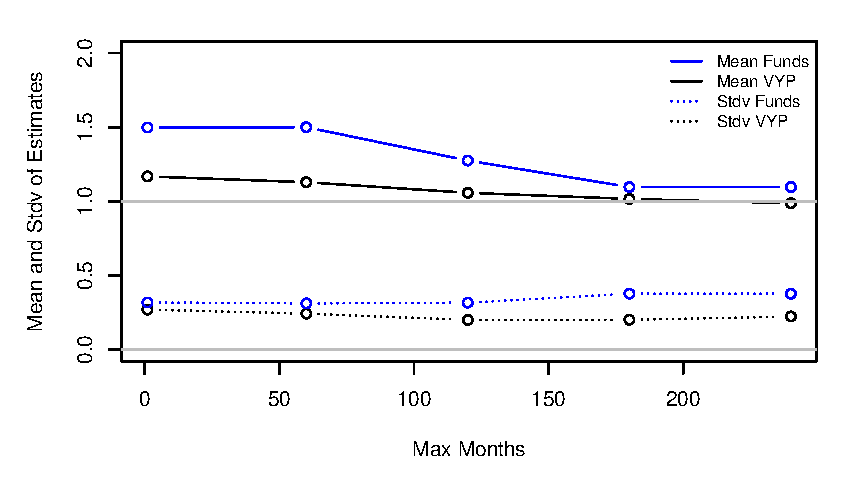
\includegraphics[width=0.9\textwidth]{Figures/spatial/Simulationfundsvsvyps}
	\caption{Simulation results comparing individual funds vs. vintage year portfolios (VYPs) with true $\beta=1$ and simple linear SDF (200 simulation iterations).}
	\label{fig:simulation_funds_vs_vyps}
\end{figure}


\paragraph{SDF model $\Psi$:}

In our base case with vintage year portfolios, the exponential affine SDF shows a mean and standard deviation of 1.011 (0.175) compared to the 1.016 (0.2) achieved by the simple linear SDF.
Generally, the exponential affine SDF model and the simple linear SDF model exhibit similar bias and variance, cf.\ panels A and B in Table \ref{tab:simulation_study}.
Figure \ref{fig:simulation_expaff_vs_simlin} visualizes the true $\beta=1$ case, which shows that the estimation results are not overly sensitive to the choice of the SDF model.

Moreover, the perceived superiority of exponential affine SDFs is probably rather theoretical than practical as other proponents also emphasize their universality mainly from a mathematical perspective without providing supportive empirical or simulation results \citep{GM07,BMP08}.

\begin{figure}
	\centering
	\includegraphics[width=0.9\textwidth]{Figures/spatial/Simulationexpaffvssimlin}
	\caption{Simulation results comparing exponentially affine and simple linear SDF with true $\beta=1$ and vintage year portfolios (1000 simulation iterations).}
	\label{fig:simulation_expaff_vs_simlin}
\end{figure}


\paragraph{Varying vintages $V$ and portfolio sizes $n/V$:}

To test the effect of varying data sizes available for MKT factor estimation, we in/decrease the (i) number of vintage years and (ii) the number of funds per vintage year (cf. Table \ref{tab:simulation_study_size}).
Here we use vintage year portfolios and the simple linear SDF.
For our simple data generating process, increasing the number of deals/funds per vintage year portfolio appears to decrease the estimator's variance more effectively than adding more vintage years.
However, the bias is almost the same for all tested specifications.
Generally, we seem to need many new data points to ensure a reasonable variance of our estimator.

\begin{table}[ht]
	\centering
	\resizebox{0.9\textwidth}{!}{%
	\begin{tabular}{rrrrrrr}
		& Base & Big $n/V$ & Big $V$ & Big $V$ & Small $V$ & Small $V$ \\ 
		\hline
		\hline
		Start vintage & 1986 & 1986 & 1967 & 1967 & 1986 & 1996 \\ 
		End vintage & 2005 & 2005 & 2005 & 2005 & 1995 & 2005 \\ 
		\#Funds per vintage & 20 & 40 & 10 & 20 & 20 & 20 \\ 
		\hline
		Mean $\beta_{\mathrm{MKT}}$ & 1.011 & 1.020 & 0.993 & 1.015 & 1.027 & 0.934 \\ 
		Stdv $\beta_{\mathrm{MKT}}$ & 0.187 & 0.133 & 0.263 & 0.227 & 0.232 & 0.418 \\ 
		\hline
		\hline
	\end{tabular}
	}
	\caption{Simulation study for varying  number of vintages and number of funds per vintage. 
		We use vintage year portfolios, the simple linear SDF with true $\beta_{\mathrm{MKT}}=1$, maximum month 180, and 500 simulation iterations.} 
	\label{tab:simulation_study_size}
\end{table}

\paragraph{Size of set $\mathcal{T}$:}

The results in Table \ref{tab:simulation_study} indicate that we can control the asymptotic bias by an appropriate choice of the set $\mathcal{T}$.
For the one-factor model, the bias almost vanishes when we average over all discounting dates in the maximal fund lifetime of 180 months. 
For smaller or larger sets for $\mathcal{T}$, we find increasing bias terms.
Recall that using the minimal set for $\mathcal{T}$, i.e., discounting all cash flows just to the fund inception date, corresponds exactly to the \cite{DLP12} approach. 
Thus, the original \cite{DLP12} methodology might achieve a suboptimal asymptotic bias since it does not average pricing errors over multiple discounting dates.

The same finding also holds when we limit the maximal fund lifetime to ten years by reducing the maximum deal holding period from ten to five years. 
Here, under correct model specification with $\beta_{\mathrm{MKT}}=1$ , the smallest bias is obtained for maximum month 120, for max. month 60 we get 1.028 (0.116), for max. month 120, we get 1.005 (0.116), and for max. month 180 we get 0.969 (0.13).
However, this simulation results only hold for the one-factor model (MKT) reported here. 
For multi-factor models, smaller max. month values can yield the lowest bias term.
Thus, our simulation study could not reveal a formula how to determine the optimal set of $\mathcal{T}$; it seems to be data and SDF model dependent. 

In Table \ref{tab:simulation_study} for both true and false model specifications, the $\alpha$ standard deviation is very high compared to its mean value.
This may indicate it is rather delicate to empirically determine private equity's historical outperformance by our semiparametric estimator. \newline

To conclude, our simulations study rationalizes two key practices from the \cite{DLP12} paper: (i) vintage year portfolio formation helps to improve estimator precision, and (ii) increasing the number of funds per vintage seems to be more effective in controlling estimator variance that increasing the number of vintages\footnote{Finding (ii) may explain the choice of \cite{DLP12} to employ an asymptotic law that lets the number of deals/funds per vintage tend to infinity.}.
However, our examples with correct specification cannot support the assumption of \cite{KN16} that (iii) the exponential affine SDF is (clearly) superior to the simple liner SDF in a multi-period framework; actually, their bias and variances are quite equal.
Moreover, our simulation study suggests that (iv) averaging pricing errors over multiple dates strikingly reduces the bias inherent to the original procedure of \cite{DLP12} that just discounts all cash flows to the fund inception date.
Actually, choosing the set $\mathcal{T}$ according to the fund lifetime seems to decrease the bias (and to a lesser extent also the variance) more effectively than all other measures combined.

\begin{table}[H]
	\centering
	\resizebox{0.9\textwidth}{!}{%
		\begin{tabular}{lrrrrrr}
			\multicolumn{7}{c}{Panel A: simple linear SDF} \\
			\hline
			Model==DGP & True & \multicolumn{2}{c}{False} & False & \multicolumn{2}{c}{True} \\
			MaxMonth & $\beta=1$ & $\alpha=0$ & $\beta=1$ & $\beta=2.5$ & $\alpha=-0.25$ & $\beta=2.5$ \\ 
			\hline
			\hline
			1 - mean & 1.168 & 1625\% & 0.003 & 2.023 & 5879\% & -16.711 \\ 
			1 - stdv & 0.269 & 2792\% & 9.968 & 0.342 & 866\% & 13.347 \\ 
			\hline
			60 - mean & 1.129 & 0.138\% & 0.933 & 2.103 & -0.086\% & 2.285 \\ 
			60 - stdv & 0.242 & 0.245\% & 0.363 & 0.302 & 0.253\% & 0.406 \\ 
			\hline
			120 - mean & 1.058 & 0.112\% & 0.906 & 2.063 & -0.085\% & 2.239 \\ 
			120 - stdv & 0.200 & 0.214\% & 0.313 & 0.253 & 0.239\% & 0.385 \\ 
			\hline
			180 - mean & 1.016 & 0.041\% & 0.965 & 2.052 & -0.161\% & 2.370 \\ 
			180 - stdv & 0.200 & 0.172\% & 0.334 & 0.277 & 0.173\% & 0.403 \\ 
			\hline
			240 - mean & 0.987 & -0.053\% & 1.077 & 2.072 & -0.277\% & 2.589 \\ 
			240 - stdv & 0.223 & 0.162\% & 0.361 & 0.326 & 0.118\% & 0.375 \\
			\hline 
			300 - mean & 0.946 & -0.149\% & 1.175 & 2.080 & -0.357\% & 2.714 \\ 
			300 - stdv & 0.235 & 0.174\% & 0.377 & 0.398 & 0.114\% & 0.366 \\ 
			\hline
			360 - mean & 0.895 & -0.245\% & 1.269 & 2.048 & -0.461\% & 2.859 \\ 
			360 - stdv & 0.268 & 0.201\% & 0.399 & 0.551 & 0.140\% & 0.386 \\ 
			\hline
			\hline
			\multicolumn{7}{l}{} \\
			\multicolumn{7}{c}{Panel B: exponential affine SDF} \\
			\hline
			Model==DGP & True & \multicolumn{2}{c}{False} & False & \multicolumn{2}{c}{True} \\
			MaxMonth & $\beta=1$ & $\alpha=0$ & $\beta=1$ & $\beta=2.5$ & $\alpha=-0.25$ & $\beta=2.5$ \\ 
			\hline
			\hline
			1 - mean & 1.207 & 203\% & 1.276 & 2.256 & 692\% & 1.704 \\ 
			1 - stdv & 0.344 & 314\% & 0.710 & 0.290 & 13\% & 1.666 \\ 
			\hline
			60 - mean & 1.146 & 0.126\% & 0.941 & 2.264 & -0.018\% & 2.277 \\ 
			60 - stdv & 0.275 & 0.264\% & 0.386 & 0.256 & 0.370\% & 0.473 \\ 
			\hline
			120 - mean & 1.062 & 0.107\% & 0.908 & 2.221 & 0.009\% & 2.205 \\ 
			120 - stdv & 0.200 & 0.237\% & 0.333 & 0.187 & 0.357\% & 0.448 \\ 
			\hline
			180 - mean & 1.011 & 0.027\% & 0.971 & 2.182 & -0.136\% & 2.358 \\ 
			180 - stdv & 0.175 & 0.211\% & 0.366 & 0.168 & 0.344\% & 0.505 \\ 
			\hline
			240 - mean & 0.972 & -0.088\% & 1.095 & 2.144 & -0.441\% & 2.723 \\ 
			240 - stdv & 0.174 & 0.224\% & 0.406 & 0.178 & 0.317\% & 0.503 \\ 
			\hline
			300 - mean & 0.928 & -0.202\% & 1.203 & 2.083 & -0.717\% & 2.985 \\ 
			300 - stdv & 0.181 & 0.253\% & 0.426 & 0.254 & 0.340\% & 0.513 \\ 
			\hline
			360 - mean & 0.874 & -0.319\% & 1.304 & 1.685 & -1.095\% & 3.272 \\ 
			360 - stdv & 0.208 & 0.291\% & 0.447 & 0.772 & 0.374\% & 0.586 \\ 
			\hline
			\hline
		\end{tabular}
	}
	\caption{
		Simulation study to compare the simple linear with the exponential affine SDF and to determine the optimal size of the set $\mathcal{T}$.
		Here, we always use vintage year-portfolios and 1000 simulation iterations.
		For better readability, $\beta_{\mathrm{MKT}}=\beta$.
		For the unity and high beta model, we test true and false model specifications (with and without the monthly $\alpha$ term).
	} 
	\label{tab:simulation_study}
\end{table}

\subsection{Empirical results}

Following the conclusions from the previous subsection, we use vintage-year portfolios to estimate simple linear SDF models with maximum month 180.
Asymptotic inference results for the full dataset are exhibited in Table \ref{tab:ai_180_FW_VYP_SL} for fund-size weighting and in Table \ref{tab:ai_180_EW_VYP_SL} for equal weighting.
The results for $hv$-block cross-validation are displayed in Table \ref{tab:cv_180_FW_VYP_SL} for fund-size weighting and in Table \ref{tab:cv_180_EW_VYP_SL} for equal weighting.
We generally analyze the results in a two-step procedure: For a given model specification, we use the cross-validation error (i.e., the average out-of-sample error) to select the best model for each fund type but analyze the corresponding coefficient estimates from the asymptotic inference tables (estimated on the entire data set).
Therefore, for each fund type the SDF models in the asymptotic inference Tables \ref{tab:ai_180_FW_VYP_SL} and \ref{tab:ai_180_EW_VYP_SL} are sorted by the corresponding cross-validation error.
Throughout this subsection, we define the statistical significance of coefficient estimates in terms of a $t$-ratio $\hat{\theta}[SE(\hat{\theta})]^{-1}$ greater than 1.96.

% latex table generated in R 3.4.2 by xtable 1.8-4 package
% Mon Jun  8 20:27:19 2020
\begin{table}[ht]
	\centering
	\resizebox{0.9\textwidth}{!}{%
	\begin{tabular}{llrrrrrr}
		& & \multicolumn{3}{l}{MKT Factor} & \multicolumn{3}{l}{Second Factor} \\ 
		Weighting & Inference & Coef & SE & SE.indep & Coef & SE & SE.indep \\ 
		\hline
		\hline
		fund-size & asymptotic & 0.75 & 27.06 & 19.73 & 0.80 & 28.95 & 20.94 \\ 
		fund-size & cross-validation & 0.85 & 0.38 & - & 0.59 & 0.51 & - \\ 
		\hline
		equal & asymptotic & 0.76 & 26.75 & 16.16 & 0.76 & 11.25 & 6.69 \\ 
		equal & cross-validation & 0.84 & 0.34 & - & 0.62 & 0.50 & - \\ 
		\hline
		\hline
	\end{tabular}
	}
	\caption{
		Top-level overview over Table \ref{tab:ai_180_FW_VYP_SL} to \ref{tab:cv_180_EW_VYP_SL}: 
		Averages of absolute values of coefficient estimates and standard errors (SEs).
		We see that asymptotic SEs are much higher than the SEs obtained by cross-validation.
	} 
	\label{tab:ai_sum_abs}
\end{table}

Table \ref{tab:ai_sum_abs} helps to get a rough overview of Table \ref{tab:ai_180_FW_VYP_SL} to \ref{tab:cv_180_EW_VYP_SL} as it summarizes their absolute column means.
Conspicuously, asymptotic standard errors (SEs) seem enormously high and, moreover, contain colossal outliers.
The standard errors implied by $hv-$block cross-validation are considerably smaller than the asymptotic SEs and seem to lie within a plausible range.
When just looking at asymptotic standard errors of the second factors, fund-size weighting exhibits substantially larger SEs than fund equal-weighting.
Assuming independence between funds from different vintages decreases asymptotic SEs by approximately 30-40\% compared to a realistic kernel bandwidth of $D=12$.
But even these independent SEs rarely imply statistical significance coefficient estimates with $t$-ratios bigger than 1.96.
In Table \ref{tab:ai_180_FW_VYP_SL} with fund-size weighting, just one out of 36 models exhibit asymptotically significant MKT and second-factor estimates.
In the case of equal-weighting, Table \ref{tab:ai_180_EW_VYP_SL} also shows just one asymptotically significant model out of 36.

In summary, the results reveal weak two-factor models with MKT plus a second $q$-investment factor. 
Likewise, the simulation results from the previous subsection indicate a rather high variance associated with our semiparametric estimator (given the amount of data typically available).
Thus, we recommend focusing on single MKT factor models even when their asymptotic t-ratios are below 1.96.
At least the $hv$-block cross-validation standard deviations imply significant one-factor MKT models for fund types PE, VC, PD, INF.
In contrast, RE is just significant for equal weighting, and NR is insignificant for both weighting schemes.

\paragraph{Focus on PE and VC estimates}

Here, we briefly summarize the one-factor MKT and the two-factor Alpha model estimates for fund types PE (i.e., mainly Buyout and Growth) and VC.
For PE, all one-factor MKT model $\beta_{\mathrm{MKT}}$ estimates fall in the range from 1.13 to 1.28. 
If we add an $\alpha$ term, all $\beta_{\mathrm{MKT}}$ estimates decrease to the range 0.61 to 0.77 with annualized $\alpha$ coefficients of approximately positive 4-5\% per year.
For VC, the one-factor MKT model $\beta_{\mathrm{MKT}}$ estimates are in the range from 0.80 to 1.14.
If we add an $\alpha$ term, all $\beta_{\mathrm{MKT}}$ estimates strongly increase to the range 1.81 to 2.06 with annualized $\alpha$ coefficients of approximately negative 6-7\% per year.
These results at least weakly indicate - given their insignificant asymptotic standard errors - that PE funds outperform public markets with a market beta coefficient of less than one, which suggests low market risk.
On the other hand, VC underperforms public markets with market beta coefficients of roughly two, which implies high market risk.
So, even \cite{DLP12} use the problematic Thomson Venture Economics (TVE) dataset for their empirical analysis\footnote{\cite{HJK14} discuss the potential downward bias of the TVE dataset.}, we obtain similar quantitative and qualitative results using Preqin data: (i) the market beta of VC seems to be higher than that of PE, and (ii) VC, in contrast to PE, appears to exhibit a negative abnormal performance $\alpha$\footnote{Similarly, \cite[Exhibit 4.6]{MY10} find high beta coefficients (1.63 and 2.04) and small to negative alphas (-2.11\% and 0.13\%) for VC funds in their lag-return regression.}.

As a robustness check, we reestimate all SDF models on a dataset that just contains funds from vintages older or equal than 2011.
Interestingly, the PE and VC results regarding $\beta_{\mathrm{MKT}}$ and $\alpha$ can be qualitatively and also quantitatively confirmed on this 'mostly-liquidated' dataset\footnote{All R code and data is available in an online repository. \url{https://github.com/quant-unit/Fundwise_SDF/tree/master/r_project}
}.

% latex table generated in R 3.4.2 by xtable 1.8-4 package
% Mon Jun  8 17:19:54 2020
\begin{table}[H]
	\centering
	\begin{tabularx}{0.9\textwidth}{l|XXX|lXXX}
			& \multicolumn{3}{l}{MKT Factor} & \multicolumn{4}{l}{Second Factor} \\ 
			Type & Estim. & SE & SE.indep & Factor & Estim. & SE & SE.indep \\ 
			\hline
			\hline
			PE & 0.709 & 2.470 & 1.153 & EG & 0.807 & 4.693 & 1.960 \\ 
			PE & 0.770 & 7.976 & 3.348 & ROE & 1.540 & 5.140 & 3.499 \\ 
			PE & 1.126 & 1.003 & 0.868 & MKT & 1.126 & 1.003 & 0.868 \\ 
			PE & 0.644 & 1.234 & 0.585 & Alpha & 0.003 & 0.036 & 0.013 \\ 
			PE & 1.121 & 1.023 & 0.897 & ME & 0.074 & 2.021 & 0.915 \\ 
			PE & 1.158 & 1.125 & 1.068 & IA & -0.338 & 2.499 & 1.259 \\
			\hline 
			VC & 1.053 & 4.150 & 2.733 & IA & -1.959 & 2.100 & 1.767 \\ 
			VC & 1.114 & 3.861 & 2.894 & ME & -1.383 & 5.102 & 2.211 \\ 
			VC & 1.806 & 11.391 & 4.279 & Alpha & -0.006 & 0.124 & 0.046 \\ 
			VC & 0.801 & 704.455 & 561.598 & MKT & 0.801 & 704.455 & 561.598 \\ 
			VC & 1.429 & 8.073 & 3.219 & ROE & -1.306 & 18.055 & 6.919 \\ 
			VC & 1.507 & 17.322 & 6.966 & EG & -0.904 & 15.344 & 5.737 \\ 
			%\hline
			%PD & 0.885 & 1.040 & 1.242 & MKT & 0.885 & 1.040 & 1.242 \\ 
			%PD & 0.660 & 0.095 & 0.039 & Alpha & 0.002 & 0.001 & 0.000 \\ 
			%PD & 0.826 & 1.707 & 1.443 & EG & 0.143 & 20.341 & 7.506 \\ 
			%PD & 0.849 & 2.921 & 2.146 & ME & 0.301 & 2.739 & 1.518 \\ 
			%PD & 0.887 & 1.378 & 1.244 & ROE & -0.023 & 6.925 & 2.553 \\ 
			%PD & 0.863 & 2.942 & 2.224 & IA & 0.247 & 5.306 & 3.607 \\ 
			%\hline
			%RE & 0.578 & 1.827 & 1.196 & MKT & 0.578 & 1.827 & 1.196 \\ 
			%RE & 1.303 & 5.463 & 2.259 & Alpha & -0.006 & 0.088 & 0.034 \\ 
			%RE & 0.200 & 2.598 & 1.356 & ROE & 3.118 & 2.579 & 6.629 \\ 
			%RE & 0.202 & 3.297 & 1.965 & EG & 0.844 & 2.478 & 1.828 \\ 
			%RE & 0.756 & 3.043 & 2.192 & IA & -1.938 & 1.879 & 0.783 \\ 
			%RE & 0.887 & 1.167 & 0.858 & ME & -2.059 & 1.300 & 0.563 \\ 
			%\hline
			%NR & -0.215 & 2.367 & 1.976 & EG & 0.909 & 14.505 & 7.475 \\ 
			%NR & 0.191 & 3.136 & 4.242 & MKT & 0.191 & 3.136 & 4.242 \\ 
			%NR & -0.674 & 58.003 & 24.234 & Alpha & 0.008 & 0.230 & 0.098 \\ 
			%NR & -0.020 & 0.954 & 2.210 & ROE & 1.128 & 4.830 & 5.066 \\ 
			%NR & 0.143 & 3.236 & 4.116 & IA & -0.768 & 1.808 & 2.154 \\ 
			%NR & 0.212 & 4.209 & 5.450 & ME & -0.575 & 1.603 & 1.252 \\ 
			%\hline
			%INF & 0.824 & 3.201 & 2.815 & MKT & 0.824 & 3.201 & 2.815 \\ 
			%INF & 0.190 & 7.133 & 3.288 & Alpha & 0.005 & 0.030 & 0.025 \\ 
			%INF & 0.317 & 23.904 & 10.658 & EG & 0.848 & 45.836 & 20.176 \\ 
			%INF & 0.470 & 9.316 & 4.237 & ROE & 1.245 & 5.531 & 6.134 \\ 
			%INF & 0.778 & 5.951 & 5.424 & ME & -0.811 & 3.712 & 4.349 \\ 
			%INF & 0.661 & 61.329 & 33.819 & IA & -1.108 & 150.713 & 85.733 \\ 
			\hline
			\hline
	\end{tabularx}
	\caption{
			Asymptotic inference using vintage-year portfolios with fund-size weighting, max month 180, and $D=12$.
			Standard Errors (SE) are calculated by Equation \ref{eq:asy_se}.
			} 
	\label{tab:ai_180_FW_VYP_SL}
\end{table}


\begin{table}[H]
	\centering
	\begin{tabularx}{0.9\textwidth}{l|XX|XlX|X}
			& \multicolumn{2}{l}{MKT Factor} & \multicolumn{3}{l}{Second Factor} & \\ 
			Type & Mean & SD & Factor & Mean & SD & CV error \\ 
			\hline
			\hline
			PE & 0.867 & 0.276 & EG & 0.720 & 0.137 & 112808 \\ 
			PE & 0.927 & 0.305 & ROE & 1.375 & 0.420 & 126801 \\ 
			PE & 1.276 & 0.296 & MKT & 1.276 & 0.296 & 151964 \\ 
			PE & 0.772 & 0.238 & Alpha & 0.004 & 0.002 & 154805 \\ 
			PE & 1.317 & 0.396 & ME & 0.236 & 0.664 & 209319 \\ 
			PE & 1.311 & 0.370 & IA & 0.014 & 0.703 & 210650 \\ 
			\hline
			VC & 1.045 & 0.126 & IA & -1.890 & 0.238 & 11858 \\ 
			VC & 1.172 & 0.126 & ME & -1.448 & 0.263 & 13301 \\ 
			VC & 1.930 & 0.356 & Alpha & -0.005 & 0.001 & 17723 \\ 
			VC & 0.804 & 0.363 & MKT & 0.804 & 0.363 & 21852 \\ 
			VC & 1.527 & 0.517 & ROE & -0.972 & 0.679 & 26680 \\ 
			VC & 1.646 & 0.678 & EG & -0.644 & 0.556 & 32730 \\ 
			%\hline
			%PD & 0.887 & 0.039 & MKT & 0.887 & 0.039 & 7368 \\ 
			%PD & 0.567 & 0.202 & Alpha & 0.003 & 0.001 & 7917 \\ 
			%PD & 0.763 & 0.113 & EG & 0.229 & 0.141 & 8758 \\ 
			%PD & 0.862 & 0.103 & ME & 0.342 & 0.256 & 9834 \\ 
			%PD & 0.812 & 0.153 & ROE & 0.258 & 0.394 & 11522 \\ 
			%PD & 0.914 & 0.211 & IA & 0.472 & 0.424 & 18096 \\
			%\hline 
			%RE & 0.722 & 0.392 & MKT & 0.722 & 0.392 & 50900 \\ 
			%RE & 1.288 & 0.345 & Alpha & -0.004 & 0.005 & 51437 \\ 
			%RE & 0.389 & 0.446 & ROE & 2.333 & 1.507 & 54689 \\ 
			%RE & 0.465 & 0.470 & EG & 0.448 & 0.629 & 59316 \\ 
			%RE & 0.847 & 0.411 & IA & -1.262 & 1.160 & 65835 \\ 
			%RE & 0.983 & 0.350 & ME & -1.467 & 1.298 & 66827 \\ 
			%\hline
			%NR & -0.047 & 0.421 & EG & 0.657 & 0.557 & 10559 \\ 
			%NR & 0.318 & 0.321 & MKT & 0.318 & 0.321 & 11480 \\ 
			%NR & -0.335 & 0.763 & Alpha & 0.006 & 0.005 & 11854 \\ 
			%NR & 0.136 & 0.466 & ROE & 0.844 & 1.062 & 13296 \\ 
			%NR & 0.270 & 0.508 & IA & -0.288 & 1.124 & 14479 \\ 
			%NR & 0.416 & 0.587 & ME & 0.032 & 1.079 & 15789 \\ 
			%\hline
			%INF & 0.862 & 0.320 & MKT & 0.862 & 0.320 & 14551 \\ 
			%INF & 0.639 & 0.753 & Alpha & 0.002 & 0.004 & 15069 \\ 
			%INF & 0.766 & 0.626 & EG & 0.258 & 0.495 & 16004 \\ 
			%INF & 0.837 & 0.504 & ROE & 0.090 & 0.939 & 18472 \\ 
			%INF & 0.868 & 0.412 & ME & 0.078 & 0.643 & 18514 \\ 
			%INF & 0.892 & 0.561 & IA & 0.081 & 1.073 & 23162 \\ 
			\hline
			\hline
	\end{tabularx}
	\caption{$hv$-block cross-validation using vintage-year portfolios with fund-size weighting and max month 180.} 
	\label{tab:cv_180_FW_VYP_SL}
\end{table}


% latex table generated in R 3.4.2 by xtable 1.8-4 package
% Mon Jun  8 17:44:27 2020
\begin{table}[H]
	\centering
	\begin{tabularx}{0.9\textwidth}{l|XXX|lXXX}
			& \multicolumn{3}{l}{MKT Factor} & \multicolumn{4}{l}{Second Factor} \\ 
			Type & Estim. & SE & SE.indep & Factor & Estim. & SE & SE.indep \\ 
			\hline
			\hline
			PE & 0.775 & 0.638 & 0.550 & EG & 0.667 & 5.558 & 2.125 \\ 
			PE & 0.610 & 1.064 & 0.387 & Alpha & 0.004 & 0.006 & 0.002 \\ 
			PE & 0.826 & 20.352 & 8.308 & ROE & 1.087 & 33.514 & 12.143 \\ 
			PE & 1.134 & 1.050 & 0.694 & MKT & 1.134 & 1.050 & 0.694 \\ 
			PE & 1.146 & 1.001 & 0.638 & IA & -0.386 & 1.909 & 0.813 \\ 
			PE & 1.134 & 1.048 & 0.702 & ME & -0.014 & 1.797 & 0.736 \\ 
			\hline
			VC & 1.181 & 24.418 & 16.693 & ME & -1.277 & 4.928 & 4.352 \\ 
			VC & 1.137 & 7.259 & 6.057 & IA & -1.553 & 3.716 & 2.139 \\ 
			VC & 1.956 & 4.189 & 1.520 & Alpha & -0.006 & 0.335 & 0.117 \\ 
			VC & 1.034 & 2.205 & 1.758 & MKT & 1.034 & 2.205 & 1.758 \\ 
			VC & 1.488 & 1.801 & 0.941 & ROE & -1.148 & 4.060 & 1.424 \\ 
			VC & 1.535 & 2.821 & 1.336 & EG & -0.754 & 3.626 & 1.260 \\ 
			%\hline
			%PD & 0.844 & 1.245 & 0.856 & MKT & 0.844 & 1.245 & 0.856 \\ 
			%PD & 0.502 & 0.044 & 0.015 & Alpha & 0.003 & 0.000 & 0.000 \\ 
			%PD & 0.791 & 2.478 & 1.557 & ROE & 0.222 & 5.024 & 1.966 \\ 
			%PD & 0.736 & 2.230 & 1.303 & EG & 0.213 & 6.296 & 2.374 \\ 
			%PD & 0.844 & 1.150 & 0.837 & IA & 0.076 & 2.543 & 1.416 \\ 
			%PD & 0.833 & 1.978 & 1.362 & ME & 0.323 & 1.845 & 0.986 \\ 
			%\hline
			%RE & 0.743 & 3.471 & 2.075 & MKT & 0.743 & 3.471 & 2.075 \\ 
			%RE & 1.265 & 7.581 & 3.331 & Alpha & -0.004 & 0.046 & 0.017 \\ 
			%RE & 0.145 & 3.486 & 1.614 & ROE & 3.202 & 17.447 & 7.413 \\ 
			%RE & 0.400 & 50.493 & 31.818 & EG & 0.700 & 48.813 & 29.195 \\ 
			%RE & 0.884 & 4.928 & 2.813 & ME & -1.782 & 1.474 & 0.605 \\ 
			%RE & 0.795 & 18.146 & 10.282 & IA & -1.712 & 13.199 & 7.657 \\ 
			%\hline
			%NR & -0.056 & 3.693 & 1.897 & ROE & 1.934 & 3.154 & 2.287 \\ 
			%NR & 0.000 & 4.771 & 2.368 & EG & 0.814 & 1.368 & 1.753 \\ 
			%NR & 0.425 & 3.370 & 5.178 & MKT & 0.425 & 3.370 & 5.178 \\ 
			%NR & -0.272 & 39.463 & 16.698 & Alpha & 0.006 & 0.202 & 0.081 \\ 
			%NR & 0.394 & 0.871 & 1.401 & IA & -0.319 & 1.734 & 1.169 \\ 
			%NR & 0.453 & 15.719 & 24.377 & ME & 0.432 & 5.574 & 8.016 \\ 
			%\hline
			%INF & 0.098 & 0.055 & 0.025 & Alpha & 0.006 & 0.001 & 0.000 \\ 
			%INF & 0.280 & 20.158 & 8.983 & EG & 0.893 & 21.368 & 9.700 \\ 
			%INF & 0.775 & 19.273 & 22.509 & MKT & 0.775 & 19.273 & 22.509 \\ 
			%INF & 0.469 & 26.226 & 12.751 & ROE & 1.030 & 30.728 & 16.129 \\ 
			%INF & 0.758 & 33.453 & 36.239 & ME & -0.804 & 16.214 & 16.161 \\ 
			%INF & 0.664 & 630.801 & 351.730 & IA & -0.929 & 137.937 & 75.628 \\ 
			\hline
			\hline
	\end{tabularx}
	\caption{
		Asymptotic inference using vintage-year portfolios with equal weighting, max month 180, and $D=12$.
		Standard Errors (SE) are calculated by Equation \ref{eq:asy_se}.
		} 
	\label{tab:ai_180_EW_VYP_SL}
\end{table}

% latex table generated in R 3.4.2 by xtable 1.8-4 package
% Mon Jun  8 17:44:27 2020
\begin{table}[H]
	\centering
	\begin{tabularx}{0.9\textwidth}{l|XX|XlX|X}
			& \multicolumn{2}{l}{MKT Factor} & \multicolumn{3}{l}{Second Factor} & \\ 
			Type & Mean & SD & Factor & Mean & SD & CV error \\ 
			\hline
			\hline
			PE & 0.886 & 0.262 & EG & 0.614 & 0.217 & 101444 \\ 
			PE & 0.719 & 0.205 & Alpha & 0.004 & 0.001 & 105842 \\ 
			PE & 0.948 & 0.267 & ROE & 0.975 & 0.407 & 110926 \\ 
			PE & 1.250 & 0.262 & MKT & 1.250 & 0.262 & 127589 \\ 
			PE & 1.247 & 0.274 & IA & -0.183 & 0.598 & 157037 \\ 
			PE & 1.281 & 0.323 & ME & 0.048 & 0.644 & 169552 \\ 
			\hline
			VC & 1.250 & 0.153 & ME & -1.292 & 0.234 & 16305 \\ 
			VC & 1.183 & 0.169 & IA & -1.507 & 0.327 & 16449 \\ 
			VC & 2.052 & 0.257 & Alpha & -0.006 & 0.001 & 18666 \\ 
			VC & 1.138 & 0.341 & MKT & 1.138 & 0.341 & 25321 \\ 
			VC & 1.610 & 0.431 & ROE & -0.946 & 0.426 & 26618 \\ 
			VC & 1.688 & 0.505 & EG & -0.616 & 0.331 & 30392 \\ 
			%\hline
			%PD & 0.838 & 0.029 & MKT & 0.838 & 0.029 & 11290 \\ 
			%PD & 0.458 & 0.151 & Alpha & 0.003 & 0.001 & 11568 \\ 
			%PD & 0.770 & 0.058 & ROE & 0.232 & 0.111 & 11572 \\ 
			%PD & 0.707 & 0.086 & EG & 0.224 & 0.091 & 12194 \\ 
			%PD & 0.825 & 0.083 & IA & 0.158 & 0.305 & 15071 \\ 
			%PD & 0.837 & 0.098 & ME & 0.358 & 0.328 & 15441 \\ 
			%\hline
			%RE & 0.803 & 0.336 & MKT & 0.803 & 0.336 & 43486 \\ 
			%RE & 1.191 & 0.363 & Alpha & -0.003 & 0.004 & 45310 \\ 
			%RE & 0.341 & 0.402 & ROE & 2.275 & 1.558 & 52822 \\ 
			%RE & 0.559 & 0.379 & EG & 0.397 & 0.503 & 52867 \\ 
			%RE & 0.929 & 0.339 & ME & -1.287 & 1.174 & 57341 \\ 
			%RE & 0.852 & 0.372 & IA & -1.129 & 1.025 & 57662 \\ 
			%\hline
			%NR & -0.009 & 0.203 & ROE & 1.880 & 0.562 & 15631 \\ 
			%NR & 0.200 & 0.510 & EG & 0.681 & 0.372 & 18981 \\ 
			%NR & 0.572 & 0.400 & MKT & 0.572 & 0.400 & 20006 \\ 
			%NR & -0.065 & 0.729 & Alpha & 0.006 & 0.004 & 20880 \\ 
			%NR & 0.596 & 0.567 & IA & -0.060 & 0.869 & 24766 \\ 
			%NR & 0.769 & 0.771 & ME & 0.666 & 1.062 & 27238 \\ 
			%\hline
			%INF & 0.124 & 0.608 & Alpha & 0.007 & 0.006 & 14995 \\ 
			%INF & 0.613 & 0.393 & EG & 0.402 & 0.496 & 15758 \\ 
			%INF & 0.862 & 0.281 & MKT & 0.862 & 0.281 & 15820 \\ 
			%INF & 0.627 & 0.360 & ROE & 0.577 & 1.374 & 18297 \\ 
			%INF & 0.810 & 0.315 & ME & -0.129 & 1.109 & 19641 \\ 
			%INF & 0.797 & 0.842 & IA & 0.051 & 2.180 & 33661 \\ 
			\hline
			\hline
	\end{tabularx}
	\caption{$hv$-block cross-validation using vintage-year portfolios with equal weighting and max month 180.} 
	\label{tab:cv_180_EW_VYP_SL}
\end{table}

\section{Conclusion}
\label{sec:spatial_sdf_conclusion}

Theoretically, our Least-Mean-Distance estimator can be easily generalized to estimate SDF models for all kinds of non-traded cash flows.
Practically, semiparametric estimators commonly exhibit problematic small sample behavior.
Given the amount of currently available private equity fund data, our estimator's variance seems quite large, even for simple SDF model specifications.
Specifically, our Monte Carlo simulation results prompt us to conclude that the closely related \cite{DLP12} estimator may exhibit more bias and variance than originally assumed in their paper.
Especially, the variance of $\alpha$ estimates seems to be too high to allow reliable abnormal performance conclusions.
Fortunately, we show that at least the bias can be easily reduced by averaging pricing errors over all dates within the fund lifetime.

In the data-sparse private equity domain with only 20-40 cross-sectional units (i.e., vintage year portfolios) currently available for estimation, asymptotic inference seems not to be overly useful.
Thus, we strongly advise always challenging asymptotic inference results by resampling or cross-validation techniques adapted to the dependence structure of overlapping fund cash flows.
However, even these conclusions should be double-checked to avoid unreasonable instances, e.g., when $hv$-block cross-validation chooses dubious models with negative MKT factor estimates.
Unfortunately, using individual funds instead of vintage year portfolios, which yields smaller asymptotic standard errors, constitutes no viable resolution as individual funds show considerably larger small-sample bias and variance in our Monte Carlo example.
Since, in our empirical analyses, basically all two-factor models' asymptotic standard errors appear statistically insignificant, we conjecture that naive versions of our SDF estimator shall be exclusively used for a single-MKT-factor model until considerably more vintage year information for private equity funds is available.

If someone wants to estimate more complex SDF models that incorporate additional factors, more structure is needed.
These can be parametric assumptions for the data generating process \citep{ACGP18} or to extract additional information from intermediate net asset values \citep{GSW19,BGG20}.
A first "modern" approach to the same problem is applying machine learning techniques that regularize/shrink all coefficients other than the MKT factor.
Secondly, given the high estimator variance revealed in the simulation study, statistical learning methods that create a strong learner by combining multiple weak learners seem also worth considering (boosting, bagging, or model averaging).

\marginpar{\scriptsize Incorporate fees and carry model to DGP for SDF estimation for PE gross-fee performance}

Finally, we point to the potentially most interesting topic for future research.
Our simulation study indicates that the estimator's bias and variance can be controlled by an appropriate choice for the set $\mathcal{T}$.
This set averages the pricing error over multiple discounting dates.
In simpler terms, an identification method that utilizes a future value concept instead of net present values obtains more favorable results in our case.
The bias in our simulation study is minimal when the set of discounting dates corresponds to the fund lifetime.
A parsimonious but general model that allows for misspecification and can explain this $\mathcal{T}$-averaging effect from a mathematical perspective would be highly appreciated.
% Appendix



%% References
\bibliographystyle{apalike}
\bibliography{ref.bib}

%\newpage

% Appendix
% \appendix

%\section{Literature review}
\label{sec:cfb_sdf_estimators}

For private equity funds, performance evaluation under the SDF framework is currently an active research topic \citep{DLP12,FNP12,B14,B16a,B16b,KN16,ACGP18,GSW19}.
Previously, SDF performance evaluation was already applied for public stock markets by, e.g., \cite{FFJT02} and for hedge fund returns by \cite{LXZ16}.
We can briefly explain the underlying idea by rearranging and reinterpreting the terms of the famous $\mathrm{PME_{KS}}$ Equation \ref{eq:ks_pme_ratio}. 
\textcolor{darkgreen}{
	We obtain the Net Present Value (NPV) as the expectation (at inception) of all discounted future fund net cash flows discounted by a Stochastic Discount Factor (SDF) which we denote as $\Psi$
	\begin{equation}
		\label{eq:net_present_value}
		NPV 
		= 
		\mathbb{E} \left[ DNCF \right]
		= 
		\mathbb{E} \left[
		\sum_{t=1}^T \frac{D_t}{1 / \Psi_t} - \sum_t \frac{C_t}{1 / \Psi_t} 
		\right]
		= 
		\mathbb{E} \left[
		\sum_{t=1}^T \Psi_t \left( D_t - C_t \right)
		\right]
	\end{equation}
	where $D$ denote fund distributions, $C$ are fund contributions, and the random variable $DNCF$ abbreviates Discounted Net Cash Flow.
	Then for an appropriate SDF $\Psi$, we expect that the present value of contributions shall equal the present value of distributions or equivalently
	\begin{equation}
		\label{eq:npv=zero}
		NPV \stackrel{!}{=} 0
	\end{equation}
	since we expect perfect SDF pricing\footnote{\textcolor{darkgreen}{It is important to note, that some PE papers define the NPV (or present value) as random variable, i.e. what we denote by DNCF \cite{L08,DLP12,ACGP18}.}}.
	Chapter \ref{chap:SDFs} introduces SDFs in greater detail and Chapter \ref{chap:numeraire_denomination_and_replication} further clarifies why the reciprocal of a broad market index $\frac{1}{I}$ is a good choice for a general SDF proxy.
	A given private capital fund (PCF) exhibits a positive abnormal return if the DNCF is positive and a negative abnormal performance if $DNCF<0$.
	In this section, we review estimation methods that try to find the most appropriate SDF to discount PCF cash flows.
	These methods usually estimate linear factor models for the SDF similar to Equation \ref{eq:multi_factor_model}.
	The underlying estimation idea is that the true SDF can correctly price the population of PCF cash flows, i.e., $NPV=\mathbb{E} \left[ DNCF \right] = 0$ just if we discount by the true SDF.
}
In other words, the average out- or under-performance in an unbiased performance evaluation framework shall be zero.

\subsection{Parametric approaches}

\cite{FNP12} propose a deal-level methodology that assumes lognormally distributed PE company returns.
%\[
%\ln R_{t+1} = \ln \frac{V_{t+1}}{V_t} = \gamma + \ln R_{t+1}^f + \delta^{\top} f_{t+1} + \epsilon_{t+1}
%\]
%\textcolor{darkgreen}{
	%	where $\gamma$ is a constant, $R_{t+1}^f$ is the gross risk free rate, $f_{t+1}$ is a vector of risk factors, $\delta$ is a vector of risk factor loadings and $\epsilon_{t+1}$ is normal with mean zero and variance $\sigma^2$ and is independent of the risk factors.
	%}
They empirically apply their method to the CEPRES deal-level dataset to test the liquidity factor of \cite{PS03} for the first time in the PE context.
Interestingly, they decide to estimate their model via OLS \textcolor{darkgreen}{(after an imaginative Generalized Least Squares (GLS) transformation)} and not by maximum likelihood, which would be the traditional choice when parametrically specifying the error term \textcolor{darkgreen}{(like in a Generalized Linear Model (GLM))}.
Here, their dependent variable is the scaled natural logarithm of the gross geometric average return on the investment.
Unfortunately, their construction of this gross geometric average return\footnote{\textcolor{darkgreen}{They use Modified Internal Rate of Return (MIRR).}} involves a reinvestment assumption for intermediate deal cash flows between entry and exit.
\textcolor{darkgreen}{This reinvestment of distribution cash flows into the public market aggravates the estimation of an SDF that is exclusively tailored for PE cash flows.}
They report that the effect of the reinvestment assumption is not overly large in their deal-level dataset due to the relatively short time periods and few intermediate cash flows.
However, fund-level cash flows have, of course, only intermediate cash flows and much longer time periods. 
To avoid minus infinite log returns for defaulted deals and to obtain more normally distributed returns, they \textbf{group deals into monthly portfolios} for estimation.
% Overall, from a methodological viewpoint, they probably should estimate their "practitioner approach" by GLM instead of OLS since their arbitrary log transformation probably caused more issues than it solved.
Presumably, \textcolor{darkgreen}{from a methodological viewpoint, the authors try to force a nonlinear estimation problem a little bit too much into a common linear regression framework.}

\cite{ACGP18} use fund-level data provided by Preqin to estimate a "PE return index based on historical fund cash flows."
As Data Generating Process (DGP), they assume a log-linear factor model for each fund distribution
\begin{equation}
	\label{eq:data_generating_process}
	D_T = C_t \prod_{\tau=t+1}^{T} g_{\tau}
\end{equation}
where $D_T$ is a given fund distribution and $C_t$ a contribution with $t<T$.
The return dynamics $\ln (g_t) = \ln (g_t^M) + \epsilon_t$ where $g_t^M$ is the market component of the fund return and $\epsilon_t$ its idiosyncratic part that is normal and i.i.d.
The state space dynamics of the filtering problem describe the factor model structure of $g$ as
\[
g_t^M = \alpha + r_t^{\mathrm{free}} + \beta^{\top} F_t + f_t^{\mathrm{PE}}
\]
where $\alpha$ is the average excess return, $r_t^{\mathrm{free}}$ is the risk-free rate, $F_t$ is a vector of public market (long-short) factor returns, $\beta$ the corresponding factor loadings, and $f_t^{\mathrm{PE}}$ is "an asset-class-specific latent factor with mean zero that is orthogonal to the traded factors, $F_t$."
They assume each fund holds $N$ investments $i=1,2,\dots,N$; $t_i$ notes the investment date of the first deal and $T_i$ is the corresponding exit date.
For each fund, they then postulate the following Present Value Ratio ($PVR$) to hold
\begin{equation}
	\label{eq:pvr_ang_2018}
	PVR = \ln \left(\frac{PV_D}{PV_C}\right) \cong \ln (u) \qquad \mathrm{where} \quad \ln (u) \sim N \left( - 0.5 \sigma^2, \sigma^2 \right)
\end{equation}
with present value of distributions
\[
PV_D = \sum_{i=1}^N \frac{D_{T_i}}{g_{t_1} \dots g_{T_i}}
\]
and present value of contributions
\[
PV_C = \sum_{i=1}^N \frac{C_{i}}{g_{t_1} \dots g_{T_i}} U_{t_i, T_i}
\]
where $U_{t_i, T_j}$ contains the idiosyncratic terms
\[
U_{t_i, T_j}^i = \exp \left( \epsilon_{t_i + 1} + \dots + \epsilon_{T_i} \right)
\]
\textcolor{darkgreen}{
	This means $1/g_t$ is used here as SDF.
}
The \textcolor{darkgreen}{variance term $\sigma^2$ of $\ln (u)$} is given by
\[
\sigma^2 = \ln \left[ \sum_{i=1}^N w_i^2 \exp \left( T_i - t_i \right) s^2 \right]
\]
with weights 
\[
w_i = \frac{\frac{C_{i}}{g_{t_1} \dots g_{T_i}}}{PV_C}
\]
and idiosyncratic variance $s^2 = var( \epsilon_t )$.
Here, the approximation ($\cong$) of the PVR by $\ln (u)$ relies on a lognormal central limit theorem (CLT) obtained from the textbook of \cite{BT13}.
For this CLT to hold, they need the two \textbf{regularity conditions} that there is no dominantly (i) large or (ii) long investment as $N$ goes to infinity.
They estimate all \textcolor{darkgreen}{relevant} model parameters, \textcolor{darkgreen}{i.e., $\alpha,\beta$ and the latent residual return time-series $f^{\mathrm{PE}}$,} by a Bayesian Markov Chain Monte Carlo method that minimizes "one large error term per fund in the estimation process".
\textcolor{darkgreen}{
	Thus \cite{ACGP18} provide the only SDF estimation method in the literature (so far) that not only estimates the public market factors but additionally an \textbf{asset-class-specific latent factor}.
	Because of the high dimensionality of $f^{\mathrm{PE}}$ (i.e., a return time-series), they need to employ an estimation method like Gibbs sampling that can handle more parameters to estimate than actual data points.
}

However, their parametric approach also possesses several potential caveats:
\begin{enumerate}
	\item a lognormal distribution may not appropriately describe the PEF returns $g_t$,
	\item the price path of individual fund error terms is assumed i.i.d.,
	\item they use net-of-fee cash flows for estimation but assume a gross-of-fee data generating process (which neglects autocorrelation and return nonlinearities due to carry payments),
	\item the CLT (and its regularity conditions) may not hold for individual funds since $N$ is usually between 10 and 20 investments (and not large); therefore, the normal approximation for $\ln (u)$ may be inadequate, 
	\textcolor{darkgreen}{
		\item estimating the latent error time-series may be prone to overfitting because of the high dimensionality of the optimization problem,
		\item Jensen's inequality holds for the Present Value Ratio (PVR), which questions the validity of equation \ref{eq:pvr_ang_2018} (as shown later by equation \ref{eq:expected_ks_pme_ratio}).
	}
\end{enumerate}
\textcolor{darkgreen}{
	Here, the choice of a semiparametric estimator, as the ones described in the following subsection, can avoid the issues 1 and 4.
	Point 3 is probably the hardest problem to fix properly as we also could not avoid this simplification in Section \ref{subsec:sdf_estimation_multi_cfs_trivial_sdf}.
}

Moreover, one of their extensive simulation results shows that their method "cannot recover the latent time series for an asset class that has small exposures to specified factors."
They estimate several factor model specifications using the Preqin cash flow dataset.
The best model (in terms of likelihood) for BO just includes the market factor coefficient of 1.25 and a positive annualized alpha of 4\% p.a.
For VC, the best model is the four-factor model of \cite{PS03} with coefficients 2.09 for the market factor, 0.91 for size (SMB), 0.90 for value (HML), and 0.60 for the liquidity (LIQ), and a negative annualized alpha of -5\% p.a.
Interestingly, the profitability (RMW) and investment (CMA) factors of the \cite{FF15} model never enter the best model for both BO and VC.



\subsection{Semiparametric approaches}

Given the limitations of parametric models that became apparent in the context of \cite{ACGP18}, we favor semiparametric SDF methods \textcolor{darkgreen}{(cf. Chapter \ref{chap:spatial_sdf_estimator})}.
Semiparametric approaches omit (i) parametric specifications for the idiosyncratic error term and (ii) often also formulations of the concrete Data Generating Process (DGP).


\cite{DLP12} develop the first SDF estimator tailored for typical PE fund-level cash flows.
Their goal is to estimate a linear factor model that minimizes the squared $DNCF$ of PEFs.
Generically, they solve the following minimization problem
\begin{equation}
	\label{eq:dlp12_minimization}
	\theta^{\mathrm{SDF}} = \arg \min_{\theta^{\mathrm{SDF}}} \sum_{i=1}^N \left( DNCF_i \right)^2
\end{equation}
where $N$ is the number of PEF portfolios in the dataset and the $DNCF$ calculation follows Equation \ref{eq:net_present_value}
\[
DNCF_i = 
\sum_{t=1}^{T_i}
\left(
\frac{D_{it} - C_{it}}{\Psi_{t}^{-1}}
\right)
\]
$\theta^{\mathrm{SDF}}=(\alpha, \beta)$ are the coefficients of a linear factor model SDF with $\Psi_t=(\prod_{\tau=0}^t R_{\tau})^{-1}$ \textcolor{darkgreen}{where $R_{\tau}$ follows a \textbf{linear return factor model}}
\begin{equation}
	R_{\tau}=1+\alpha_{\tau}+\beta^{\top}F_{\tau}+\epsilon_{\tau}
\end{equation}
\textcolor{darkgreen}{where the risk-free rate is the first element of the vector $F_{\tau}$.}
Plugging these terms into Equation \ref{eq:dlp12_minimization} yields
\[
\left( \alpha, \beta \right) 
= 
\arg \min_{\alpha, \beta} 
\sum_{i=1}^N 
\left( 
\sum_{t=1}^{T_i}
\frac{D_{i,t} - C_{i,t}}{\prod_{\tau=0}^t (1 + \alpha_{\tau}+\beta^{\top}F_{\tau}+\epsilon_{\tau}) } 
\right)^2
\]
which \textcolor{darkgreen}{constitutes} a nonlinear least squares optimization problem.
However, \cite{DLP12} \textbf{interpret their approach as Generalized Method of Moments (GMM) estimator} with $N$ moment conditions and identity weighting matrix where asymptotically the number of underlying investments per portfolio $i$ tends to infinity.
In our view, this cross-sectional GMM interpretation is both unnecessarily (i) complex and (ii) unrealistic.
Especially, their GMM derivation (in the internet appendix) takes as starting point a DGP similar to Equation \ref{eq:data_generating_process} but does not show why their nontraditional GMM interpretation is favorable to traditional (and simpler) non-linear least squares as defined, e.g., by \cite{PP97}.
Instead of using individual funds, they form $N$ \textbf{vintage year portfolios} where they pool all fund cash flows from a given vintage "to lower the effect of idiosyncratic shocks," similar to \cite{FNP12}.
To obtain standard errors for their coefficient estimates, the authors rely on cross-sectional bootstrapping \textbf{\textcolor{darkgreen}{instead of providing} an asymptotic inference formula}.
Empirically, the paper draws on the problematic Thomson Venture Economics (TVE) fund-level dataset that exhibits some now well-known data errors as discussed by \cite{HJK14}.
For VC, they estimate a one-factor model with a market beta factor of 2.73 and an annualized negative alpha of -12.3\%. For BO, one-factor model coefficients are 1.31 for the market factor, and the annualized alpha is again negative with -4.8\%.
These highly negative alpha terms can be at least partially attributed to the aforementioned data errors in the TVE dataset.
However, surprisingly from a methodological viewpoint, both alpha terms must be considered insignificantly different from zero due to high bootstrap standard errors.
In summary, we still consider the \cite{DLP12} paper a seminal contribution to the PE literature as it proposes the first semiparametric SDF estimator for typical PEF (fund-level) datasets.  


\cite{KN16} introduce the Generalized Public Market Equivalent (GPME) framework, which is a new SDF-based performance evaluation methodology for PE fund-level cash flows.
The general idea is to first estimate a given SDF just on a public market dataset and then, in the second step, evaluate PEF cash flows by the traditional NPV approach from Equation \ref{eq:net_present_value} and \ref{eq:npv=zero}
\[
GPME = \sum_t \Psi_t^{\mathrm{public}} CF_t^{\mathrm{PEF}}
\]
where $\Psi_t^{\mathrm{public}}$ is a generic SDF estimated on public data and $CF_t^{\mathrm{PEF}}$ are all cash flows of a (liquidated) PEF.
\textcolor{darkgreen}{Here, GPME is simply our DNCF from Equation \ref{eq:net_present_value}.}
However, their paper also offers one new and important methodical insight for SDF estimation using PE cash flow data.
They are the first to realize that for asymptotic statistical inference, a \textbf{spatial heteroskedasticity and autocorrelation consistent (SHAC)}\footnote{\textcolor{darkgreen}{A SHAC estimator will be later applied and defined by Equation \ref{eq:hac}.}} covariance matrix estimator that incorporates the economic distance between PE fund pairs proves very useful.
To estimate their exponentially affine SDF, they apply a time-series Generalized Method of Moments (GMM) approach where they, for simplicity, assume an identity weighting matrix.
This corresponds to a very similar minimization problem as the one from Equation \ref{eq:dlp12_minimization}, which is used by \cite{DLP12}. 
They form public replication portfolios that mimic PEF contributions and distributions patterns and use these synthetic cash flows for SDF estimation. 
Interestingly, they claim that an exponentially affine SDF is especially suited for "irregularly spaced, skewed, and endogenously timed payoffs" of VC investments.
Moreover, they state: "With irregularly spaced and skewed VC cash flow data, \textbf{linear factor models are not readily applicable} without strong distributional assumptions."
Empirically, the authors calculate their GPME metric for VC funds from the Preqin fund-level dataset and start-ups from Sand Hill Econometrics' deal-level data.
Unfortunately, they relinquish to also test a linear factor model as an alternative to their exponential affine SDF to underpin their strong allegation about the correct SDF choice.
It is also not clear why they cannot use a public SDF that has been estimated on a traditional public stock return (not cash flow) dataset \textcolor{darkgreen}{(comparable to the \cite{GSW19} approach, which is discussed in the next paragraph)}.
From this perspective, their non-traditional GMM estimator and the construction of the public benchmark portfolio cash flows seem unnecessarily complicated and artificial.
\textcolor{darkgreen}{
	In a more recent (unpublished) working paper \cite{KN22} extend their GPME methodology to obtain risk-adjusted benchmarks for single PE funds.
	\cite{NSS22} adapt the GPME method to estimate their so-called Credit Market Equivalent which relies on an SDF that prices the bonds issued by buyout-held companies.
	Interestingly, \cite{NSS22} find that public credit market factors can better price PE cash flows than the traditional public stock market factors.
	Similarly, \cite{GJ21} test the GPME approach using a CAPM SDF and a "Discount Rate News" SDF.
	Although we think pricing PE cash flows instead of public market cash flows is the more natural approach (as \cite{GJ21} and \cite{NSS22} did), \cite{KN16,KN22} still mark highly significant contributions to the PE-related SDF literature.
}


The \textcolor{darkgreen}{(unpublished)} working paper of \cite{GSW19} evaluates PE fund-level cash flows by means of asset pricing tests for "off-the-shelf" SDFs.
They examine SDFs that shall be presumably better aligned with typical PE investor preferences than traditional factor models like \cite{FF15}.
Specifically, they test two leading consumption-based asset pricing models: the long-run risk model of \cite{BY04} and the external habit formation model of \cite{CC99} among other simpler SDF alternatives.
Notably, in the first place, the authors take SDF parameters from the existing literature rather than estimating their own SDF coefficients.
This is comparable to the \cite{KN16} generalized PME framework, which also does not uses any PE cash flows for SDF estimation.
Their SDF can thus be considered as universal SDFs that can price all cash flows in a given economy (not just PE cash flows specifically).
Just in their additional results section \cite{GSW19} "are trying to 'fine-tune' the off-the-shelf SDFs to reduce the benchmark pricing errors".
Empirically, they obtain unrealistically large negative risk-free rate parameters when fitting SDFs to fund cash flows from the Burgiss database.
Most interestingly, they claim to "show that cash flow NPV-based measures of performance for long-duration investment vehicles like PE funds are biased relative to per-period abnormal return estimates."
In other words, they criticize asset pricing tests that are based on our general NPV-equal-to-zero condition $NPV = \mathbb{E} \left[ DNCF \right] = 0$ from Equation \ref{eq:npv=zero}. 
Their derived bias term is non-zero if there exits any auto-correlation in the time-series of (unobserved) pricing errors $e_t = \Psi_t R_t - 1$ were $\Psi_t$ is a SDF and $R_t$ is the latent periodic PE return.
Here they assume a data generating process similar to Equation \ref{eq:data_generating_process}, \textcolor{darkgreen}{which is used by \cite{ACGP18}}.
To better understand their "compounding error" \textbf{small-sample bias}, it is important to mention that in small samples, we may measure a nonzero autocorrelation for some error terms even if this effect vanishes asymptotically and the true expected autocorrelation is zero.
So, we generally agree that asset pricing tests for PE cash flow datasets are always weaker than standard time-series asset pricing tests that could draw on the latent true return time-series of PE returns.
Moreover, their idea to \textbf{price the difference between PE cash flows and a suitable public replication strategy} instead of just PE cash flows (as a resolution of their bias issue) provides a link to our PEF replication Section \ref{sec:pef_replication}.


Finally, the deal-level working paper of \cite{B14} also uses a company dataset provided by CEPRES like \cite{FNP12}.
His \textbf{non-linear least-squares} approach minimizes the distance between expected and observed deal dividends.
The derivation of these expected dividends seems to be more complex than necessary since it involves some auxiliary intermediate steps to match the cash flow dates between expected dividends and observed dividends.
Fortunately, this matching of cash flow dates is not necessary for a traditional SDF approach since an SDF naturally moves cash flows in time. 
Probably, he did not choose the basic SDF formula, exemplified by Equation \ref{eq:net_present_value}, to reuse parts of the cash flow dynamics model from the \cite{BKW10} paper.
His simpler semiparametric estimators described in \cite{B16a,B16b}, which likely originated from this \cite{B14} working paper, spare to define these complex expected dividends.
In contrast, these published papers rely on rather general SDF identities and need assumptions like logarithmic utility \citep{B16a} or the certainty equivalent form of the CAPM \citep{B16b} for reaching more meaningful results.
Too specific assumptions, of course, always impair the universality of any given estimation approach.
\textcolor{darkgreen}{
	Finally, the empirical results of \cite{B16a} which indicate annualized alphas of 13-18\% (and market beta factors of 3.3 and 3.6) for VC deals seem surprisingly high.
}

%
\section{Theory}
\label{sec:sdf_estimation_cash_flows}

In this subsection, we shed light on the peculiarities of SDF discounting when pricing cash flow streams instead of returns.
Primarily, we want to consider multi-period and multi-cash-flows settings rather than a simple one-period return model.
In the new multi-period setting, we have to solve nonlinear optimizations when estimating the SDF parameters, which are much harder than the linear problems for one-period returns\footnote{Similarly, \cite{GSW19} identify multi-period discounting of cash flows as the reason for their "NPV-based inference bias."}.
Moreover, we analyze under which conditions we can replace a traditional net present value calculation with a net future value ($\Psi_{\tau,t}$ with $\tau>0$).
In contrast, the typical SDF formulas from the previous sections of this chapter always discount all cash flows to the starting date ($\Psi_{\tau,t}$ with $\tau=0$).
Our findings will be especially relevant for our SDF estimator in Chapter \ref{chap:spatial_sdf_estimator}.

The basic problem boils down to the fact that $\mathbb{E} \left[ \Psi \cdot CF \right] \neq \mathbb{E} \left[ \Psi \right] \mathbb{E} \left[ CF \right]$ due to the covariance term already known from Equation \ref{eq:sdf_covariance}.
Moreover, our problem is related to the so-called "Weitzman-Gollier puzzle," which discusses if an Expected Net Present Value or an Expected Net Future Value rule shall be applied to value long-term (social or environmental) investments, e.g., to mitigate climate change \citep{PR75,GW10,F10}. 
However, \cite{S20b} finds that the Weitzman-Gollier Puzzle "is not a puzzle, but the predictable consequence of ignoring the fact that the expectation of the inverses is not equal to the inverse of the expectation", which is known from Jensen's inequality $\mathbb{E} \left[ \frac{1}{\Psi} \right] \geq \frac{1}{\mathbb{E} \left[ \Psi \right]}$.

Another stream of literature, which is loosely connected to our problem, considers SDF pricing of financial assets over (very) long time horizons \citep{V02,CV04,HHL08,HS09,P09,M12}.
Moreover, \cite{G21} and \cite{GL21} use a cash flow duration factor to explain other well-known factors, like value, profitability, investment, low-risk, and payout factors. 
These papers indicate that the correct pricing of cash flows also has important implications in the public equity market.
From this viewpoint, it is more informative to model a given asset rather as future cash flow stream than as value process.
This branch of literature could be called "stochastic discount factor methods for traded cash flows."


\subsection{Two-period example with general SDF}


Let us analyze a simple two-period example with only two cash flows $CF=\left( {CF}_{t_1}, {CF}_{t_2} \right)$ in periods $t_1$ and $t_2$.
We have $T=t_2$.
The reference period for every SDF $\Psi$ is $t_0$.
Thus, $\Psi_{t_0}=1$.
All expectations are taken with $t_0$-information $\mathbb{E} \left[ . \right] \equiv \mathbb{E} \left[ . | \mathcal{F}_{t_0}  \right]$, if not stated otherwise.
\begin{assume}
	\label{ass:two_period_example}
	We make the following three assumptions: \\
	\begin{enumerate}
		\item all cash flows are generated by an adapted and predictable trading strategy $\delta$ as outlined in Definition \ref{def:trading_strategy}, i,e., $CF_{t_1}=-S_{t_1}^{\delta}$ and $CF_{t_2}=S_{t_2}^{\delta}$,
		\item the multi-period Riesz representation Theorem \ref{theo:riesz_multi_period} holds, i.e., 
		\[
		\pi(CF) = \mathbb{E} \left[ \Psi_{t_1} {CF}_{t_1} + \Psi_{t_2} {CF}_{t_2} \right]
		\]
		\item the martingale property from Theorem \ref{theo:martingal_property} holds, i.e., $(\Psi_t S_{t}^{\delta})_{0 \leq t \leq T}$ is a martingale (with respect to the original probability measure) for all $i=1,2,\dots,N$.
	\end{enumerate}
\end{assume}

\begin{lemma}
	The fair price $\pi(CF)$ of our cash flow $CF$ is zero, or equivalently
	$\mathbb{E} \left[ \Psi_{t_1} CF_{t_1} \right] = - \mathbb{E} \left[ \Psi_{t_2} CF_{t_2} \right]$.
\end{lemma}

\begin{proof}
	The lemma directly follows from the data generating process specified in Assumption \ref{ass:two_period_example} in combination with Theorem \ref{theo:nac}, which states that all trading strategies without initial capital have a zero price. 
	$\square$
\end{proof}

Next, we define the time-$\tau$ pricing error for our two cash flows as
\[
\epsilon_{\tau} = \frac{\Psi_{t_1} {CF}_{t_1} + \Psi_{t_2} {CF}_{t_2}}{\Psi_{\tau}}
\]
\textcolor{darkgreen}{where the discounted cash flows in the numerator get "compounded" to date $\tau$ by the term $\Psi_{\tau}$ in the denominator.}
Now we have several choices for $\tau \in \{t_0,t_1,t_2\}$.
The Net Present Value (NPV) case corresponds to $\mathcal{T}^{(A)}=\{ t_1 \}$ which yields
\[
\bar{\epsilon}^{(A)}
=
\epsilon_{\tau = t_1}
= 
\frac{\Psi_{t_1} {CF}_{t_1} + \Psi_{t_2} {CF}_{t_2}}{\Psi_{t_1}}
=
{CF}_{t_1} + \frac{\Psi_{t_2}}{\Psi_{t_1}}  {CF}_{t_2}
\]
The Net Future Value (NFV) case corresponds to $\mathcal{T}^{(B)}=\{ t_2 \}$ which yields
\[
\bar{\epsilon}^{(B)}
=
\epsilon_{\tau = t_2}
=
\frac{\Psi_{t_1} {CF}_{t_1} + \Psi_{t_2} {CF}_{t_2}}{\Psi_{t_2}}
=
\frac{\Psi_{t_1}}{\Psi_{t_2}} {CF}_{t_1} + {CF}_{t_2}
\]

\begin{proposition}
	The $t_0$-price of the pricing error $\epsilon$ has to be zero for all times $\tau$, i.e., 
	$\mathbb{E} \left[ \Psi_{\tau} \epsilon_{\tau} \right] = \mathbb{E} \left[ \Psi_{\tau} \right] \mathbb{E} \left[ \epsilon_{\tau} \right] + \mathrm{Cov} \left[ \Psi_{\tau}, \epsilon_{\tau} \right] = 0 \quad \forall \quad \tau \in \{ t_0 ,t_1 ,t_2 \}$.
\end{proposition}

\begin{proof}
	For the case $\tau = t_0$, $\mathbb{E} \left[ \Psi_{\tau} \epsilon_{\tau = t_0} \right]=0$ trivially holds since $\Psi_{t_0}=1$ by definition.
	Let us interpret $\epsilon_{\tau = t_2}$ as cash flow that occurs at $t_2$.
	The fair price of this cash flow is (at time $t_0$)
	\[
	\pi(\epsilon_{\tau = t_2}) = 
	\mathbb{E} \left[ \Psi_{t_2} \epsilon_{\tau = t_2} \right] = 
	\mathbb{E} \left[ \Psi_{t_2} \left( \frac{\Psi_{t_1}}{\Psi_{t_2}} {CF}_{t_1} + {CF}_{t_2} \right) \right]
	= 0
	\]
	Similarly, for $\epsilon_{\tau = t_1}$ we receive also $\pi(\epsilon_{\tau = t_1}) = \mathbb{E} \left[ \Psi_{t_1} \epsilon_{\tau = t_1} \right] =  0$. 
	$\square$
\end{proof}

\begin{corollary}
	Just for $\tau=t_0$, we \textcolor{darkgreen}{always obtain} $\mathbb{E} \left[ \epsilon_{\tau} \right]=0$.
\end{corollary}

\begin{proof}
	For $\tau=t_0$, we know $\mathbb{E} \left[ \epsilon_{\tau} \right]=0$ since the time-$t_0$ SDF is a constant $\Psi_{t_0}=1$.
	Generally, $\mathbb{E} \left[ \epsilon_{\tau} \right] =  - \frac{\mathrm{Cov} \left[ \Psi_{\tau}, \epsilon_{\tau} \right]}{\mathbb{E} \left[ \Psi_{\tau} \right]}$ which \textcolor{darkgreen}{usually} is nonzero for $\tau > t_0$.
	$\square$
\end{proof}

Thus, we generally get
\[
\mathbb{E} \left[ \sum_{\tau=t_0}^T  \epsilon_{\tau} \right] = 
\sum_{\tau=t_0}^T \mathbb{E} \left[ \epsilon_{\tau} \right] = 
\sum_{\tau=t_0}^T - \frac{\mathrm{Cov} \left[ \Psi_{\tau}, \epsilon_{\tau} \right]}{\mathbb{E} \left[ \Psi_{\tau} \right]}
\]
Just for the two-period special case, we can prove the following lemma.

\begin{lemma}
	It holds $\mathbb{E} \left[ \epsilon_{\tau = t_1} | \mathcal{F}_{t_1} \right] = 0$.
\end{lemma}

\begin{proof}
	Since we use $\mathcal{F}_{t_1}$ information, $CF_{t_1}$ and $\Psi_{t_1}$ are deterministic (realized random variables).
	From the martingale property, we know $\Psi_{t_1} S_{t_1}^{\delta} = \mathbb{E} \left[ \Psi_{t_2} S_{t_2}^{\delta} | \mathcal{F}_{t_1} \right]$.
	By resubstituting the trading strategies to cash flows and dividing both sides by $\Psi_{t_1}$, we receive $CF_{t_1} = - \mathbb{E} \left[ \frac{\Psi_{t_2}}{\Psi_{t_1}}  {CF}_{t_2} | \mathcal{F}_{t_1} \right]$ and consequentially $\mathbb{E} \left[ \epsilon_{\tau = t_1} | \mathcal{F}_{t_1} \right] = 0$. $\square$
\end{proof}

Again we face the general problem that we cannot observe the true deal/fund valuations between the cash flow transaction dates.
Just in our simple two-period example, the cash flow return is given by
\[
R = \frac{S_{t_2}^{\delta}}{S_{t_1}^{\delta}} = - \frac{CF_{t_2}}{CF_{t_1}} =
\frac{\Psi_{t_1}}{\Psi_{t_2}} - \frac{\Psi_{\tau} \epsilon_{\tau}}{\Psi_{t_2} CF_{t_1}}
\]
which yields the following decomposition for the expected return
\[
\mathbb{E} \left[ R \right] = 
\mathbb{E} \left[ - \frac{CF_{t_2}}{CF_{t_1}} \right] =
\mathbb{E} \left[ \frac{\Psi_{t_1}}{\Psi_{t_2}} \right] -
\left(
\mathbb{E} \left[ \Psi_{\tau} \epsilon_{\tau} \right]
\mathbb{E} \left[ \frac{1}{\Psi_{t_2}CF_{t_1}} \right]
+
\mathrm{Cov} \left[ \Psi_{\tau} \epsilon_{\tau},\frac{1}{\Psi_{t_2}CF_{t_1}} \right]
\right)
\]
This example shows that it is not straightforward to translate a general SDF to return expectations, even in our simple case.
Thus we conclude with the following central insight.

\begin{remark}
	\textcolor{darkgreen}{To simplify our estimation problem in the future, we can think of our SDF estimator as an (expected) return estimator.}
	This corresponds to $\Psi \equiv \frac{1}{R}$ and the following pricing relation
	\[
	\mathbb{E} \left[ \Psi R \right] = \mathbb{E} \left[ \frac{1}{R} R \right] = 
	\mathbb{E} \left[ \frac{1}{R} \right] \mathbb{E} \left[ R \right] + \mathrm{Cov} \left[ \frac{1}{R}, R \right] = 1
	\]
	where we cannot ignore the covariance term since always $\mathbb{E} \left[ \frac{1}{R} \right] \mathbb{E} \left[ R \right] \geq 1$.
\end{remark}

We pursue the $\mathbb{E} \left[ \frac{1}{R} R \right]$ pricing idea in the next subsection(s).


\subsection{Multiple deal-level cash flows with trivial SDF}
\label{subsec:sdf_estimation_multi_cfs_trivial_sdf}


Let $(\Omega, \mathcal{F}, \mathbb{P})$ be a discrete-time probability space, $T \in \mathbb{N}>0$.
The filtration $\mathbb{F}=(\mathcal{F}_t)_{t=0,1,\dots,T}$ is an increasing family of sub-sigma-algebras of $\mathcal{F}$ \cite[Definition 5.1]{FS16}.

We assume the following (deal-level) data generating process for PEF cash flows.
The observed cash flows can be described by a vector of contribution and distribution pairs $CF = \left\{ (C_1, D_1), (C_2, D_2), \dots, (C_N, D_N) \right\}$.
\textcolor{darkgreen}{The contribution $C_i$ represents the investment cash flow paid to purchase the $i$th asset, and the distribution $D_i$ is the corresponding divestment cash flow received when the $i$th asset is sold again.}
We generate the contributions by $C_i = X_i \prod_{t=0}^{c_i} R_t e_{i,t}$ and define the corresponding distribution as $D_i=-C_i \prod_{t=c_i+1}^{d_i} R_t e_{i,t}$ where $c_i$ denotes the time of contributions, $d_i$ is the time of the distribution, $R_t$ is the (systematic) return in period $t$, and $e_{i,t}$ is the idiosyncratic error term of the $i$th \textcolor{darkgreen}{asset} in period $t$.
The stochastic process for the (market) return $R$ shall exhibit no serial dependence, i.e., $\mathbb{E} \left[ R_{t} R_{t+1} \right] = \mathbb{E} \left[ R_{t} \right] \mathbb{E} \left[ R_{t+1} \right] \ \forall \ t$.
Clearly, $i=1,2,\dots,N$.
Since needed later, we define the vectors of investment and divestment dates $c = \left\{ c_1, c_2, \dots, c_N \right\}$ and $d = \left\{ d_1, d_2, \dots, d_N \right\}$, respectively.
The random variable for the \textcolor{darkgreen}{arbitrary} start value $X_i$ needs no further specification.
We assume the (multiplicative) error terms $e$ to be i.i.d.\ with $\mathbb{E} \left[ e_{i,t} \right]=1$, \textcolor{darkgreen}{$\mathbb{E} \left[ e_{i,t} R_{t} \right] = \mathbb{E} \left[R_{t} \right]$}, and $e_{i,t} \geq 0$ for all $i,t$.
The systematic return is also i.i.d.\ with $\mathbb{E} \left[ R_{i,t} \right]>1$, however, and $R_{i,t} \geq 0$ for all $i,t$.
The entry shall occur before the exit $0 < c_i < d_i < T$ for all investments $i$.

\begin{remark}
	This deal-level data generating process produces gross-of-fee cash flows.
	Here our definition of the distribution variable $D$ is basically taken from Equation \ref{eq:data_generating_process} which originates from the \cite{ACGP18} paper.
	In Chapter \ref{chap:spatial_sdf_estimator} and \ref{chap:quadratic_hedging} we empirically use fund-level net-of-fee cash flows.
	However, in Chapter \ref{chap:modeling_the_exit_cash_flows} we describe a marked point process on deal level that explicitly can handle fee cash flows and can be seen as an extension of the above DGP. 
\end{remark}

Next, we specify our trivial inverse SDF, which uses a similar idea to the one from Equation \ref{eq:trivial_sdf}.
Our new SDF reverts the data generation process; Equation \ref{eq:trivial_sdf} inverts the empirically observed returns.

\begin{assume}
	\label{ass:trivial_inverse_sdf}
	Trivial inverse SDF and basic pricing relation: \\
	We define our SDF in terms of the systematic return that is relevant for all $N$ fund investments
	\begin{equation}
		\label{eq:trivial_inverse_sdf}
		\Psi_{u,v} = \frac{\prod_{t=0}^{u} R_t}{\prod_{t=0}^{v} R_t}
	\end{equation}
\end{assume}

This choice of SDF indicates that we want to rather identify the underlying data generating process (or better return generating process) than estimate a universal pricing kernel that is valid for all market cash flows.

For our SDF, the following basic pricing relation holds using the multi-period Riesz representation Theorem \ref{theo:riesz_multi_period}.
Using our particular design for the DGP and SDF, we can show that we use our SDF from Equation \ref{eq:trivial_inverse_sdf} not just for NPV but also for NFV calculations with $\tau>0$ in the following formula.

\begin{proposition}
	\label{prop:basic_pricing_relation}
	Basic pricing relation:
	\[
	\pi_{\tau} \left( CF \right) =
	\mathbb{E} \left[ 
	\sum_i^N
	\left(
	\Psi_{\tau,c_i} C_i + \Psi_{\tau,d_i} D_i 
	\right)
	\left| \mathcal{F}_{0} \right.
	\right] = 0
	\quad \forall \ \tau \in \left[0,1, \dots, T \right]
	\]
\end{proposition}


\begin{proof}
	First let us write out and simplify the discounted contribution term
	\[
	\Psi_{0,c_i} C_i =
	\frac{1}{\prod_{t=0}^{c_i} R_t} X_i \prod_{t=0}^{c_i} R_t e_{i,t} =
	X_i \prod_{t=0}^{c_i} e_{i,t}
	\]
	and discounted distribution term
	\[
	\Psi_{0,d_i} D_i = \frac{1}{\prod_{t=0}^{d_i} R_t} \left( - X_i \prod_{t=0}^{c_i} R_t e_{i,t} \right) \prod_{t=c_i+1}^{d_i} R_t e_{i,t} = - X_i \prod_{t=0}^{d_i} e_{i,t}
	\]
	When we plug these two expressions in the basic pricing relation, we can easily see that
	\[
	\pi_0 \left( CF \right) =
	\mathbb{E} \left[ 
	\sum_i^N
	\left(
	X_i \prod_{t=0}^{c_i} e_{i,t} - X_i \prod_{t=0}^{d_i} e_{i,t}
	\right)
	\left| \mathcal{F}_{0} \right.
	\right] = 0
	\]
	which follows directly from the definition of the i.i.d. error term $e_{i,t}$.
	
	Similarly, we can write \textcolor{darkgreen}{for a general $\tau$ (instead of having $\tau=0$)}
	\[
	\Psi_{\tau,c_i} C_i =
	X_i \prod_{t=0}^{\tau} R_t \prod_{t=0}^{c_i} e_{i,t}
	\]
	and
	\[
	\Psi_{\tau,d_i} D_i = 
	- X_i \prod_{t=0}^{\tau} R_t \prod_{t=0}^{d_i} e_{i,t}
	\]
	Thus, \textcolor{darkgreen}{we use the assumed zero correlation between $R_t$ and $e_{i,t}$ for all $i,t$ to obtain}
	\[
	\mathbb{E} \left[ 
	\sum_i^N
	\left(
	\Psi_{\tau,c_i} C_i + \Psi_{\tau,d_i} D_i
	\right)
	\left| \mathcal{F}_{0} \right.
	\right] = 
	\mathbb{E} \left[ 
	\sum_i^N
	\left(
	X_i \prod_{t=0}^{\tau} R_t
	\left(
	\prod_{t=0}^{c_i} e_{i,t} - \prod_{t=0}^{d_i} e_{i,t}
	\right)
	\right)
	\left| \mathcal{F}_{0} \right.
	\right] = 0
	\]
	which yields the general result for all $\tau$ since $\mathbb{E} \left[ \prod_{t=0}^{c_i} e_{i,t} - \prod_{t=0}^{d_i} e_{i,t} \left| \mathcal{F}_{0} \right. \right]=0$.
	$\square$
\end{proof}


\begin{remark}
	\cite{GSW19} note that the error terms, e.g., in expressions like $\mathbb{E} \left[ \prod_{t=0}^{c_i} e_{i,t} - \prod_{t=0}^{d_i} e_{i,t} \right]=0$, will not exactly cancel out in empirical datasets which causes their so-called "compounding bias" in finite samples.
\end{remark}



\subsubsection{Expectation of the pricing error $\epsilon$}


In this paragraph, we analyze under which conditions the expectation of the sum of all discounted cash flows is zero.
Only cases where this expectation is \textcolor{darkgreen}{deterministic (e.g., exactly zero)} are suitable candidates for moment conditions in GMM or extremum estimation.
Importantly, we define the term pricing error $\epsilon$ as the sum of all discounted net cash flows (and not as some error term in, e.g., a return factor model).

\iffalse

In the first lemma, we show that we can use the trivial inverse SDF to price a cash flow pair.

\begin{lemma}
	\label{lemma:single_cash_flow_price}
	With the SDF from Assumption \ref{ass:trivial_inverse_sdf} for each $i$  it holds 
	\[
	\mathbb{E} \left[ C_i + \Psi_{c_i,d_i} D_i |  \mathcal{F}_{t} \right] = 0
	\]
	just if $0 \leq t \leq c_i$.
\end{lemma}

\begin{proof}
	First, we analyze the case $\mathcal{F}_{t}$ with $0 \leq t \leq c_i$.
	Here we know
	\[
	\mathbb{E} \left[ \Psi_{c_i,d_i} D_i \right] = 
	\mathbb{E} \left[ \frac{\prod_{t=0}^{c_i} R_t}{\prod_{t=0}^{d_i} R_t} \left( -C_i \right) \prod_{t=c_i+1}^{d_i} R_t e_{i,t}  \right] =
	\mathbb{E} \left[ -C_i \prod_{t=c_i+1}^{d_i} \left( \frac{R_t}{R_t} e_{i,t} \right) \right]
	\]
	Thus
	\[
	\mathbb{E} \left[ \Psi_{c_i,d_i} D_i \right]=\mathbb{E} \left[ -C_i \prod_{t=c_i+1}^{d_i} e_{i,t} \right]= \mathbb{E} \left[ -C_i \right] \mathbb{E} \left[ \prod_{t=c_i+1}^{d_i} e_{i,t} \right] + \mathrm{Cov} \left[ -C_i, \prod_{t=c_i+1}^{d_i} e_{i,t} \right]
	\] 
	with $\mathbb{E} \left[ \prod_{t=c_i+1}^{d_i} e_{i,t} \right] = 1$ and $\mathrm{Cov} \left[ -C_i, \prod_{t=c_i+1}^{d_i} e_{i,t} \right]=0$.
	This yields $\mathbb{E} \left[ \Psi_{c_i,d_i} D_i \right]=-\mathbb{E} \left[ C_i \right]$ and consequentially $\mathbb{E} \left[ C_i + \Psi_{c_i,d_i} D_i  \right] = 0$. 
	
	Second, we analyze the case $\mathcal{F}_{t}$ with $t > c_i$.
	For simplicity, we choose $\mathcal{F}_{c_i+1}$ to receive
	\[
	\mathbb{E} \left[ C_i + \Psi_{c_i,d_i} D_i | \mathcal{F}_{c_i+1} \right] =
	C_i + \mathbb{E} \left[ \Psi_{c_i,d_i} D_i | \mathcal{F}_{c_i+1} \right]
	\]
	where we can split the SDF in a realized and unrealized component and plug-in the expression for $D_i$
	\[
	C_i + \mathbb{E} \left[ \Psi_{c_i,c_i+1} \Psi_{c_i+1,d_i} \left( -C_i \prod_{t=c_i+1}^{d_i} R_t e_{i,t} \right) | \mathcal{F}_{c_i+1} \right]
	\]
	Next we factor out the already realized terms
	\[
	C_i + \Psi_{c_i,c_i+1} R_{c_i+1} e_{i,c_i+1}
	\mathbb{E} \left[  \Psi_{c_i+1,d_i} \left( -C_i \prod_{t=c_i+2}^{d_i} R_t e_{i,t} \right) | \mathcal{F}_{c_i+1} \right]
	\]
	which yields
	\[
	C_i + e_{i,c_i+1}
	\mathbb{E} \left[  -C_i \prod_{t=c_i+2}^{d_i} e_{i,t} | \mathcal{F}_{c_i+1} \right]
	=
	C_i - C_i e_{i,c_i+1}
	\]
	that is obviously just zero for the special case $e_{i,c_i+1}=1$.
	$\square$
\end{proof}

As expected, Lemma \ref{lemma:single_cash_flow_price} demonstrates that we can use the trivial SDF from Assumption \ref{ass:trivial_inverse_sdf} to correctly price a single cash flow pair $(C_i, D_i)$.

Next, we want to show that we can use the same SDF to discount a cash flow stream to multiple points in time without changing the price (which is zero in cases under consideration).

\begin{proposition}
	\label{prop:zero_expectation_at_the_end}
	Using the SDF from Assumption \ref{ass:trivial_inverse_sdf} it holds
	\begin{enumerate}
		\item 
		$\sum_i^N \mathbb{E} \left[ \Psi_{\tau,c_i} C_i + \Psi_{\tau,d_i} D_i | \mathcal{F}_{c_i}  \right] = 0 \ $
		for all $\tau$,
		\item 
		$\sum_i^N \mathbb{E} \left[ \Psi_{\tau,c_i} C_i + \Psi_{\tau,d_i} D_i | \mathcal{F}_{0}  \right] = 0 \ $
		if $ \ \tau > c_i$ for each cash flow pair $i$.
	\end{enumerate}
\end{proposition}


\begin{proof}
	Again we generally assume all expectations use $\mathcal{F}_{t}$-information with $0 \leq t \leq c_i$.
	Then we know
	\[
	\mathbb{E} \left[ \Psi_{\tau,d_i} C_i + \Psi_{\tau,d_i} D_i  \right] = 
	\mathbb{E} \left[ 
	\frac{\prod_{t=0}^{\tau} R_t }{\prod_{t=0}^{c_i} R_t} C_i + \frac{\prod_{t=0}^{\tau} R_t }{\prod_{t=0}^{d_i} R_t} D_i \right]
	\]
	Here we can split the second SDF term into two parts
	\[
	\mathbb{E} \left[ \frac{\prod_{t=0}^{\tau} R_t }{\prod_{t=0}^{c_i} R_t} C_i + \frac{\prod_{t=0}^{\tau} R_t }{\prod_{t=0}^{c_i} R_t} \cdot \frac{\prod_{t=0}^{c_i} R_t }{\prod_{t=0}^{d_i} R_t} D_i \right] = 
	\mathbb{E} \left[ \frac{\prod_{t=0}^{\tau} R_t }{\prod_{t=0}^{c_i} R_t} \left( C_i + \frac{\prod_{t=0}^{c_i} R_t }{\prod_{t=0}^{d_i} R_t} D_i \right) \right]
	\]
	This yields
	\[
	\mathbb{E} \left[ \Psi_{\tau,c_i} \left( C_i + \Psi_{c_i,d_i} D_i \right) \right] = \mathbb{E} \left[ \Psi_{\tau,c_i} \right] \mathbb{E} \left[ C_i + \Psi_{c_i,d_i} D_i \right] + \mathrm{Cov} \left[ \Psi_{\tau,c_i}, \left( C_i + \Psi_{c_i,d_i} D_i \right) \right]
	\]
	where the first summand is zero due to Lemma \ref{lemma:single_cash_flow_price}.
	Hence we focus on the covariance term, which we can write as
	\[
	\mathrm{Cov} \left[ \Psi_{\tau,c_i}, \left( C_i + \frac{\prod_{t=0}^{c_i} R_t }{\prod_{t=0}^{d_i} R_t} \left( -C_i \prod_{t=c_i+1}^{d_i} R_t e_{i,t} \right) \right) \right]
	=
	\mathrm{Cov} \left[ \Psi_{\tau,c_i}, C_i \left( 1 - \prod_{t=c_i+1}^{d_i} e_{i,t} \right) \right]
	\]
	by plugging in the corresponding definitions of $\Psi_{c_i,d_i}$ and $D_i$.
	Next we need to analyze $\mathrm{Cov} \left[ \Psi_{\tau,c_i}, C_i \right]$ which we can write as
	\[
	\mathrm{Cov} \left[ \Psi_{\tau,c_i}, C_i \right] =
	\mathrm{Cov} \left[  \frac{\prod_{t=0}^{\tau} R_t }{\prod_{t=0}^{c_i} R_t}, X_i \prod_{t=0}^{c_i} R_t e_{i,t} \right]
	\]
	Now we can distinguish two cases
	\begin{enumerate}
		\item If we use $\mathcal{F}_{c_i}$ information, $C_i$ is an already realized random variable. Thus the covariance term becomes zero regardless of $\tau$.
		\item If we use $\mathcal{F}_{0}$ information, the covariance term becomes zero just for $\tau > c_i$ (or for the unlikely scenario that $\prod_{t=c_i+1}^{d_i} e_{i,t}=1$).
	\end{enumerate}
	For these two cases, each summand of the expression $\sum_i^N \mathbb{E} \left[ \Psi_{\tau,d_i} C_i + \Psi_{\tau,d_i} D_i  \right]$ is equal to zero. 
	$\square$
\end{proof}

\fi


\begin{definition}
	\label{def:pricing_error}
	Pricing error: \\
	The fund pricing error at time $\tau$ is defined as
	\[
	\epsilon_{\tau} = \sum_{i=1}^N \left( \Psi_{\tau,c_i} C_i + \Psi_{\tau,d_i} D_i \right)
	\]
	where $N$ gives the number of underlying deals in the PE fund.
\end{definition}


The next corollary characterizes the set of dates to which we can "safely" discount without receiving a nonzero expectation for the fund pricing error at time $\tau$.


\begin{corollary}
	\label{coro:expected_epsillion}
	From Proposition \ref{prop:basic_pricing_relation} it follows
	\[
	\mathbb{E} \left[ \sum_{\tau \in \mathcal{T}} \epsilon_{\tau} | \mathcal{F}_{0}  \right] = 0
	\]
	where the set of discount dates is $\mathcal{T} \subseteq \left\{0, 1, 2, \dots, T \right\}$.
\end{corollary}


\begin{proof}
	The proof directly follows from Proposition \ref{prop:basic_pricing_relation} \textcolor{darkgreen}{that gives us $\mathbb{E} \left[ \epsilon_{\tau} | \mathcal{F}_{0}  \right] = 0$ for all $\tau \in \mathcal{T}$}.
	$\square$
\end{proof}


\subsubsection{Variance of the pricing error $\epsilon$}


Next, we want to focus on the variance of $\epsilon_{\tau}$ instead of its expected value.
\textcolor{darkgreen}{
	This helps us better understand the loss function variance in Chapter \ref{chap:spatial_sdf_estimator}, where we want to find SDF parameters that minimize the empirical pricing errors $\epsilon$.
}

\begin{lemma}
	\label{lemma:variance_epsilon}
	Assume a fund with just one cash flow $N=1$ and $c_1 > 0$ and $d_1 < T$.
	Then $\mathrm{Var} \left[ \epsilon_{\tau} \right] < \mathrm{Var} \left[ \epsilon_{\tau+1} \right]$ for each $\tau \in \left\{ 0, 1, \dots, T-1 \right\}$.
\end{lemma}

\begin{proof}
	Since we just have $i=1$, we drop the the $i$ subscript in this proof.
	Additionally, we use the follow notation $R_{a,b} = \frac{\prod_{t=0}^{a} R_t}{\prod_{t=0}^{b} R_t}$, $e_{a,b} = \frac{\prod_{t=0}^{a} e_t}{\prod_{t=0}^{b} e_t}$.
	We can express the variance term as $\mathrm{Var} \left[ \epsilon_{\tau} \right] = \mathrm{Var} \left[ \Psi_{\tau,c} \left( C + \Psi_{c,d} D \right) \right]$
	which equals
	\[
	\mathrm{Var} \left[ \Psi_{\tau,c} C \right] +
	\mathrm{Var} \left[ \Psi_{\tau,c} \Psi_{c,d} D \right] +
	2 \cdot \mathrm{Cov} \left[ \Psi_{\tau,c} C, \Psi_{\tau,c} \Psi_{c,d} D \right]
	\]
	or equally when plugging in the definition of the distribution variable $D$
	\[
	\mathrm{Var} \left[ \Psi_{\tau,c} C \right] +
	\mathrm{Var} \left[ \Psi_{\tau,c} \Psi_{c,d} (-C)  R_{d,c} e_{d,c} \right] +
	2 \cdot \mathrm{Cov} \left[ \Psi_{\tau,c} C, \Psi_{\tau,c} \Psi_{c,d} (-C) R_{d,c} e_{d,c} \right]
	\]
	Next, we rewrite the SDFs as returns
	\[
	\mathrm{Var} \left[ R_{\tau,c} C \right] +
	\mathrm{Var} \left[ R_{\tau,c} R_{c,d} (-C)  R_{d,c} e_{d,c} \right] +
	2 \cdot \mathrm{Cov} \left[ R_{\tau,c} C, R_{\tau,c} R_{c,d} (-C) R_{d,c} e_{d,c} \right]
	\]
	which we can simplify to
	\[
	\mathrm{Var} \left[ R_{\tau,c} C \right] +
	\mathrm{Var} \left[ R_{\tau,c} (-C) e_{d,c} \right] +
	2 \cdot \mathrm{Cov} \left[ R_{\tau,c} C, R_{\tau,c} (-C) e_{d,c} \right]
	\]
	Further we can use the fact that $- e_{d,c}$ is independent from $R_{\tau,c} C$ to obtain
	\[
	\mathrm{Var} \left[ R_{\tau,c} C \right] +
	\mathrm{Var} \left[ R_{\tau,c} (-C) e_{d,c} \right] +
	2 \cdot \mathrm{Var} \left[ R_{\tau,c} C \right]
	\mathbb{E} \left[ - e_{d,c} \right]
	\]
	and finally recognize that $\mathbb{E} \left[ - e_{d,c} \right] = -1$
	\[
	\mathrm{Var} \left[ R_{\tau,c} (-C) e_{d,c} \right] -
	\mathrm{Var} \left[ R_{\tau,c} C \right]
	\]
	Here we can plug in the definition of $C=X R_{c, 0} e_{c, 0}$
	\[
	\mathrm{Var} \left[ R_{\tau,c} (-X R_{c, 0} e_{c, 0}) e_{d,c} \right] -
	\mathrm{Var} \left[ R_{\tau,c} X R_{c, 0} e_{c, 0} \right]
	=
	\mathrm{Var} \left[ R_{\tau,0} (-X ) e_{d,0} \right] -
	\mathrm{Var} \left[ R_{\tau,0} X e_{c, 0} \right]
	\]
	which we can regroup to
	\[
	\mathrm{Var} \left[ - e_{d,c} \left( R_{\tau,0} X e_{c, 0} \right)  \right] -
	\mathrm{Var} \left[ R_{\tau,0} X e_{c, 0} \right]
	\]
	Next, we rewrite the variance in terms of expectations (since the error term $- e_{d,c}$ is independent from $R_{\tau,0} X e_{c, 0}$)
	\[
	\left\{
	\mathbb{E} \left[ \left( R_{\tau,0} X e_{c, 0} \right)^2 \right]
	\mathbb{E} \left[ e_{d,c}^2 \right]
	-
	\left(
	\mathbb{E} \left[ \left( R_{\tau,0} X e_{c, 0} \right) \right]
	\mathbb{E} \left[ - e_{d,c} \right]
	\right)^2
	\right\}
	-
	\left\{
	\mathbb{E} \left[ \left( R_{\tau,0} X e_{c, 0} \right)^2 \right]
	-
	\left(
	\mathbb{E} \left[ R_{\tau,0} X e_{c, 0} \right]
	\right)^2
	\right\}
	\]
	which we can reformulate to
	\[
	\mathbb{E} \left[ \left( R_{\tau,0} X e_{c, 0} \right)^2 \right]
	\left\{
	\mathbb{E} \left[ e_{d,c}^2 \right]
	- 1
	\right\}
	-
	\left(
	\mathbb{E} \left[ R_{\tau,0} X e_{c, 0} \right]
	\right)^2
	\left\{
	\left(
	\mathbb{E} \left[ - e_{d,c} \right]
	\right)^2
	- 1
	\right\}
	\]
	Since we know $\left( \mathbb{E} \left[ - e_{d,c} \right] \right)^2 = 1$, we can drop the second term to just receive
	\[
	\mathrm{Var} \left[ \epsilon_{\tau} \right] = 
	\mathbb{E} \left[ \left( R_{\tau,0} X e_{c, 0} \right)^2 \right]
	\left\{
	\mathbb{E} \left[ e_{d,c}^2 \right]
	- 1
	\right\}
	\]
	Here, we remark that $\mathbb{E} \left[ e_{d,c}^2 \right] \geq 1$ since always $\mathbb{E} \left[ e_{d,c}^2 \right] \geq \left( \mathbb{E} \left[ e_{d,c} \right] \right)^2$.
	So we just have to show that 
	\[
	\mathbb{E} \left[ \left( R_{\tau+1,0} X e_{c, 0} \right)^2 \right] > 
	\mathbb{E} \left[ \left( R_{\tau,0} X e_{c, 0} \right)^2 \right] \qquad \forall \ \tau
	\]
	Here we use the fact that $R_{\tau+1,0} = R_{\tau+1} \cdot R_{\tau,0}$ to rewrite the first term as
	\[
	\mathbb{E} \left[ \left( R_{\tau+1,0} X e_{c, 0} \right)^2 \right]
	=
	\mathbb{E} \left[ R_{\tau+1}^2 \left( R_{\tau,0} X e_{c, 0} \right)^2 \right]
	=
	\mathbb{E} \left[ R_{\tau+1}^2 \right]
	\mathbb{E} \left[ \left( R_{\tau,0} X e_{c, 0} \right)^2 \right]
	\]
	with $\mathbb{E} \left[ R_{\tau+1}^2 \right] \geq \left( \mathbb{E} \left[ R_{\tau+1} \right] \right)^2 > 1$ by our definition of $R$.
	This concludes the proof.
	$\square$
\end{proof}

Next, we want to bound the variance for sums of $\epsilon_{\tau}$'s.

\begin{proposition}
	\label{prop:variance_sum_epsilons}
	In the setting of Lemma \ref{lemma:variance_epsilon} it holds for the variances of $\epsilon_{\tau}$ 
	\[
	\mathrm{Var} \left[ \epsilon_{\tau=0} \right] <
	\mathrm{Var} \left[ \frac{1}{T+1} \sum_{\tau=0}^T \epsilon_{\tau} \right] < 
	\mathrm{Var} \left[ \epsilon_{\tau=T} \right]
	\]
	with $T>0$.
\end{proposition}


\begin{proof}
	Since the $\epsilon_{\tau}$'s are potentially autocorrelated, we have to first check if there is serial dependence in the series $\left\{ \epsilon_{\tau=0}, \epsilon_{\tau=1}, \dots  \right\}$.
	Specifically, we analyze
	\[
	\mathrm{Cov} \left[  \epsilon_{\tau=u}, \epsilon_{\tau=v} \right]
	=
	\mathrm{Cov} \left[  \epsilon_{u}, \epsilon_{u} \Psi_{v,u} \right]
	\]
	which leads to the question about the dependence between $\epsilon_{u}$ and $\Psi_{v,u}$.
	Here we know by definition
	\[
	\epsilon_{u} 
	= 
	\sum_{i=1}^N \left( \Psi_{u,c_i} C_i + \Psi_{u,d_i} D_i \right)
	=
	\sum_{i=1}^N 
	\left[
	R_{u,c_i} \left( X_i R_{c_i,0} e_{c_i,0,i} \right) - R_{u,d_i} \left( X_i R_{c_i,0} e_{c_i,0,i} \right) R_{d_i,c_i} e_{d_i,c_i,i}
	\right]
	\]
	which we can simplify to
	\[
	\sum_{i=1}^N \left( R_{u,0} X_i e_{c_i,0,i} - R_{u,0} X_i e_{d_i,0,i} \right)
	=
	R_{u,0} \sum_{i=1}^N X_i \left( e_{c_i,0,i} - e_{d_i,0,i} \right)
	\]
	Thus
	\[
	\epsilon_{u} \Psi_{v,u} =
	R_{u,0} \sum_{i=1}^N X_i \left( e_{c_i,0,i} - e_{d_i,0,i} \right) R_{v,u} =
	R_{v,0} \sum_{i=1}^N X_i \left( e_{c_i,0,i} - e_{d_i,0,i} \right)
	\]
	From this formulation, we can see that (i) $\epsilon_{u}$ and $\Psi_{v,u}$ are negatively correlated, and (ii) the positive correlation between $\epsilon_{u}$ and $\epsilon_{v}$ decreases with the time difference between the two dates $| u - v |$.
	To further ease the notation, we substitute $W = \sum_{i=1}^N X_i \left( e_{c_i,0,i} - e_{d_i,0,i} \right)$ to obtain
	\[
	\mathrm{Cov} \left[  \epsilon_{u}, \epsilon_{v} \right] =
	\mathrm{Cov} \left[ R_{u,0} W, R_{v,0} W \right] =
	\mathrm{Cov} \left[ R_{u,0} W, R_{v,u} R_{u,0} W \right]
	\]
	which yields $\mathrm{Var} \left[  \epsilon_{0} \right] = \mathrm{Var} \left[  W \right]$.
	For $u<v$ we utilize the independence between $R_{v,u}$ and $R_{u,0} W$ to receive
	\[
	\mathrm{Cov} \left[  \epsilon_{u}, \epsilon_{v} \right] =
	\mathrm{Var} \left[ R_{u,0} W \right] \mathbb{E} \left[ R_{v,u} \right]
	\]
	and for $u>v$
	\[
	\mathrm{Cov} \left[  \epsilon_{u}, \epsilon_{v} \right] =
	\mathrm{Var} \left[ R_{v,0} W \right] \mathbb{E} \left[ R_{u,v} \right]
	\]
	or generally
	\[
	\mathrm{Cov} \left[  \epsilon_{u}, \epsilon_{v} \right] =
	\mathrm{Var} \left[ R_{\min(u,v),0} W \right] \mathbb{E} \left[ R_{\max(u,v),\min(u,v)} \right] =
	\mathrm{Var} \left[ \epsilon_{\min(u,v)} \right] \mathbb{E} \left[ \Psi_{\max(u,v),\min(u,v)} \right]
	\]
	Thus we obtain for
	\[
	\sum_{u=0}^T \sum_{v=0}^T \mathrm{Cov} \left[  \epsilon_{u}, \epsilon_{v} \right] =
	\sum_{u=0}^T \mathrm{Var} \left[  \epsilon_{u} \right] + 
	2 \sum_{u<v} \mathrm{Var} \left[ \epsilon_{u} \right] \mathbb{E} \left[ \Psi_{v,u} \right]
	\]
	Further it obviously holds
	\[
	\mathrm{Cov} \left[  \epsilon_{u}, \epsilon_{v} \right] =
	\mathrm{Corr} \left[  \epsilon_{u}, \epsilon_{u} \Psi_{v,u} \right]
	\sqrt{\mathrm{Var} \left[  \epsilon_{u} \right]}
	\sqrt{\mathrm{Var} \left[  \epsilon_{u} \Psi_{v,u} \right]}
	< 
	\mathrm{Var} \left[  \epsilon_{\max \left( u, v \right)} \right]
	\]
	Next, we use the results we obtained so far to calculate the total variance
	\[
	\mathrm{Var} \left[ \frac{1}{T+1} \sum_{\tau=0}^T \epsilon_{\tau} \right]
	=
	\left( \frac{1}{T+1} \right)^2 	
	\mathrm{Var} \left[ \sum_{\tau=0}^T \epsilon_{\tau} \right]
	=
	\left( \frac{1}{T+1} \right)^2 
	\left( 
	\sum_{u=0}^T \sum_{v=0}^T \mathrm{Cov} \left[  \epsilon_{u}, \epsilon_{v} \right]
	\right)
	\]
	which is in turn
	\[
	\mathrm{Var} \left[ \frac{1}{T+1} \sum_{\tau=0}^T \epsilon_{\tau} \right]
	=
	\frac{1}{\left( T + 1 \right)^2}
	\left(
	\sum_{u=0}^T \mathrm{Var} \left[  \epsilon_{u} \right] + 
	2 \sum_{u<v} \mathrm{Var} \left[ \epsilon_{u} \right] \mathbb{E} \left[ \Psi_{v,u} \right]
	\right)
	\]
	For all $u,v$, we know $\mathrm{Cov} \left[  \epsilon_{0}, \epsilon_{0} \right] \leq \mathrm{Cov} \left[  \epsilon_{u}, \epsilon_{v} \right] \leq \mathrm{Cov} \left[  \epsilon_{T}, \epsilon_{T} \right]$.
	Thus, we can conclude using Lemma \ref{lemma:variance_epsilon} (which implies $\mathrm{Cov} \left[  \epsilon_{u}, \epsilon_{u} \right]<\mathrm{Cov} \left[  \epsilon_{u+1}, \epsilon_{u+1} \right]$)
	\[
	\left( T + 1 \right)^2
	\mathrm{Cov} \left[  \epsilon_{0}, \epsilon_{0} \right]
	<
	\sum_{u=0}^T \sum_{v=0}^T \mathrm{Cov} \left[  \epsilon_{u}, \epsilon_{v} \right]
	<
	\left( T + 1 \right)^2
	\mathrm{Cov} \left[  \epsilon_{T}, \epsilon_{T} \right]
	\]
	or equivalently
	\[
	\left( T + 1 \right)^2
	\mathrm{Var} \left[ \epsilon_{\tau=0} \right] <
	\left( T + 1 \right)^2
	\mathrm{Var} \left[ \frac{1}{T+1} \sum_{\tau=0}^T \epsilon_{\tau} \right] <
	\left( T + 1 \right)^2
	\mathrm{Var} \left[ \epsilon_{\tau=T} \right]
	\]
	which yields the stated proposition when we divide by $\left( T + 1 \right)^2$.
	$\square$
\end{proof}

In the following corollary, we generalize Proposition \ref{prop:variance_sum_epsilons} for all so-called $\mathcal{T}$-averaged pricing error \textcolor{darkgreen}{which will be used in Chapter \ref{chap:spatial_sdf_estimator}.}

\begin{definition}
	\label{def:tau_averaged_pricing_error}
	The $\mathcal{T}$-averaged pricing error is defined as
	\[
	\bar{\epsilon} = \frac{1}{\mathrm{card}(\mathcal{T})} \sum_{\tau \in \mathcal{T}} \epsilon_{\tau}
	\]
	where $\mathcal{T} \subseteq \left\{0,1,2,\dots,T \right\}$ and $\mathrm{card}(\mathcal{T})$ gives the cardinality of the set $\mathcal{T}$.
\end{definition}


\begin{corollary}
	\label{coro:epsilon_variance_bounds}
	From Proposition \ref{prop:variance_sum_epsilons} it follows more generally
	\[
	\mathrm{Var} \left[ \epsilon_{\tau=0} \right] \leq
	\mathrm{Var} \left[ \bar{\epsilon} \right] \leq
	\mathrm{Var} \left[ \epsilon_{\tau=T} \right]
	\]
	where the $\mathcal{T}$-averaged pricing error $\bar{\epsilon}$ is defined by Definition \ref{def:tau_averaged_pricing_error}.
\end{corollary}

\begin{proof}
	The proof is straightforward and follows the same steps as the proof for Proposition \ref{prop:variance_sum_epsilons}. $\square$
\end{proof}

\textcolor{darkgreen}{
	In Corollary \ref{coro:epsilon_variance_bounds}, $\mathcal{T}$ can be any subset of $\left\{0,1,2,\dots,T \right\}$ that contains more than just the element zero.
	In the special case $\mathcal{T} = \left\{0\right\}$, we have $\bar{\epsilon} = \epsilon_{\tau=0}$ obviously.
}


\subsection{Newton-type methods for nonlinear optimization}
\label{subsec:newton_methods_nlo}

Now we assume a simple linear return factor model $R = 1 + \beta \cdot \left( R_m - 1\right) = 1 + \beta R_m - \beta$ with scalar $\beta$, and $R_m$ can be interpreted as excess market return (with a zero risk-free rate).
W.l.o.g., we choose here the simplest of all factor models to not clutter the following expressions.
However, the general insights from this section also hold for factor models like $R = \alpha + R_{rf} + \beta^{\top} F$ with a vector $\beta$.

\begin{definition}
	\label{def:simple_linear_sdf}
	Simple linear SDF: \\
	The simple linear SDF is defined as
	\begin{equation}
		\label{eq:simple_linear_sdf}
		\Psi_{u,v}^{\mathrm{SL}} = 
		\frac{\prod_{t=0}^{u} \left( 1 +  \beta \cdot \left( R_{m,t} - 1\right)  \right)}{\prod_{t=0}^{v} \left( 1 + \beta \cdot \left( R_{m,t} - 1\right)  \right)}
	\end{equation}
	where $R_{m,t}$ is now the market return in period $t$ (and \textbf{not} a multi-period return between $m$ and $t$).
\end{definition}

Let us assume we can just observe the cash flows $CF$ of several funds, and the excess market returns $R_m$.
Then we analyze the following \textbf{nonlinear} minimization task (which is an extremum estimator according to Definition \ref{def:extremum_estimator})
\[
\beta^* = \arg \min_{\beta} f(\beta)
\]
with 
\[
f(\beta) = \sum_{j=1}^J L \left( \bar{\epsilon}_{j} \right)
\]
where
\[
\bar{\epsilon}_{j} =
\frac{1}{\mathrm{card}(\mathcal{T})} \sum_{\tau \in \mathcal{T}} \epsilon_{\tau,j}
=
\frac{1}{\mathrm{card}(\mathcal{T})} \sum_{\tau \in \mathcal{T}}
\sum_{i=1}^N \left( \Psi_{\tau,c_{i,j}}^{\mathrm{SL}} C_{i,j} + \Psi_{\tau,d_{i,j}}^{\mathrm{SL}} D_{i,j} \right)
\]
is the $\mathcal{T}$-averaged pricing error for the $j$th cross-sectional unit (i.e., a PE fund in our case).
The pricing error $\epsilon_{\tau,j}$ follows Definition \ref{def:pricing_error} and uses the SDF from Definition \ref{def:simple_linear_sdf}.
Here $L$ is a loss function; for simplicity, we assume the case of nonlinear least-squares with $L(x)=x^2$.
\textcolor{darkgreen}{
	For the empirical estimation of $\beta^*$, we need to consider $C_{i,j}$, $D_{i,j}$, and $R_{m,t}$ as realized random variables (empirical observations).
}

In contrast to linear problems (that can be often solved analytically by linear algebra), any nontrivial nonlinear system can usually just be solved by numerical methods.
Thus, in remainder of this subsection, we show that we can use so-called Quasi-Newton methods for estimating the parameter $\beta^*$ in our nonlinear optimization problem.
The pure Newton method or the Gauss-Newton algorithm is not applicable since the Gradient/Jacobian and Hessian terms \textcolor{darkgreen}{might be often} too cumbersome in our general case \textcolor{darkgreen}{since the numerator and denominator of the SDF, given by Equation \ref{eq:simple_linear_sdf}, can contain high-order polynomials of $\beta$.}

\iffalse
\textcolor{orange}{
	\begin{exercise}
		Q: Is there theoretically a closed-form solution that is just also too cumbersome to calculate? \\
		A: In contrast to linear problems (that can be often solved analytically by linear algebra), any nontrivial nonlinear system can usually just be solved by numerical methods.
		% Compare to pseudo inverse for \textbf{linear (!)} OLS regression?
		% https://towardsdatascience.com/closed-form-solution-to-linear-regression-e1fe14c1cbef
		% Is matrix inversion too inefficient compared to "other solutions"?
		% Mathematicians know that you should "never invert a matrix"...
		% https://gregorygundersen.com/blog/2020/12/09/matrix-inversion/
	\end{exercise}
}
\fi

\subsubsection{Asymptotic analysis of $f(\beta)$ for large $\beta$}


First, let us establish a very useful result for the limiting behavior of $f(\beta)$.
Here we can utilize the following auxiliary results for an SDF.


\begin{lemma}
	\label{lem:limit_simple_linear_sdf}
	With Definition \ref{def:simple_linear_sdf}, it holds
	\begin{enumerate}
		\item $	\lim_{\beta \to \pm \infty} \ \Psi_{u, v}^{\mathrm{SL}}  = 0 \quad \ \ \ $ when $u < v$,
		\item $	\lim_{\beta \to \pm \infty} \ \Psi_{u, v}^{\mathrm{SL}} = \pm \infty \quad$ when $u > v$.
	\end{enumerate}
	if $R_{m,t} \neq  1$ for at least one $t$.
\end{lemma}


\begin{proof}
	By the SDF Definition \ref{def:simple_linear_sdf}, we know for $u<v$
	\[
	\Psi_{u,v}^{\mathrm{SL}} = \frac{1}{\prod_{t=u+1}^{v} \left( 1 + \beta \cdot \left( R_{m,t} - 1\right)  \right)}
	\]
	which tends to zero for large (positive or negative) $\beta$ since the degree of the polynomial in the denominator is obviously larger than the degree of the numerator
	\[
	\lim_{\beta \to \pm \infty} 
	\frac{1}{\prod_{t=u+1}^{v} \left( 1 + \beta \cdot \left( R_{m,t} - 1\right)  \right)} = 0
	\]
	which yields the first statement.
	
	In contrast, for $u>v$ the SDF is
	\[
	\Psi_{u,v}^{\mathrm{SL}} = \prod_{t=u+1}^{v} \left( 1 + \beta \cdot \left( R_{m,t} - 1\right)  \right)
	\]
	which goes to (plus or minus) infinity as $\beta$ grows extremely large or small
	\[
	\lim_{\beta \to \pm \infty} 
	\prod_{t=u+1}^{v} \left( 1 + \beta \cdot \left( R_{m,t} - 1\right)  \right) = \pm \ \infty
	\]
	which concludes the second part of the proof.
	$\square$
\end{proof}


The following proposition describes the limits of $f(\beta)$.
Here we can see that the standard SDF formula has its global minimum at $\beta = \pm \infty$, but when applying $\mathcal{T}$-averaging properly, we can obtain a finite global minimum.


\begin{proposition}
	\label{prop:exploding_beta}
	Exploding beta: \\
	Using a simple linear SDF $\Psi_{u, v}^{\mathrm{SL}}$ as given by Definition \ref{def:simple_linear_sdf}, it holds
	\begin{enumerate}
		\item $	\lim_{\beta \to \pm \infty} \ f(\beta) = 0 \quad \ $ for $\mathcal{T} = \left\{ 0 \right\}$,
		\item $	\lim_{\beta \to \pm \infty} \ f(\beta) = \infty \quad$ for $\mathcal{T} = \left\{ 0, x \right\}$ where $x \geq \min (d) $.
	\end{enumerate}
\end{proposition}


\begin{proof}
	We start with
	\[
	f(\beta) = \sum_{j=1}^J \left[
	\frac{1}{\mathrm{card}(\mathcal{T})} \sum_{\tau \in \mathcal{T}} 
	\sum_{i=1}^N \left( \Psi_{\tau, c_{i,j}}^{\mathrm{SL}} C_{i,j} + \Psi_{\tau,d_{i,j}}^{\mathrm{SL}} D_{i,j} \right)
	\right]^2
	\]
	\textcolor{darkgreen}{where $J$ gives the number of cross-sectional units (e.g., PE funds) and $N$ is the number of cash flow pairs.}
	For $\mathcal{T} = \left\{ 0 \right\}$, we have
	\[
	f(\beta) = 
	\sum_{j=1}^J \left[
	\sum_{i=1}^N \left( \Psi_{0, c_{i,j}}^{\mathrm{SL}} C_{i,j} + \Psi_{0,d_{i,j}}^{\mathrm{SL}} D_{i,j} \right)
	\right]^2
	\]
	By Lemma \ref{lem:limit_simple_linear_sdf}, we know that each $\Psi_{0, c_{i,j}}$ and $\Psi_{0, d_{i,j}}$ goes to zero as $\beta$ grows large.
	Thus each summand in the above equation goes to zero as $\beta$ approaches plus or negative infinity.
	This yields the proof for the first statement that $\lim_{\beta \to \pm \infty} \ f(\beta) = 0$ when $\mathcal{T} = \left\{ 0 \right\}$.
	
	For $\mathcal{T} = \left\{ 0, x \right\}$ with $x \geq \min (d)$, we obtain at least one summand of the form
	\[
	C \cdot \Psi_{d,c}^{\mathrm{SL}} = 
	C \left[ \prod_{t = c+1}^{d} \left( 1 + \beta \cdot \left( R_{m,t} - 1 \right) \right) \right]
	\]
	with $c < d$ which always approaches (positive or negative) infinity as $\beta$ goes to $\pm \ \infty$.
	In this case, all other terms (that could potentially all approach zero) become irrelevant and the whole function tends always to positive infinity.
	Since the loss function is quadratic it does not matter if $\Psi_{d,c}$ tends to positive or negative infinity; the quadratic term $\left( \Psi_{d,c} \right)^2$ always dominates.
	This concludes the proof for the second statement that $ \lim_{\beta \to \pm \infty} \ f(\beta) = \infty$ when $\mathcal{T} = \left\{ 0, x \right\}$ with $x \geq \min (d) $.
	$\square$
\end{proof}


\begin{corollary}
	\label{coro:exploding_alpha}
	Exploding alpha \cite[Footnote 8]{DLP12}: \\
	If the simple linear SDF additionally contains a constant term $\alpha$ , then
	\begin{enumerate}
		\item $	\lim_{\alpha \to \pm \infty} \ f(\alpha) = 0 \quad \ $ for $\mathcal{T} = \left\{ 0 \right\}$,
		\item $	\lim_{\alpha \to \pm \infty} \ f(\alpha) = \infty \quad$ for $\mathcal{T} = \left\{ 0, x \right\}$ where $x \geq \min (d) $.
	\end{enumerate}
	where the SDF is in this case $	\Psi_{u,v}^{\mathrm{SL}} = 
	\frac{\prod_{t=0}^{u} \left( 1 + \alpha +  \beta \cdot \left( R_{m,t} - 1\right)  \right)}{\prod_{t=0}^{v} \left( 1 + \alpha + \beta \cdot \left( R_{m,t} - 1\right)  \right)}$.
\end{corollary}


\begin{proof}
	The proof works by analogy to the proof of Proposition \ref{prop:exploding_beta}.
	$\square$
\end{proof}


\subsubsection{Identify irrelevant discounting dates in $\mathcal{T}$}


Next, we want to analyze which discounting dates in $\mathcal{T}$ can be considered irrelevant or unnecessary since "they provide no additional useful information to our estimation problem."
\textcolor{darkgreen}{
	In this subsection, we consider $f(\beta)$ as random function and, consequentially, all cash flows $C_{i,j}$, $D_{i,j}$ and market returns $R_{m,i}$ as random variables.
}

\begin{lemma}
	For a given fund $j$, the set $\mathcal{T}_j$ shall just include dates from the set of relevant cash flow dates which is $\left\{ \min (c_j) - 1, \dots, \max (d_j) \right\}$.
	Otherwise, if $\mathcal{T}_j \nsubseteq \left\{ \min (c_j) - 1, \dots, \max (d_j) \right\}$, squared SDF terms are introduced that increase the variance of $f(\beta)$.
\end{lemma}


\begin{proof}
	First, let us analyze the case $\mathcal{T}_j = \left\{ \max (d_j) + x \right\}$ for $x>0$.
	Here we have
	\[
	f(\beta) = \sum_{j=1}^J \left[
	\sum_{i=1}^N \left( \Psi_{\max (d_j) + x, c_{i,j}} C_{i,j} + \Psi_{\max (d_j) + x,d_{i,j}} D_{i,j} \right)
	\right]^2
	\]
	where all denominator components of the SDF cancel out for each summand.
	This is equivalent to
	\[
	f(\beta) = \sum_{j=1}^J \left[
	\Psi_{\max (d_j) + x, \max (d_j)}
	\sum_{i=1}^N \left( \Psi_{\max (d_j), c_{i,j}} C_{i,j} + \Psi_{\max (d_j),d_{i,j}} D_{i,j} \right)
	\right]^2
	\]
	which ultimately can be written as
	\[
	f(\beta) = 
	\sum_{j=1}^J \Psi_{\max (d_j) + x, \max (d_j)}^2
	\left[
	\sum_{i=1}^N \left( \Psi_{\max (d_j), c_{i,j}} C_{i,j} + \Psi_{\max (d_j),d_{i,j}} D_{i,j} \right)
	\right]^2
	\]
	So for $x > 0$, we have the minimization problem for $\mathcal{T} = \left\{ \max (d_j) \right\}$ times a squared scaling factor.
	
	Second, for dates before the fund inception $\mathcal{T} = \left\{ \min (c_j) - 1 - x \right\}$ with $x > 0$, we receive
	\[
	f(\beta) = 
	\sum_{j=1}^J \Psi_{\min (c_j) - 1, \min (c_j) - 1 - x}^2
	\left[
	\sum_{i=1}^N \left( \Psi_{\min (c_j) - 1, c_{i,j}} C_{i,j} + \Psi_{\min (c_j) - 1, d_{i,j}} D_{i,j} \right)
	\right]^2
	\]
	W.l.o.g., we can assume that the time index origin is located one period before the first fund cash flow, i.e., $\min (c) - 1 = 0$.
	For this "thought experiment," we have then to extend the time axis to the domain of negative integers $t \in \mathbb{R}$.
	Here we again can factor out a squared SDF term.
	
	Finally, we have to show why these squared terms are "unnecessary."
	Here it is easy to show that the function $f(\beta; \mathcal{T} = \left\{ \min (c) - 1 \right\})$ is minimized by the same value of $\beta$ as $f(\beta; \mathcal{T} = \left\{ \min (c) - 1 - x \right\})$.
	Similarly, $f(\beta; \mathcal{T} = \left\{ \max (d) \right\})$ has the same minimizing $\beta$ as $f(\beta; \mathcal{T} = \left\{ \max (d) + x \right\})$.
	However, from (the proof of) Proposition \ref{prop:variance_sum_epsilons}, we know that the variance of $\epsilon_{\max(d)} < \epsilon_{\max(d) + 1}$.
	Thus, the set $\mathcal{T} = \left\{ \max (d) + 1 \right\})$ contains the same (redundant) information as $\mathcal{T} = \left\{ \max (d) \right\})$ but comes with a higher variance.
	So it is always a better idea to use the set associated with the smaller variance.
	To summarize, each $x > 0$ provides unnecessary information that just inflates the variance of $f(\beta)$ compared to simply selecting $x=0$.
	$\square$
\end{proof}


\subsubsection{Analytical solutions for the unconstrained problem}


Just for some very simple special cases, we can find an analytical solution to the parameter estimation problem like in the following example.


\begin{example}
	For $N=1$, $J=1$, $T=3$, $L(x)=x^2$ and $\mathcal{T} = \left\{ 0, d \right\}$, the following closed-form solution for the parameter $\beta$ holds $\beta = \frac{ - D}{C \cdot R_{m,d}}$.
	
	In our simple case, the $\mathcal{T}$-averaged pricing error is
	\[
	\bar{\epsilon} = 0.5 \left( \Psi_{0,c} C + \Psi_{0,d} D \right) + 0.5 \left( \Psi_{d,c} C + \Psi_{d,d} D \right)
	\]
	Thus
	\[
	\bar{\epsilon}^2 = 0.25 \left( \Psi_{0,c} C + \Psi_{0,d} D + \Psi_{d,c} C + \Psi_{d,d} D \right)^2
	\]
	with
	\[
	\Psi_{u,v} = \frac{\prod_{t=0}^{u} \left( \beta \cdot R_{m,t} \right) }{\prod_{t=0}^{v} \left( \beta \cdot R_{m,t} \right)}
	\]
	equals
	\[
	\bar{\epsilon}^2 = 0.25 \left( 
	\frac{C}{\prod_{t=c}^{c} \left( \beta \cdot R_{m,t} \right)} + 
	\frac{D}{\prod_{t=c}^{d} \left( \beta \cdot R_{m,t} \right)} + 
	\prod_{t=d}^{d} \left( \beta \cdot R_{m,t} \right) C + 
	D 
	\right)^2
	\]
	The return products are rather simple in our two-period case
	\[
	\bar{\epsilon}^2 = 0.25 \left( 
	\frac{C}{ \left( \beta \cdot R_{m,c} \right)} + 
	\frac{D}{ \left( \beta \cdot R_{m,c} \right) \left( \beta \cdot R_{m,d} \right) } + 
	\left( \beta \cdot R_{m,d} \right) C + 
	D 
	\right)^2
	\]
	which we can rewrite as
	\[
	\bar{\epsilon}^2 = 0.25
	\frac{\left( \beta^2 R_{m,c} R_{m,d} +1 \right)^2 \left( \beta C R_{m,d} + D \right)^2}{\beta^4 R_{m,c}^2 R_{m,d}^2}
	\]
	Since the system is exactly identified, we can set $\bar{\epsilon}^2 = 0$.
	This is the case for $\beta = \frac{ - D}{C \cdot R_{m,d}}$ (and $\beta=\sqrt{ - \frac{1}{R_{m,c} R_{m,d}}}$ which yields a complex number).
	$\blacksquare$
\end{example}


For the overidentified case ($J>1$ with scalar parameter $\beta$, with $T>3$ and $c_1 \neq c_2$ or $d_1 \neq d_2$), generally no closed-form solution is possible anymore.
We generically show how to apply the pure Newton algorithm to approximate $\beta$.

\iffalse

\begin{definition}
	\label{def:newton_method}
	Newton method for scalar $\beta$ \cite[Section 5.1]{Beck14}: \\
	According to the (pure) Newton method, we iteratively approximate the optimal parameter $\beta^* \in \mathbb{R}$ by
	\[
	\beta_{n+1} = \beta_n - \frac{f'(\beta_n)}{f''(\beta_n)}
	\]
	where $n=0,1,2,\dots$ counts the algorithm iterations, and $\beta_0$ shall be some initial guess value.
	Here the first and second derivatives are defined as
	\[
	f'(\beta) = 
	\frac{\delta}{\delta \beta} f(\beta) 
	\]
	and
	\[
	f''(\beta) = 
	\frac{\delta^2}{\delta \beta^2} f(\beta) 
	\]
	If the parameter vector $\beta$ were multidimensional, $f'(\beta)$ has to be replaced by the gradient $\nabla f(\beta)$ and $\left[ f''(\beta) \right]^{-1}$ by the inverse of the Hessian matrix $\left[ \nabla^2 f(\beta) \right]^{-1}$.
\end{definition}


The next example shows that, due to the non-linearities associated with multi-period discounting, the first and second derivatives generally cannot be expressed by nice and compact formulas.
Even for our straightforward case, the derivative terms using the simple linear SDF become quite unhandy.


\begin{example}
	\label{ex:simple_linear_derivates_newton}
	For an over-identified system with $N=1$, $J=2$, $T=4$, and $\mathcal{T} = \left\{ 0 \right\}$, we can apply Newton's method as given by Definition \ref{def:newton_method} to approximate $\beta^*$. 
	
	We observe four cash flows $(c_1, C_1) (d_1, D_1), (c_2, C_2), (d_2. D_2)$ where the subscripts denote the fund identifier $j$.
	Now we assume a time lag between the fund cash flows $c_1=1$, $d_1=2$, $c_2=2$, and $d_2=3$.
	In other words, the first fund ($j=1$) buys an asset in period $t=1$ and sells it again at $t=2$.
	The second fund ($j=2$) buys another\footnote{Can it be also the same asset?} asset in period $t=2$ and sells it in $t=3$.
	So the funds are exposed to two different returns.
	In this case, with $\mathcal{T} = \left\{ 0 \right\}$ we have
	\[
	f (\beta) = 
	\sum_{j=1}^2 \left( \epsilon_j \right)^2 = 
	\sum_{j=1}^2
	\left( 
	\Psi_{0,c_j} C_j + 	\Psi_{0,d_j} D_j 
	\right)^2
	\]
	which yields
	\[
	\left( 
	\frac{C_1}{ \left( \beta \cdot R_{m,1} \right)} + 
	\frac{D_1}{ \left( \beta \cdot R_{m,1} \right) \left( \beta \cdot R_{m,2} \right) }
	\right)^2
	+
	\left( 
	\frac{C_2}{ \left( \beta \cdot R_{m,1} \right) \left( \beta \cdot R_{m,2} \right)} + 
	\frac{D_2}{ \left( \beta \cdot R_{m,1} \right) \left( \beta \cdot R_{m,2} \right) \left( \beta \cdot R_{m,3} \right) }
	\right)^2
	\]
	Here we obtain the following expression for the first derivative
	\[
	f'(\beta) = 
	\frac{\delta}{\delta \beta} f(\beta) =
	\frac{ -2 \cdot H }{\beta^7 R_{m,1}^2 R_{m,2}^2 R_{m,3}^2}
	\]
	with
	\[
	H = 
	\beta^4 C_1^2 R_{m,2}^2 R_{m,3}^2 + 3 \beta^3 C_1 D_1 R_{m,2} R_{m,3}^2 + 2 \beta^2 C_2^2 R_{m,3}^2
	+
	2 \beta^2 D_1^2 R_{m,3}^2 + 5 \beta C_2 D_2 R_{m,3} + 3 D_2^2
	\]
	The second derivative is naturally even longer
	\begin{multline}
		f''(\beta) = 
		\frac{\delta^2}{\delta \beta^2} f(\beta) =
		2 \left( - \frac{3 D_2}{\beta^4 R_{m,1} R_{m,2} R_{m,3} } - \frac{2 C_2}{\beta^3 R_{m,1} R_{m,2}} \right)^2 +  \\
		2 \left( - \frac{2 D_1}{\beta^3 R_{m,1} R_{m,2} } - \frac{C_1}{\beta^2 R_{m,1} } \right)^2 + 
		2 \left( \frac{6 D_1}{\beta^4 R_{m,1} R_{m,2} } + \frac{ 2 C_1}{\beta^3 R_{m,1} } \right)
		\left( \frac{D_1}{\beta^2 R_{m,1} R_{m,2} } + \frac{ C_1}{\beta R_{m,1} } \right) + \\
		2 \left( \frac{12 D_2}{\beta^5 R_{m,1} R_{m,2} R_{m,3} } + \frac{ 6 C_2}{\beta^4 R_{m,1} R_{m,2} } \right)
		\left( \frac{D_2}{\beta^3 R_{m,1} R_{m,2} R_{m,3} } + \frac{C_2}{\beta^2 R_{m,1} R_{m,2} } \right)
	\end{multline}
	Thus we can use the pure Newton method in this simple case. 
	$\blacksquare$
\end{example}


\subsubsection{Numerical solutions for the un/constrained problem}

In the previous paragraph, we learned that we face an unconstrained nonlinear optimization problem where (tractable expressions for) the gradient and Hessian are often not readily available.
Thus, it is often helpful to apply numerical optimization, e.g., so-called Quasi-Newton methods, to approximate the first and second derivative terms \cite[Chapter 6]{NW06}.
Similarly, the standard Gauss-Newton algorithm for nonlinear least-squares problems (i.e., $L(x)=x^2$) is not applicable since we cannot find easy analytical expressions for the Jacobian matrix \cite[Section 4.5]{Beck14}.
A (practically often) more robust but slower method than Quasi-Newton is the simplex algorithm of \cite{NM65}, which is also the default method of the \texttt{R} packages \texttt{optim} and \texttt{optimx} \cite[Sections 8.1 and 9.1]{N14}.

From our Theorem \ref{theo:consistency} point 2, we know that extremum estimators assume that the parameter space is compact.
This means the set of feasible parameter values for $\beta^*$ is bounded from below and above.
In turn, we (theoretically) face a constrained optimization problem
\[
\beta^* = \min_{\beta \in \left[ \beta_{\mathrm{min}}, \beta_{\mathrm{max}} \right]} f(\beta)
\]
where the constraint is admittedly rather simple.
Practically, it is more favorable to work with the unconstrained problem and a target function $f(\beta)$ that shows no exploding alpha or beta issues (cf. Proposition \ref{prop:exploding_beta} and Corollary \ref{coro:exploding_alpha}).
Methods to solve constrained optimization problems numerically are described by \cite{NW06} in chapters 12-15.

\textcolor{orange}{
	\begin{exercise}
		How can we show (mathematically rigorously) that it is too computationally costly to derive the analytical expression for the gradient and Hessian (even if the parameter is a scalar)?
		Alternatives to this symbolic/algebraic differentiation are automatic or numerical differentiation.
	\end{exercise}
}

\fi

\subsection{Exponential affine SDF}


In this subsection, let us assume an exponential affine SDF similar to \cite{KN16} instead of a simple linear one like by \cite{DLP12}.
With this new SDF assumption, we want to see how the results from Subsection \ref{subsec:newton_methods_nlo} change.

\begin{definition}
	\label{def:exp_aff_sdf}
	Exponential affine SDF: \\
	An exponential affine SDF is defined as
	\[
	\Psi_{u,v}^{\mathrm{EA}} =
	\frac{\prod_{t=0}^{u} \exp \left[ \beta \log \left( R_{m,t} \right) \right] }{\prod_{t=0}^{v} \exp \left[  \beta \log \left( R_{m,t} \right) \right]}
	\]
	which can be simplified to
	\[
	\Psi_{u,v}^{\mathrm{EA}} =
	\exp \left( \beta \left[ \sum_{t=0}^{u} \log \left( R_{m,t} \right) \right] \left[ -\sum_{t=0}^{v}  \log \left( R_{m,t} \right) \right] \right) = \exp \left( \beta \cdot Y_{u,v}^{(\mathrm{log})} \right)
	\]
	where we substitute $Y_{u,v}^{(\mathrm{log})} := \left[ \sum_{t=0}^{u} \log \left( R_{m,t} \right) \right] \left[ -\sum_{t=0}^{v}  \log \left( R_{m,t} \right) \right]$.
\end{definition}


We now analyze the exploding beta behavior for $\Psi_{u,v}^{\mathrm{EA}}$.

\begin{lemma}
	\label{lem:limit_exp_aff_sdf}
	With Definition \ref{def:exp_aff_sdf}, it holds
	\begin{enumerate}
		\item $	\lim_{\beta \to + \infty} \ \Psi_{u, v}^{\mathrm{EA}}  = 0 \quad \ \ \ $ when $ \quad Y_{u,v}^{(\mathrm{log})} < 0$,
		\item $	\lim_{\beta \to - \infty} \ \Psi_{u, v}^{\mathrm{EA}}  = 0 \quad \ \ \ $ when $ \quad Y_{u,v}^{(\mathrm{log})} > 0$,
		\item $	\lim_{\beta \to + \infty} \ \Psi_{u, v}^{\mathrm{EA}} = + \infty \quad$ when $ \quad Y_{u,v}^{(\mathrm{log})} > 0$,
		\item $	\lim_{\beta \to - \infty} \ \Psi_{u, v}^{\mathrm{EA}} = + \infty \quad$ when $ \quad Y_{u,v}^{(\mathrm{log})} < 0$.
	\end{enumerate}
	if $R_{m,t} \neq 1$ for at least one $t$. \\
	Further with an $\alpha$ term in the SDF $\Psi_{u,v}^{\mathrm{EA}, \alpha} = \exp \left( (u-v) \alpha + \beta \cdot Y_{u,v}^{(\mathrm{log})} \right)$, we have
	\begin{enumerate}
		\item $	\lim_{\alpha \to + \infty} \ \Psi_{u,v}^{\mathrm{EA}, \alpha}  = 0 \quad \ \ \ $ when $ \quad u < v$,
		\item $	\lim_{\alpha \to - \infty} \ \Psi_{u, v}^{\mathrm{EA}, \alpha}  = 0 \quad \ \ \ $ when $ \quad u > v$,
		\item $	\lim_{\alpha \to + \infty} \ \Psi_{u,v}^{\mathrm{EA}, \alpha}  = + \infty \quad $ when $ \quad u > v$,
		\item $	\lim_{\alpha \to - \infty} \ \Psi_{u, v}^{\mathrm{EA}, , \alpha}  = + \infty \quad $ when $ \quad u < v$.
	\end{enumerate}
\end{lemma}

\begin{proof}
	The proof is straightforward since it is well known that $\lim_{x \to \infty} \exp(x) = \infty$ and $\lim_{x \to \infty} \exp(-x) = 0$. $\square$
\end{proof}


\textcolor{darkgreen}{
	Since $Y_{u,v}^{(\mathrm{log})}$ is solely determined by the market return $R_{m}$, the conditions that involve $Y_{u,v}^{(\mathrm{log})}$ in the first part of Lemma \ref{lem:limit_exp_aff_sdf} can be tested empirically.
	Further,} Lemma \ref{lem:limit_exp_aff_sdf} entails that for $\Psi_{u,v}^{\mathrm{EA}}$ (in contrast to $\Psi_{u,v}^{\mathrm{SL}}$) the exploding beta behavior depends on the return realizations $R_m$.
However, as we expect positive returns, especially over longer time horizons, we will likely observe (for basically all datasets) similar limiting properties for large $\beta$ as in the simple linear SDF case.
In other words, $\mathcal{T}$-averaging, as given by Definition \ref{def:tau_averaged_pricing_error}, with discounting dates larger than $\min(d)$ shall also be beneficial for the exponential affine SDF.

In the next example, we show that with Definition \ref{def:exp_aff_sdf} instead of Definition \ref{def:simple_linear_sdf} for the SDF we face a log-linear instead of a nonlinear problem.

\begin{example}
	We use almost the same setting as in Example \ref{ex:simple_linear_derivates_newton} which is $N=1$, $T=4$, $\mathcal{T} = \left\{ 0 \right\}$, and a quadratic loss function $L(x)=x^2$ to obtain for $f(\beta)$
	\[
	f(\beta) = 
	\sum_{j=1}^J \left[
	\exp( \beta Y_{0, c_{j}}^{(\mathrm{log})} ) C_{j} + 
	\exp( \beta Y_{0, d_{j}}^{(\mathrm{log})} ) D_{j}
	\right]^2
	\]
	The first derivative of $f(\beta)$ with respect to $\beta$ is then
	\[
	f'(\beta) = 
	\sum_{j=1}^J 2 H_{1,j} H_{2,j}
	\]
	where we substitute
	\[
	H_{1,j} = 	
	e^{\beta Y_{0, c_{j}}^{(\mathrm{log})}} C_{j} + 
	e^{\beta Y_{0, d_{j}}^{(\mathrm{log})}} D_{j}
	\]
	and
	\[
	H_{2,j} =
	e^{\beta Y_{0, c_{j}}^{(\mathrm{log})}} C_{j} Y_{0, c_{j}}^{(\mathrm{log})} + 
	e^{\beta Y_{0, d_{j}}^{(\mathrm{log})}} D_{j} Y_{0, d_{j}}^{(\mathrm{log})}
	\]
	The second derivative is
	\[
	f''(\beta) = \sum_{j=1}^J 2
	\left[
	\left( H_{2,j} \right)^2 + H_{1,j} H_{3,j}
	\right]
	\]
	where 
	\[
	H_{3,j} = 
	e^{\beta Y_{0, c_{j}}^{(\mathrm{log})}} C_{j} \left( Y_{0, c_{j}}^{(\mathrm{log})} \right)^2 + 
	e^{\beta Y_{0, d_{j}}^{(\mathrm{log})}} D_{j} \left( Y_{0, d_{j}}^{(\mathrm{log})} \right)^2
	\]
	In summary, we obtain more tractable expressions for the first and second derivatives when we use the exponential affine SDF.
	Thus, the pure Newton method can be much easier applied with $\Psi_{u, v}^{\mathrm{EA}}$ instead of $\Psi_{u, v}^{\mathrm{SL}}$.
	$\blacksquare$
\end{example}

However, in situations when computation time is not critical, it is not overly important if a pure Newton, Quasi-Newton or Simplex algorithm is applied to solve for the optimal $\beta^*$ value.
Usually it is still "faster" to use a general nonlinear minimizer (that requires no derivatives formulas) than to implement the theoretically most efficient estimation procedure.
Practically, it is always recommended to cross-check if multiple different estimation algorithms yield the same $\beta^*$ estimates.

To conclude, all results from this Section \ref{sec:sdf_estimation_cash_flows} can be viewed as theoretical foundation for Chapter \ref{chap:spatial_sdf_estimator}.


%\section{Extremum estimators}

In our exposition of the semiparametric and parametric estimation approaches, we follow a standard reference on the asymptotic theory of so-called extremum estimators \citep{NM94}. 
Here, we choose Maximum Likelihood Estimation (MLE) as the most common example of a parametric extremum estimator\footnote{\cite{A97} summarizes R.A. Fisher's introduction of MLE in the years 1912-1922.}.
Generalized Method of Moments (GMM) will serve as a general example of a semiparametric extremum estimator \citep{H82,H12}.
Note that semiparametric (extremum) estimators could be used to estimate a parametric model, but parametric (extremum) estimators cannot be used to estimate semiparametric models since a semiparametric model does not specify a probability law for the data.


\begin{definition}
	\label{def:extremum_estimator}
	Extremum estimator \cite[Equation 1.1]{NM94}: \\
	An estimator $\hat{\theta}$ is an extremum estimator if there is an objective function $Q_n(\theta)$ such that
	\[
	\hat{\theta} = \max_{\theta} \ Q_n(\theta)
	\]
	for $\theta \in \Theta$ where $\Theta$ is the set of all possible parameter values.
\end{definition}

In the case of MLE, we have
\[
Q_n(\theta^{\mathrm{MLE}}) = n^{-1} \sum_{i=1}^n \ln \left[ \mathrm{pdf} (x_i | \theta^{\mathrm{MLE}}) \right]
\]
where $x$ is a i.i.d. data vector and this data follows a probability density function $\mathrm{pdf} (x_i | \theta_0^{\mathrm{MLE}})$ where $\theta_0^{\mathrm{MLE}}= \left\{ \beta_0^{\mathrm{P}}, \gamma_0^{\mathrm{P}} \right\}$ is the correct parameter vector (to generate $x$).
So the statistician has to know (or guess) the population probability law that governs $x$ in advance.
For distributions that are supposed to be thick-tailed \cite{Taleb20} vigorously recommends parametric approaches because semi- or non-parametric models too much rely on the sample mean (in the fat-tailed case).

For GMM, we have to instead assume that there exist a ``moment condition" vector $g(x, \theta^{\mathrm{GMM}}) \in \mathbb{R}^m$ such that the population moments satisfy
\[
z := \mathbb{E} \left[ g(x, \theta_0^{\mathrm{GMM}}) \right]=0
\]
where $z \in \mathbb{R}^m$ is called the vector of expected population moments.
Here, $x$ is the data random variable, $g$ a known vector-valued function (``moment function") and $\theta_0^{\mathrm{GMM}}$ is the true but unknown parameter.
Then a GMM estimator minimizes a squared Euclidean distance of sample moments and their population counterparts (that are expected to be zero). 
Let us define this vector of sample moments minus the vector of expected population moments as
\[
v := n^{-1} \sum_{i=1}^n g(x_i, \theta^{\mathrm{GMM}}) - z
\]
where  $v \in \mathbb{R}^m$ and $z$ has just zero components.
Then the GMM objective function is
\begin{equation}
	\label{eq:GMM_objective_function}
	Q_n(\theta^{\mathrm{GMM}}) = - v^{\top} \hat{W} v
\end{equation}
where $\hat{W} \in \mathbb{R}^{m \times m}$ is a positive-semidefinite matrix so that $(v^{\top} \hat{W} v)^{1/2}$ is a measure of the distance of $v$ and zero.
However, this weighting matrix $\hat{W}$ has to be also estimated and thus can be perceived as an auxiliary parameter, which mainly controls the asymptotic estimator variance, and can be optimized in later steps.
Thus, in the case of GMM, $\beta^{\mathrm{SP}}=\theta^{\mathrm{GMM}}$ and $\gamma^{\mathrm{SP}} = \hat{W}$.
When we, instead of estimating $\hat{W}$, assume an identity matrix $I \in ^{m \times m}$ we arrive at $-v^{\top} I v = - v^{\top} v = - \sum_{j=1}^m (v_j)^2$.
Note that we just use the minus sign in Equation \ref{eq:GMM_objective_function} to turn the minimization problem into a maximization problem to comply with the Definition \ref{def:extremum_estimator} of an extremum estimator.

A Least Mean Distance (LMD) estimator can be perceived as a simpler alternative to a GMM approach \cite[Equation 7.1]{PP97}.
In the LMD case, the objective function is
\begin{equation}
	\label{eq:LMD_objective_function}
	Q_n(\theta^{\mathrm{LMD}}) = - n^{-1} \sum_{i=1}^n g(x_i, \theta^{\mathrm{LMD}})
\end{equation}
where we just have a one-dimensional moment function $g(x_i, \theta^{\mathrm{LMD}}) \in \mathbb{R}^1$.
We receive a nonlinear least squares estimator when we specify the loss function $g$ in Equation \ref{eq:LMD_objective_function} according to
\begin{equation}
	\label{eq:NLS_moment_function}
	g(x_i, \theta^{\mathrm{NLS}}) = \left[ y_i - f(x_i, \theta^{\mathrm{NLS}}) \right]^2
\end{equation}
where $f(.) \in \mathbb{R}^1$ is any nonlinear function, and the dependent variable $y_i$ is usually equal to zero in the SDF context since it corresponds to the expected pricing error.

Given the very general Definition \ref{def:extremum_estimator} of extremum estimators, it is reasonable that many estimators fall into this category (e.g., ordinary least squares, nonlinear least squares, minimum distance, M-estimators, MLE, GMM).
Fortunately, we can prove in the following subsection that all these extremum estimators share the desirable properties of consistency and asymptotic normality; however, efficiency is harder to obtain and cannot generally be expected.
To understand the econometric literature's focus on GMM approaches, we have to know that many extremum estimators can be formulated as special cases of a GMM estimator (even MLE).
Thus, the proofs and properties of GMM estimators are valid for many other well-known estimators. 

\section{Asymptotic theory for extremum estimators}
\label{sec:asymptotics_theory_extremum_estimators}

Let us now derive important asymptotic results for extremum estimators as defined by Definition \ref{def:extremum_estimator}.
Asymptotic always refers to the situation when the size of the dataset tends to infinity $n \rightarrow \infty$.
Again, we follow \cite{NM94} in their exposition and start with consistency which is considered the most basic asymptotic property.
Consistency entails that the estimator $\hat{\theta}$ converges in probability to the true parameter value $\theta_0$ as $n \rightarrow \infty$ (for all possible true values).
It corresponds to the notion that a consistent estimator shall generate asymptotically unbiased parameter estimates.

\begin{definition}
	\label{def:uniform_convergence_probability}
	Uniform convergence in probability \cite[Section 2.1]{NM94}:
	$\hat{Q}_n$ converges uniformly in probability to $Q_0$ means
	\[
	\sup_{\theta \in \Theta} \left| \hat{Q}_n(\theta) - Q_0(\theta) \right| \xrightarrow{p} 0
	\]
	as $n \rightarrow \infty$.
\end{definition}

\begin{theorem}
	\label{theo:consistency}
	Consistency \citep[Theorem 2.1]{NM94}: \\
	If there is a function $Q_0$ such that 
	\begin{enumerate}
		\item Identification: $Q_0$ is uniquely maximized at $\theta_0$,
		\item Boundedness: $\Theta$ is compact,
		\item Continuity: $Q_0$ is continuous,
		\item Uniform convergence: $\hat{Q}_n$ converges uniformly in probability to $Q_0$,
	\end{enumerate}
	then $\hat{\theta} \xrightarrow{p} \theta_0$ as $n \rightarrow \infty$.
\end{theorem}

Let us briefly analyze the conditions of Theorem \ref{theo:consistency} in reverse order.
Points 3 and 4 are usually referred to as ``the standard regularity conditions" which "will typically be satisfied when moments of certain functions exist and there is some continuity in $\hat{Q}_n$ or in the distribution of the data" \cite[p. 2123]{NM94}.
Uniform convergence in probability, as introduced by Definition	\ref{def:uniform_convergence_probability} corresponds to applying a uniform law of large numbers (ULLN).
Thus, we just have to find a valid ULLN for a given (potentially non-i.i.d.) data generating process\footnote{Even for very complex data generating processes and random functions, these ULLN usually exist. Their technical derivation based on stochastic equicontinuity is then just of secondary importance for us \cite[Section 2.7]{NM94}.}.
However, there are also cases where no ULLN can be applied and $\hat{Q}_n(\theta)$ may not converge to a limiting objective function $Q_0(\theta)$ as $n \to \infty$ because the underlying data generating process is not well-behaved enough.
Continuity is a rather weak condition as even non-continuous functions $\hat{Q}_n$ can have a continuous limit when the discontinuities are smoothed out by the data distribution \cite[Section 7]{NM94}.
In the case of finite-dimensional parameters, compactness of the parameter space $\Theta$ is satisfied if we can find for each component an (arbitrary) lower and upper bound\footnote{Ruling out infinite parameter values shall be enough. Moreover, \cite[Section 2.6]{NM94} show than we even can drop the compactness condition if $\hat{Q}_n(\theta)$ is a concave function.}.
Next, let us investigate exact identification, which is a necessary but not a sufficient condition for point 1 of Theorem \ref{theo:consistency}.
Exact identification entails to prove $Q_0(\theta) < Q_0(\theta_0)$ for $\theta \neq \theta_0$.
A necessary order condition for moment-condition-based estimation procedures like GMM is that the number of moment conditions is greater or equal than the length of the parameter vector.
For GMM-like estimators, $G_0(\theta)$ shall constitute an exactly- or over-identified system but never an under-identified system of equations.
If there are fewer moments than parameters, then there usually exist many exact solutions to the system.
Practically, many empirical researchers assume Theorem \ref{theo:consistency} to hold without formally proving its four underlying requirements but rather look for more "primitive" conditions that are easier to check \cite[pp. 2122]{NM94}.

% asymptotic normality
Next, let us derive the asymptotic normality of extremum estimators.

\begin{definition}
	Asymptotically linear estimator \cite[Equation 3.3]{NM94}: \\
	An estimator $\hat{\theta}$ is called asymptotically linear if there is a function $\gamma(x)$ such that
	\[
	\sqrt{n} \left( \hat{\theta} - \theta_0 \right) = \sum_{i=1}^n \frac{\gamma(x_i)}{\sqrt{n}} + o_p(1)
	\]
	where $\mathbb{E} \left[ \gamma(x) \right]=0$, $\mathbb{E} \left[ \gamma(x) \gamma(x)^{\top} \right]$ exists, and the remainder term $o_p(1)$ denotes a random vector that converges in probability to zero. 
	$\gamma(x)$ is called influence function.
\end{definition}

Asymptotic normality of $\hat{\theta}$ then results from the central limit theorem applied to $\sum_{i=1}^n \frac{\gamma(x_i)}{\sqrt{n}}$ where the asymptotic variance is just determined by the variance of $\gamma(x)$.

\begin{theorem}
	\label{theo:asymptotic_normality_extremum}
	Asymptotic normality for extremum estimators \cite[Theorem 3.1]{NM94}: \\
	Suppose $\hat{\theta}$ is an extremum estimator as by Definition \ref{def:extremum_estimator} and $\hat{\theta}$ is consistent in the sense of Theorem \ref{theo:consistency}.
	Moreover,
	\begin{enumerate}
		\item $\theta_0$ lies in the interior of $\Theta$,
		\item $\hat{Q}_n$ is twice continuously differentiable in a neighborhood $N$ of $\theta_0$,
		\item $\sqrt{n} \nabla_{\theta} \hat{Q}_n(\theta_0) \xrightarrow{d} \mathcal{N} (0,\Lambda)$,
		\item the Hessian matrix $H$ exists and is continuous at $\theta_0$ and \\ 
		$\sup_{\theta \in N} \left| \left| \nabla_{\theta \theta} \hat{Q}_n(\theta) - H(\theta) \right| \right| \xrightarrow{p} 0$, 
		\item the true Hessian matrix $H=H(\theta_0)$ is nonsingular.
	\end{enumerate}
	Then
	\[
	\sqrt{n} \left( \hat{\theta} - \theta_0 \right) \xrightarrow{d} \mathcal{N} \left( 0, \Sigma \right)
	\]
	with covariance matrix $\Sigma = H^{-1} \Lambda H^{-1}$ as $n \rightarrow \infty$.
\end{theorem}

Note that \cite[Theorem H.1]{PP97} describe the covariance matrix as $\Sigma = H^{-1} \Lambda (H^{-1})^{\top}$ which is equivalent to the above theorem if $H$ is symmetric. 
Indeed, $H$ is symmetric if the second partial derivatives of $\hat{Q}_n$ are continuous (as assumed by point two of Theorem \ref{theo:asymptotic_normality_extremum}).
Theorem 3.2 and equation 5.5 in \cite{NM94} show equivalent expressions for $\Sigma$ for general minimum distance estimators (like GMM) that rely on the covariance matrix of the moment vector
\[
\Omega = \mathbb{E} \left[ g(x,\theta_0) g(x,\theta_0)^{\top} \right]
\]
and the Jacobian matrix of the moment vector
\[
G = \mathbb{E} \left[ \nabla_{\theta} g(x, \theta_0) \right]
\]
then
\[
\Sigma^{(\mathrm{GMM})} = 
\left( G^{\top} W G \right) ^{-1}
G^{\top} W \Omega W G
\left( G^{\top} W G \right) ^{-1}
\]
For MLE, $\Sigma$ is the inverse of the Fisher information matrix, which is defined as
\begin{equation}
	\label{eq:fisher_information_matrix}
	J = \mathbb{E} \left\{ \nabla_{\theta} \ln \mathrm{pdf} (x | \theta_0^{\mathrm{MLE}}) \left[ \nabla_{\theta} \ln \mathrm{pdf} (x | \theta_0^{\mathrm{MLE}}) \right]^{\top} \right\}
\end{equation}
which means $\Sigma^{(\mathrm{MLE})} = J^{-1}$.

% asymptotic variance estimation
Empirical estimates of $\Sigma$ are ultimately used to construct asymptotic confidence intervals for the estimated parameter vector $\hat{\theta}$.
Here, the diagonal elements of $\Sigma$ correspond to the asymptotic parameter variances that are necessary to calculate confidence intervals which are just quantiles of a normal distribution.
Practically, we apply so-called plug-in estimators where we replace expected values by sample averages and the unknown $\theta_0$ by our parameter estimate $\hat{\theta}$.
Next, the Hessian $\nabla_{\theta \theta}$ and Jacobian $\nabla_{\theta}$ terms can be numerically approximated if these derivatives do not exist in closed-form \citep{NW06}.
However, several estimation and approximation methods might result in different empirical estimates even though they are all asymptotically equivalent (under correct specification, i.e., all assumptions are true). 
If the model is not correctly specified one should use the (more robust) general form $\Sigma = H^{-1} \Lambda H^{-1}$ since some simplifications may not be valid\footnote{Especially, $\Sigma = H^{-1} \Lambda H^{-1}$ is valid for MLE with a misspecified probability distribution.}.
Consequently, the following theorem states how to generally estimate $\hat{\Sigma}$ for extremum estimators.

\begin{theorem}
	Consistent asymptotic variance estimation \cite[Theorem 4.1]{NM94}: \\
	If the hypotheses of Theorem \ref{theo:asymptotic_normality_extremum} are satisfied, i.e., $\hat{H}=\nabla_{\theta \theta} \hat{Q}_n(\hat{\theta})$ and $\hat{\Lambda} \xrightarrow{p} \Lambda$, then $\hat{H^{-1}} \hat{\Lambda} \hat{H^{-1}}  \xrightarrow{p} H^{-1} \Lambda H^{-1}$ as $n \rightarrow \infty$.
\end{theorem}

% efficiency
Next, let us analyze asymptotic efficiency, which compares the asymptotic variance of asymptotically normal estimators.
One (consistent) estimator is efficient relative to another (consistent) estimator if it has at least as small asymptotic variance for all true parameter values.
The efficient estimator is "more precise" in the sense that its parameter estimates come with smaller asymptotic confidence intervals, which is desirable in empirical applications.
Specifically, we motivate two of the most important efficiency results:
(1) efficiency of MLE and (2) the optimal weighting matrix of minimum distance estimators.
Although MLE is not always efficient (due to so-called "superefficient" estimators), it is efficient in the highly relevant class of GMM estimators that includes method of moments, least squares, and many more.
In their Theorem 5.1, \cite{NM94} derive that the inverse of the Fischer information matrix is the lower bound on the asymptotic variance of a GMM estimator. 
Specifically, they show that $\Sigma^{(\mathrm{GMM})} - \Sigma^{(\mathrm{MLE})}$ is positive semidefinite with $\Sigma^{(\mathrm{MLE})}=J^{-1}$ and the Fisher information matrix $J$ is given by Equation \ref{eq:fisher_information_matrix}.
In their Theorem 5.2, \cite{NM94} characterize the most efficient weighting matrix $W$ for minimum distance estimators:
If the covariance matrix of the moment vector $\Omega$ is nonsingular, a minimum distance estimator with $W=\mathrm{plim}(\hat{W})=\Omega^{-1}$ is asymptotically efficient in the class of minimum distance estimators.

In summary, this section introduced the assumptions necessary to obtain asymptotically valid standard error estimates for the parameter vector of an extremum estimator.
As the asymptotic covariance matrix $\Sigma$ is normally distributed, it is straightforward to calculate (asymptotic) confidence intervals based on an appropriate empirical estimate for $\hat{\Sigma}$.
%% Appendix of Tables

\section{Appendix of tables}


% latex table generated in R 3.4.2 by xtable 1.8-4 package
% Fri Nov 19 08:43:30 2021
\begin{table}[ht]
	\centering
	\begin{tabular}{llr}
		\hline
		Asset Class & Strategy & Fund Count \\ 
		\hline
		Infrastructure & Infrastructure Core &   32 \\ 
		Infrastructure & Infrastructure Core Plus &   58 \\ 
		Infrastructure & Infrastructure Debt &   26 \\ 
		Infrastructure & Infrastructure Fund of Funds &    6 \\ 
		Infrastructure & Infrastructure Opportunistic &   12 \\ 
		Infrastructure & Infrastructure Secondaries &    4 \\ 
		Infrastructure & Infrastructure Value Added &   36 \\ 
		\hline
		Natural Resources & Energy &    2 \\ 
		Natural Resources & Natural Resources &  146 \\ 
		Natural Resources & Timber &   19 \\ 
		\hline
		Private Debt & Direct Lending &    3 \\ 
		Private Debt & Direct Lending - Blended / Opportunistic Debt &   21 \\ 
		Private Debt & Direct Lending - Junior / Subordinated Debt &    9 \\ 
		Private Debt & Direct Lending - Senior Debt &   89 \\ 
		Private Debt & Direct Lending - Unitranche Debt &    4 \\ 
		Private Debt & Distressed Debt &  153 \\ 
		Private Debt & Mezzanine &  147 \\ 
		Private Debt & Private Debt Fund of Funds &    4 \\ 
		Private Debt & Special Situations &   58 \\ 
		\hline
		Private Equity & Balanced &   63 \\ 
		Private Equity & Buyout & 1251 \\ 
		Private Equity & Co-Investment &   75 \\ 
		Private Equity & Co-Investment Multi-Manager &   58 \\ 
		Private Equity & Direct Secondaries &   24 \\ 
		Private Equity & Fund of Funds &  589 \\ 
		Private Equity & Growth &  265 \\ 
		Private Equity & Secondaries &  131 \\ 
		Private Equity & Turnaround &   18 \\ 
		\hline
		Real Estate & Real Asset &    1 \\ 
		Real Estate & Real Estate Co-Investment &   15 \\ 
		Real Estate & Real Estate Core &   33 \\ 
		Real Estate & Real Estate Core-Plus &   44 \\ 
		Real Estate & Real Estate Debt &  106 \\ 
		Real Estate & Real Estate Distressed &   27 \\ 
		Real Estate & Real Estate Fund of Funds &   29 \\ 
		Real Estate & Real Estate Opportunistic &  225 \\ 
		Real Estate & Real Estate Secondaries &   15 \\ 
		Real Estate & Real Estate Value Added &  315 \\ 
		\hline
		Venture Capital & Early Stage &  262 \\ 
		Venture Capital & Early Stage: Seed &   42 \\ 
		Venture Capital & Early Stage: Start-up &   37 \\ 
		Venture Capital & Expansion / Late Stage &  110 \\ 
		Venture Capital & Venture (General) &  513 \\ 
		Venture Capital & Venture Debt &   21 \\ 
		\hline
	\end{tabular}
	\caption{Summary of asset classes and strategies in the unprepared raw Preqin dataset.} 
	\label{tab:summary_preqin_strategy}
\end{table}


\begin{table}[ht]
	\centering
	\resizebox{\textwidth}{!}{%
		\begin{tabular}{lrrrrrr}
			\multicolumn{7}{c}{Panel A: simple linear SDF} \\
			\hline
			Model==DGP & True & \multicolumn{2}{c}{False} & False & \multicolumn{2}{c}{True} \\
			MaxMonth & $\beta=1$ & $\alpha=0$ & $\beta=1$ & $\beta=2.5$ & $\alpha=-0.25$ & $\beta=2.5$ \\ 
			\hline
			\hline
			1 - mean & 1.168 & 1625\% & 0.003 & 2.023 & 5879\% & -16.711 \\ 
			1 - stdv & 0.269 & 2792\% & 9.968 & 0.342 & 866\% & 13.347 \\ 
			\hline
			60 - mean & 1.129 & 0.138\% & 0.933 & 2.103 & -0.086\% & 2.285 \\ 
			60 - stdv & 0.242 & 0.245\% & 0.363 & 0.302 & 0.253\% & 0.406 \\ 
			\hline
			120 - mean & 1.058 & 0.112\% & 0.906 & 2.063 & -0.085\% & 2.239 \\ 
			120 - stdv & 0.200 & 0.214\% & 0.313 & 0.253 & 0.239\% & 0.385 \\ 
			\hline
			180 - mean & 1.016 & 0.041\% & 0.965 & 2.052 & -0.161\% & 2.370 \\ 
			180 - stdv & 0.200 & 0.172\% & 0.334 & 0.277 & 0.173\% & 0.403 \\ 
			\hline
			240 - mean & 0.987 & -0.053\% & 1.077 & 2.072 & -0.277\% & 2.589 \\ 
			240 - stdv & 0.223 & 0.162\% & 0.361 & 0.326 & 0.118\% & 0.375 \\
			\hline 
			300 - mean & 0.946 & -0.149\% & 1.175 & 2.080 & -0.357\% & 2.714 \\ 
			300 - stdv & 0.235 & 0.174\% & 0.377 & 0.398 & 0.114\% & 0.366 \\ 
			\hline
			360 - mean & 0.895 & -0.245\% & 1.269 & 2.048 & -0.461\% & 2.859 \\ 
			360 - stdv & 0.268 & 0.201\% & 0.399 & 0.551 & 0.140\% & 0.386 \\ 
			\hline
			\hline
			\multicolumn{7}{l}{} \\
			\multicolumn{7}{c}{Panel B: exponential affine SDF} \\
			\hline
			Model==DGP & True & \multicolumn{2}{c}{False} & False & \multicolumn{2}{c}{True} \\
			MaxMonth & $\beta=1$ & $\alpha=0$ & $\beta=1$ & $\beta=2.5$ & $\alpha=-0.25$ & $\beta=2.5$ \\ 
			\hline
			\hline
			1 - mean & 1.207 & 203\% & 1.276 & 2.256 & 692\% & 1.704 \\ 
			1 - stdv & 0.344 & 314\% & 0.710 & 0.290 & 13\% & 1.666 \\ 
			\hline
			60 - mean & 1.146 & 0.126\% & 0.941 & 2.264 & -0.018\% & 2.277 \\ 
			60 - stdv & 0.275 & 0.264\% & 0.386 & 0.256 & 0.370\% & 0.473 \\ 
			\hline
			120 - mean & 1.062 & 0.107\% & 0.908 & 2.221 & 0.009\% & 2.205 \\ 
			120 - stdv & 0.200 & 0.237\% & 0.333 & 0.187 & 0.357\% & 0.448 \\ 
			\hline
			180 - mean & 1.011 & 0.027\% & 0.971 & 2.182 & -0.136\% & 2.358 \\ 
			180 - stdv & 0.175 & 0.211\% & 0.366 & 0.168 & 0.344\% & 0.505 \\ 
			\hline
			240 - mean & 0.972 & -0.088\% & 1.095 & 2.144 & -0.441\% & 2.723 \\ 
			240 - stdv & 0.174 & 0.224\% & 0.406 & 0.178 & 0.317\% & 0.503 \\ 
			\hline
			300 - mean & 0.928 & -0.202\% & 1.203 & 2.083 & -0.717\% & 2.985 \\ 
			300 - stdv & 0.181 & 0.253\% & 0.426 & 0.254 & 0.340\% & 0.513 \\ 
			\hline
			360 - mean & 0.874 & -0.319\% & 1.304 & 1.685 & -1.095\% & 3.272 \\ 
			360 - stdv & 0.208 & 0.291\% & 0.447 & 0.772 & 0.374\% & 0.586 \\ 
			\hline
			\hline
		\end{tabular}
	}
	\caption{
		Simulation study to compare the simple linear with the exponential affine SDF and to determine the optimal size of the set $\mathcal{T}$.
		Here, we always use vintage year-portfolios and 1000 simulation iterations.
		For better readability, $\beta_{\mathrm{MKT}}=\beta$.
		For the unity and high beta model, we test true and false model specifications (with and without the $\alpha$ term).
	} 
	\label{tab:simulation_study}
\end{table}




% latex table generated in R 3.4.2 by xtable 1.8-4 package
% Mon Jun  8 17:19:54 2020
\begin{table}[ht]
	\centering
	\resizebox{\textwidth}{!}{%
		\begin{tabular}{lrrrlrrr}
			& \multicolumn{3}{l}{MKT Factor} & & \multicolumn{3}{l}{Second Factor} \\ 
			Type & Estim. & SE & SE.indep & Factor & Estim. & SE & SE.indep \\ 
			\hline
			\hline
			PE & 0.709 & 2.470 & 1.153 & EG & 0.807 & 4.693 & 1.960 \\ 
			PE & 0.770 & 7.976 & 3.348 & ROE & 1.540 & 5.140 & 3.499 \\ 
			PE & 1.126 & 1.003 & 0.868 & MKT & 1.126 & 1.003 & 0.868 \\ 
			PE & 0.644 & 1.234 & 0.585 & Alpha & 0.003 & 0.036 & 0.013 \\ 
			PE & 1.121 & 1.023 & 0.897 & ME & 0.074 & 2.021 & 0.915 \\ 
			PE & 1.158 & 1.125 & 1.068 & IA & -0.338 & 2.499 & 1.259 \\
			\hline 
			VC & 1.053 & 4.150 & 2.733 & IA & -1.959 & 2.100 & 1.767 \\ 
			VC & 1.114 & 3.861 & 2.894 & ME & -1.383 & 5.102 & 2.211 \\ 
			VC & 1.806 & 11.391 & 4.279 & Alpha & -0.006 & 0.124 & 0.046 \\ 
			VC & 0.801 & 704.455 & 561.598 & MKT & 0.801 & 704.455 & 561.598 \\ 
			VC & 1.429 & 8.073 & 3.219 & ROE & -1.306 & 18.055 & 6.919 \\ 
			VC & 1.507 & 17.322 & 6.966 & EG & -0.904 & 15.344 & 5.737 \\ 
			\hline
			PD & 0.885 & 1.040 & 1.242 & MKT & 0.885 & 1.040 & 1.242 \\ 
			PD & 0.660 & 0.095 & 0.039 & Alpha & 0.002 & 0.001 & 0.000 \\ 
			PD & 0.826 & 1.707 & 1.443 & EG & 0.143 & 20.341 & 7.506 \\ 
			PD & 0.849 & 2.921 & 2.146 & ME & 0.301 & 2.739 & 1.518 \\ 
			PD & 0.887 & 1.378 & 1.244 & ROE & -0.023 & 6.925 & 2.553 \\ 
			PD & 0.863 & 2.942 & 2.224 & IA & 0.247 & 5.306 & 3.607 \\ 
			\hline
			RE & 0.578 & 1.827 & 1.196 & MKT & 0.578 & 1.827 & 1.196 \\ 
			RE & 1.303 & 5.463 & 2.259 & Alpha & -0.006 & 0.088 & 0.034 \\ 
			RE & 0.200 & 2.598 & 1.356 & ROE & 3.118 & 2.579 & 6.629 \\ 
			RE & 0.202 & 3.297 & 1.965 & EG & 0.844 & 2.478 & 1.828 \\ 
			RE & 0.756 & 3.043 & 2.192 & IA & -1.938 & 1.879 & 0.783 \\ 
			RE & 0.887 & 1.167 & 0.858 & ME & -2.059 & 1.300 & 0.563 \\ 
			\hline
			NR & -0.215 & 2.367 & 1.976 & EG & 0.909 & 14.505 & 7.475 \\ 
			NR & 0.191 & 3.136 & 4.242 & MKT & 0.191 & 3.136 & 4.242 \\ 
			NR & -0.674 & 58.003 & 24.234 & Alpha & 0.008 & 0.230 & 0.098 \\ 
			NR & -0.020 & 0.954 & 2.210 & ROE & 1.128 & 4.830 & 5.066 \\ 
			NR & 0.143 & 3.236 & 4.116 & IA & -0.768 & 1.808 & 2.154 \\ 
			NR & 0.212 & 4.209 & 5.450 & ME & -0.575 & 1.603 & 1.252 \\ 
			\hline
			INF & 0.824 & 3.201 & 2.815 & MKT & 0.824 & 3.201 & 2.815 \\ 
			INF & 0.190 & 7.133 & 3.288 & Alpha & 0.005 & 0.030 & 0.025 \\ 
			INF & 0.317 & 23.904 & 10.658 & EG & 0.848 & 45.836 & 20.176 \\ 
			INF & 0.470 & 9.316 & 4.237 & ROE & 1.245 & 5.531 & 6.134 \\ 
			INF & 0.778 & 5.951 & 5.424 & ME & -0.811 & 3.712 & 4.349 \\ 
			INF & 0.661 & 61.329 & 33.819 & IA & -1.108 & 150.713 & 85.733 \\ 
			\hline
			\hline
		\end{tabular}
	}
	\caption{Asymptotic inference with fund-size weighting, max month 180, and $D=12$.} 
	\label{tab:ai_180_FW_VYP_SL}
\end{table}


\begin{table}[ht]
	\centering
	\resizebox{10cm}{!}{%
		\begin{tabular}{lrrlrrr}
			& \multicolumn{2}{l}{MKT Factor} & & \multicolumn{2}{l}{Second Factor} & \\ 
			Type & Mean & SD & Factor & Mean & SD & CV-error \\ 
			\hline
			\hline
			PE & 0.867 & 0.276 & EG & 0.720 & 0.137 & 112808 \\ 
			PE & 0.927 & 0.305 & ROE & 1.375 & 0.420 & 126801 \\ 
			PE & 1.276 & 0.296 & MKT & 1.276 & 0.296 & 151964 \\ 
			PE & 0.772 & 0.238 & Alpha & 0.004 & 0.002 & 154805 \\ 
			PE & 1.317 & 0.396 & ME & 0.236 & 0.664 & 209319 \\ 
			PE & 1.311 & 0.370 & IA & 0.014 & 0.703 & 210650 \\ 
			\hline
			VC & 1.045 & 0.126 & IA & -1.890 & 0.238 & 11858 \\ 
			VC & 1.172 & 0.126 & ME & -1.448 & 0.263 & 13301 \\ 
			VC & 1.930 & 0.356 & Alpha & -0.005 & 0.001 & 17723 \\ 
			VC & 0.804 & 0.363 & MKT & 0.804 & 0.363 & 21852 \\ 
			VC & 1.527 & 0.517 & ROE & -0.972 & 0.679 & 26680 \\ 
			VC & 1.646 & 0.678 & EG & -0.644 & 0.556 & 32730 \\ 
			\hline
			PD & 0.887 & 0.039 & MKT & 0.887 & 0.039 & 7368 \\ 
			PD & 0.567 & 0.202 & Alpha & 0.003 & 0.001 & 7917 \\ 
			PD & 0.763 & 0.113 & EG & 0.229 & 0.141 & 8758 \\ 
			PD & 0.862 & 0.103 & ME & 0.342 & 0.256 & 9834 \\ 
			PD & 0.812 & 0.153 & ROE & 0.258 & 0.394 & 11522 \\ 
			PD & 0.914 & 0.211 & IA & 0.472 & 0.424 & 18096 \\
			\hline 
			RE & 0.722 & 0.392 & MKT & 0.722 & 0.392 & 50900 \\ 
			RE & 1.288 & 0.345 & Alpha & -0.004 & 0.005 & 51437 \\ 
			RE & 0.389 & 0.446 & ROE & 2.333 & 1.507 & 54689 \\ 
			RE & 0.465 & 0.470 & EG & 0.448 & 0.629 & 59316 \\ 
			RE & 0.847 & 0.411 & IA & -1.262 & 1.160 & 65835 \\ 
			RE & 0.983 & 0.350 & ME & -1.467 & 1.298 & 66827 \\ 
			\hline
			NR & -0.047 & 0.421 & EG & 0.657 & 0.557 & 10559 \\ 
			NR & 0.318 & 0.321 & MKT & 0.318 & 0.321 & 11480 \\ 
			NR & -0.335 & 0.763 & Alpha & 0.006 & 0.005 & 11854 \\ 
			NR & 0.136 & 0.466 & ROE & 0.844 & 1.062 & 13296 \\ 
			NR & 0.270 & 0.508 & IA & -0.288 & 1.124 & 14479 \\ 
			NR & 0.416 & 0.587 & ME & 0.032 & 1.079 & 15789 \\ 
			\hline
			INF & 0.862 & 0.320 & MKT & 0.862 & 0.320 & 14551 \\ 
			INF & 0.639 & 0.753 & Alpha & 0.002 & 0.004 & 15069 \\ 
			INF & 0.766 & 0.626 & EG & 0.258 & 0.495 & 16004 \\ 
			INF & 0.837 & 0.504 & ROE & 0.090 & 0.939 & 18472 \\ 
			INF & 0.868 & 0.412 & ME & 0.078 & 0.643 & 18514 \\ 
			INF & 0.892 & 0.561 & IA & 0.081 & 1.073 & 23162 \\ 
			\hline
			\hline
		\end{tabular}
	}
	\caption{$hv$-block cross-validation with fund-size weighting and max month 180.} 
	\label{tab:cv_180_FW_VYP_SL}
\end{table}


% latex table generated in R 3.4.2 by xtable 1.8-4 package
% Mon Jun  8 17:44:27 2020
\begin{table}[ht]
	\centering
	\resizebox{\textwidth}{!}{%
		\begin{tabular}{lrrrlrrr}
			& \multicolumn{3}{l}{MKT Factor} & & \multicolumn{3}{l}{Second Factor} \\ 
			Type & Estim. & SE & SE.indep & Factor & Estim. & SE & SE.indep \\ 
			\hline
			\hline
			PE & 0.775 & 0.638 & 0.550 & EG & 0.667 & 5.558 & 2.125 \\ 
			PE & 0.610 & 1.064 & 0.387 & Alpha & 0.004 & 0.006 & 0.002 \\ 
			PE & 0.826 & 20.352 & 8.308 & ROE & 1.087 & 33.514 & 12.143 \\ 
			PE & 1.134 & 1.050 & 0.694 & MKT & 1.134 & 1.050 & 0.694 \\ 
			PE & 1.146 & 1.001 & 0.638 & IA & -0.386 & 1.909 & 0.813 \\ 
			PE & 1.134 & 1.048 & 0.702 & ME & -0.014 & 1.797 & 0.736 \\ 
			\hline
			VC & 1.181 & 24.418 & 16.693 & ME & -1.277 & 4.928 & 4.352 \\ 
			VC & 1.137 & 7.259 & 6.057 & IA & -1.553 & 3.716 & 2.139 \\ 
			VC & 1.956 & 4.189 & 1.520 & Alpha & -0.006 & 0.335 & 0.117 \\ 
			VC & 1.034 & 2.205 & 1.758 & MKT & 1.034 & 2.205 & 1.758 \\ 
			VC & 1.488 & 1.801 & 0.941 & ROE & -1.148 & 4.060 & 1.424 \\ 
			VC & 1.535 & 2.821 & 1.336 & EG & -0.754 & 3.626 & 1.260 \\ 
			\hline
			PD & 0.844 & 1.245 & 0.856 & MKT & 0.844 & 1.245 & 0.856 \\ 
			PD & 0.502 & 0.044 & 0.015 & Alpha & 0.003 & 0.000 & 0.000 \\ 
			PD & 0.791 & 2.478 & 1.557 & ROE & 0.222 & 5.024 & 1.966 \\ 
			PD & 0.736 & 2.230 & 1.303 & EG & 0.213 & 6.296 & 2.374 \\ 
			PD & 0.844 & 1.150 & 0.837 & IA & 0.076 & 2.543 & 1.416 \\ 
			PD & 0.833 & 1.978 & 1.362 & ME & 0.323 & 1.845 & 0.986 \\ 
			\hline
			RE & 0.743 & 3.471 & 2.075 & MKT & 0.743 & 3.471 & 2.075 \\ 
			RE & 1.265 & 7.581 & 3.331 & Alpha & -0.004 & 0.046 & 0.017 \\ 
			RE & 0.145 & 3.486 & 1.614 & ROE & 3.202 & 17.447 & 7.413 \\ 
			RE & 0.400 & 50.493 & 31.818 & EG & 0.700 & 48.813 & 29.195 \\ 
			RE & 0.884 & 4.928 & 2.813 & ME & -1.782 & 1.474 & 0.605 \\ 
			RE & 0.795 & 18.146 & 10.282 & IA & -1.712 & 13.199 & 7.657 \\ 
			\hline
			NR & -0.056 & 3.693 & 1.897 & ROE & 1.934 & 3.154 & 2.287 \\ 
			NR & 0.000 & 4.771 & 2.368 & EG & 0.814 & 1.368 & 1.753 \\ 
			NR & 0.425 & 3.370 & 5.178 & MKT & 0.425 & 3.370 & 5.178 \\ 
			NR & -0.272 & 39.463 & 16.698 & Alpha & 0.006 & 0.202 & 0.081 \\ 
			NR & 0.394 & 0.871 & 1.401 & IA & -0.319 & 1.734 & 1.169 \\ 
			NR & 0.453 & 15.719 & 24.377 & ME & 0.432 & 5.574 & 8.016 \\ 
			\hline
			INF & 0.098 & 0.055 & 0.025 & Alpha & 0.006 & 0.001 & 0.000 \\ 
			INF & 0.280 & 20.158 & 8.983 & EG & 0.893 & 21.368 & 9.700 \\ 
			INF & 0.775 & 19.273 & 22.509 & MKT & 0.775 & 19.273 & 22.509 \\ 
			INF & 0.469 & 26.226 & 12.751 & ROE & 1.030 & 30.728 & 16.129 \\ 
			INF & 0.758 & 33.453 & 36.239 & ME & -0.804 & 16.214 & 16.161 \\ 
			INF & 0.664 & 630.801 & 351.730 & IA & -0.929 & 137.937 & 75.628 \\ 
			\hline
			\hline
		\end{tabular}
	}
	\caption{Asymptotic inference with equal weighting, max month 180, and $D=12$.} 
	\label{tab:ai_180_EW_VYP_SL}
\end{table}

% latex table generated in R 3.4.2 by xtable 1.8-4 package
% Mon Jun  8 17:44:27 2020
\begin{table}[ht]
	\centering
	\resizebox{10cm}{!}{%
		\begin{tabular}{lrrlrrr}
			& \multicolumn{2}{l}{MKT Factor} & & \multicolumn{2}{l}{Second Factor} & \\ 
			Type & Mean & SD & Factor & Mean & SD & CV-error \\ 
			\hline
			\hline
			PE & 0.886 & 0.262 & EG & 0.614 & 0.217 & 101444 \\ 
			PE & 0.719 & 0.205 & Alpha & 0.004 & 0.001 & 105842 \\ 
			PE & 0.948 & 0.267 & ROE & 0.975 & 0.407 & 110926 \\ 
			PE & 1.250 & 0.262 & MKT & 1.250 & 0.262 & 127589 \\ 
			PE & 1.247 & 0.274 & IA & -0.183 & 0.598 & 157037 \\ 
			PE & 1.281 & 0.323 & ME & 0.048 & 0.644 & 169552 \\ 
			\hline
			VC & 1.250 & 0.153 & ME & -1.292 & 0.234 & 16305 \\ 
			VC & 1.183 & 0.169 & IA & -1.507 & 0.327 & 16449 \\ 
			VC & 2.052 & 0.257 & Alpha & -0.006 & 0.001 & 18666 \\ 
			VC & 1.138 & 0.341 & MKT & 1.138 & 0.341 & 25321 \\ 
			VC & 1.610 & 0.431 & ROE & -0.946 & 0.426 & 26618 \\ 
			VC & 1.688 & 0.505 & EG & -0.616 & 0.331 & 30392 \\ 
			\hline
			PD & 0.838 & 0.029 & MKT & 0.838 & 0.029 & 11290 \\ 
			PD & 0.458 & 0.151 & Alpha & 0.003 & 0.001 & 11568 \\ 
			PD & 0.770 & 0.058 & ROE & 0.232 & 0.111 & 11572 \\ 
			PD & 0.707 & 0.086 & EG & 0.224 & 0.091 & 12194 \\ 
			PD & 0.825 & 0.083 & IA & 0.158 & 0.305 & 15071 \\ 
			PD & 0.837 & 0.098 & ME & 0.358 & 0.328 & 15441 \\ 
			\hline
			RE & 0.803 & 0.336 & MKT & 0.803 & 0.336 & 43486 \\ 
			RE & 1.191 & 0.363 & Alpha & -0.003 & 0.004 & 45310 \\ 
			RE & 0.341 & 0.402 & ROE & 2.275 & 1.558 & 52822 \\ 
			RE & 0.559 & 0.379 & EG & 0.397 & 0.503 & 52867 \\ 
			RE & 0.929 & 0.339 & ME & -1.287 & 1.174 & 57341 \\ 
			RE & 0.852 & 0.372 & IA & -1.129 & 1.025 & 57662 \\ 
			\hline
			NR & -0.009 & 0.203 & ROE & 1.880 & 0.562 & 15631 \\ 
			NR & 0.200 & 0.510 & EG & 0.681 & 0.372 & 18981 \\ 
			NR & 0.572 & 0.400 & MKT & 0.572 & 0.400 & 20006 \\ 
			NR & -0.065 & 0.729 & Alpha & 0.006 & 0.004 & 20880 \\ 
			NR & 0.596 & 0.567 & IA & -0.060 & 0.869 & 24766 \\ 
			NR & 0.769 & 0.771 & ME & 0.666 & 1.062 & 27238 \\ 
			\hline
			INF & 0.124 & 0.608 & Alpha & 0.007 & 0.006 & 14995 \\ 
			INF & 0.613 & 0.393 & EG & 0.402 & 0.496 & 15758 \\ 
			INF & 0.862 & 0.281 & MKT & 0.862 & 0.281 & 15820 \\ 
			INF & 0.627 & 0.360 & ROE & 0.577 & 1.374 & 18297 \\ 
			INF & 0.810 & 0.315 & ME & -0.129 & 1.109 & 19641 \\ 
			INF & 0.797 & 0.842 & IA & 0.051 & 2.180 & 33661 \\ 
			\hline
			\hline
		\end{tabular}
	}
	\caption{$hv$-block cross-validation with equal weighting and max month 180.} 
	\label{tab:cv_180_EW_VYP_SL}
\end{table}




\end{document}